%
% Main LaTeX file [referred to as the $(MAINFILE).tex in the Makefile] 
% to be used as template for writing MS thesis / PhD dissertation 
% at Michigan Technological University, Houghton, MI
%
%


% Document type
% Uncomment the line below for single sided printing 
% \documentclass[letterpaper,12pt,fleqn]{report}
\documentclass[letterpaper,twoside,12pt,fleqn]{report}

% Necessary packages
% MichiganTech_MSPhD.sty 
% This will in turn load all other required packages and (re)define
% several aspects to make the document compliant with Michigan Tech
% Graduate School requirements
%\usepackage{MichiganTech_MSPhD}
%\usepackage{mtustyle}
\usepackage{citelist}


% Information required for Title & Signature pages
%% University
\university{HUMBOLDT UNIVERSITY}
%% Thesis/Dissertation title
\thesistitle{A Search for Extended Gamma-ray Emission from the Galactic Center with VERITAS}
%% Thesis/Dissertation author
\thesisauthor{Nathan C. Kelley-Hoskins}
%% Thesis/Dissertation year
\thesisyear{2015}
%% Department or School
\deptschool{Physics}
%% Program (optional)
\program{Physics}
%% Chair of the primary/home department
%% \deptchair{} must be empty, if \schooldean is not empty
\deptchair{???}
%% Dean of the School - applies if you entered a school for \dept{}
%% \schooldean{} must be empty, if \deptchair is not empty
\schooldean{}
%% Primary advisor
\primaryadvisor{Dr. Gernot Maier}
%% Co-Advisor (optional)
\coadvisor{}
%% Advisory committee member #1 (optional)
\advcommone{???}
%% Advisory committee member #2 (optional)
\advcommtwo{???}
%% Advisory committee member #3 (optional)
\advcommthree{???}
%% Advisory committee member #4 (optional)
\advcommfour{Dr. Advisory Committee \#4}


% Document begins
\begin{document}

% Allow very (though not arbitrarily) bad line spacing
% Ignore lines overfull by less than half a point (less than 2/10th of a mm)
% Add an extra 3 em of stretchability to each line
\sloppy

% Begin roman page numbering and empty page style
\pagenumbering{roman}
\pagestyle{empty}

% Title and Signature pages
%% For MS: replace \phdtitlepage with \mstitlepage
%%         replace \phdsignaturepage with \mssignaturepage
\phdtitlepage
%\mstitlepage
\cleartooddpage[\thispagestyle{empty}]
\phdsignaturepage
%\mssignaturepage

% Modular segments
\setstretch{2.0}
\pagestyle{plain} 

%% Dedication (optional)
%\include{Dedication}

%% Table of Contents (ToC), List of Figures (LoF) and List  of Tables (LoT) 
% Table of Contents
\cleartooddpage[\thispagestyle{empty}]
\currentpdfbookmark{Contents}{Contents}
\tableofcontents

% List of Figures
\cleartooddpage[\thispagestyle{plain}]
\listoffigures

% List of Tables
\cleartooddpage[\thispagestyle{plain}]
\listoftables


%% Preface (optional)
% \include{Preface}

%% Acknowledgments
%\include{Acknowledgments}

%% Abstract
\cleartooddpage[\thispagestyle{empty}]
\phantomsection
\section*{Abstract}
\addcontentsline{toc}{chapter}{Abstract}

Dark matter accounts for 24\% of the universe's energy, but the form it is stored in is currently unknown.
Understanding what form this matter takes is one of the major unsolved mysteries of modern physics.
Much evidence exists for dark matter, in the measurements of dwarf galaxies, galaxies, galaxy clusters, and cosmological measurements.
Dark matter itself is posited to be a new undiscovered particle that only interacts via gravity and the weak force, called a WIMP.
This WIMP takes the form of a supersymmetric particle called a Neutalino.
The objective of this thesis is to search for these dark matter particles, and attempt to identify their mass and crosssection.

Dark matter particles appear to concentrate in most galaxy-scale gravitational wells.
One region of space that is both nearby and has a high density of dark matter is the center of our own galaxy.
Additionally, if two dark matter particles annihilate into Standard Model particles, they should indirectly produce a spectrum of gamma rays.
Therefore, a search for gamma rays near the Galactic Center may uncover the presence of dark matter.

Gamma rays can be detected at Earth by observing the particle shower produced when a gamma ray strikes Earth's atmosphere.
This produces a shower of electrons, positrons, and photons, called an air shower.
The electrons and positrons travel faster than the speed of light in the atmosphere, which create Cherenkov photons in the atmosphere.
A specialized telescope consisting of mirrors and photomultiplier tubes can then detect these Cherenkov photons.
By observing the Cherenkov photons, an image can be produced of the original air shower that was created by a gamma ray.
This image can then be used to reconstruct the original gamma-ray's energy and point-of-origin.
By utilizing two or more linked telescopes, multiple images of each air shower can be taken, to further improve the accuracy when reconstructing the energy and point-of-origin of the gamma ray.

VERITAS is a gamma-ray observatory located in southern Arizona, that consists of four of these telescopes linked together.
For several years, VERITAS has been observing gamma rays originating from within several degrees of the Galactic Center, and has accumulated \SI{108}{hours} of data.
This data contains a list of gamma rays and VERITAS detector information, and is used in a likelihood analysis.
Due to the latitude of the VERITAS observatory and the position of the Galactic Center in the sky, VERITAS must point its telescopes at a low elevation (\nicetilde\ang{28}) in order to observe the Galactic Center.
This alters the sensitivity of VERITAS when detecting gamma rays.
Specifically, this shifts the senstive energy range upwards, from \SIrange{0.05}{50}{\TeV} to \SIrange{1.5}{70}{\TeV{}}.
This low elevation also affects the distribution of events in the camera, as the atmospheric air-mass column density is 12\% higher at the bottom of the camera than at the top.
To limit the effects of this in the dark matter analysis, gamma rays are limited to \SIrange{4}{70}{\TeV}.

The unbinned likelihood analysis used in this thesis consists of modeling the cloud of dark matter around the Galactic Center, as well as the spectrum of gamma rays produced when two WIMPs annihilate.
An additional point source is added, to model the non-dark-matter gamma-ray emission that is detected from the Galactic Center.
Background models are also constructed using several hours of off-Galactic-Center data, to account for the many proton-induced air showers that form an irriducible background in the gamma-ray data.
This dissertation presents the analysis methods used to search for WIMP dark matter at 9 different masses near the Galactic Center with \TeV{} gamma rays.

{\color{red}(how does this look??)}

%% add a blank page for margin styling
%\newpage
%\null
%\thispagestyle{empty}
%\newpage

\cleartoevenpage[\thispagestyle{plain}]
\null


%% Begin arabic page numbering
\pagenumbering{arabic}

%% Chapters
\cleartooddpage[\thispagestyle{empty}]
\chapter{Introduction}

  How much mass is contained within a given volume of space?
  Inside a Galaxy?
  Inside a Cluster of Galaxies?
  The observable universe?

  These questions have been asked repeatedly since the 1930s, but different measurements produce conflicting answers.
  Observing cosmological features like the cosmic microwave background, the distribution of galaxies, and gravitational lensing around galaxy clusters results in a larger mass, while observing the quantity of light produced results in a smaller mass.
  The cosmic micrwave background's spectrum is only well fit if there is much more mass present in the universe than is currently observable.
  Galaxies are observed to rotate quite fast, much faster than their bayronic mass alone would allow.
  Galaxy clusters have two clouds of mass, one of regular baryonic mass observable via X-Ray observations, another observable via the gravitational lensing of visible light.
  Collisions between two clusters cause these two clouds to pass through each other, dragging and slowing each other down.
  The difference in drag hints that the gravitationally-lensed mass has a smaller cross-section than the proton-proton cross-section {\color{red}(check this??)}.
  
  This all heavily implies that there is missing mass, missing \textit{stuff}, unaccounted for by the existing model of physics and our universe.
  As this mass prefers to only interact gravitationally and seemingly ignores the electromagnetic spectrum, it has earned the (in)conspicuous title of Dark Matter.

\section{Motivation}
  This thesis will demonstrate that, by analyzing gamma-rays from the Galactic Center, a search for a Dark Matter can be conducted.
  Dark Matter is proposed to be a particle that annihilates with itself into standard model particles.
  If Dark Matter particles form a spherical cloud (referred to as a halo) around the center of our galaxy, and if the annihliation of these particles produces (either directly or through secondary interactions) a detectable quantity of gamma rays, the density profile of this Dark Matter halo can be measured.
  If instead the gamma-ray flux is below detection limits, then combining this data with our knowledge of our gamma-ray telescope's sensitivity can place an upper limit on the cross-section of the dark matter particle.

\section{Dark Matter}

  % WMAP: 4.6% energy from baryonic matter, 24% energy from cold dark matter
  From measuring the cosmic microwave background, WMAP satellite found that Dark Matter makes up 24\% of the energy of the universe\cite{pdg_2012}, thus understanding the nature of Dark Matter is fundamental to understanding our universe.
  It is currently believed that Dark Matter is a particle, unknown to the standard model of particle physics.
  As many particle models either predict it to either a) couple weakly to other particles, b) interact via the Weak force, or c) both, it is referred to as a Weakly Interacting Massive Particle, or WIMP.

  From both cosmology and particle physics, the WIMP is predicted to have a mass in the range of GeV to TeV, and an annihilation cross-section around \nicetilde{}\SI{3e-26}{cm${}^3$s${}^{-1}$} {\color{red}(cross-section for self-interaction? interaction with a different particle?? relative cross-section to proton-proton crosssection?? -Orel)}.
  WIMPs may directly annihilate or decay into gamma rays, or they may first produce quarks or leptons, which would then produce gamma rays through secondary interactions.
  These gamma rays would then have energies similar to the original WIMP mass, around the TeV scale.
  This potential for WIMP Dark Matter to produce TeV gamma rays makes it an attractive science target for gamma-ray observatories like VERITAS.

  Then, the question becomes, where should we point our gamma-ray observatories?
  From gravitational and optical measurements, it is well documented {\color{red}(cite??)} that halos of Dark Matter augment the gravitational wells of {\color{red}(almost??)} all dwarf galaxies, regular galaxies, and galaxy clusters.
  Dwarf galaxies tend to have fewer background gamma-ray sources, but also have lower quantities of Dark Matter, making them weaker sources of dark matter gamma rays.
  Galaxy Clusters, while more massive (and thus more emissive), have a non-negligable redshift, which introducing more model parameters.
  The Galactic Center, on the other hand, possesses more Dark Matter mass at higher densities than any dwarf galaxy, while also being closer than any dwarf galaxy {\color{red}(??)}, making it an excellent target for gamma-ray Dark Matter searches.


\section{Galactic Center and Gamma Rays}

  At the center of our galaxy there is a supermassive black hole, with a mass of \SI{4e6}{\Msol{}} \cite{sgra_massdist}.
  As Dark Matter appears to accompany most Baryonic gravitational wells {\color{red}(??)}, it is expected that there is a halo of dark matter particles at the Galactic Center.
  Studying this halo is difficult, however, as our galaxy's large graviational well has accreted a large amount of dust, as well as there being a large number of stars and supernova remntants nearby.

  % see Dropbox/Research/Thesis/images/GalacticCenterInRadio.key for figure construction
  \begin{figure}[ht]
    \centering
    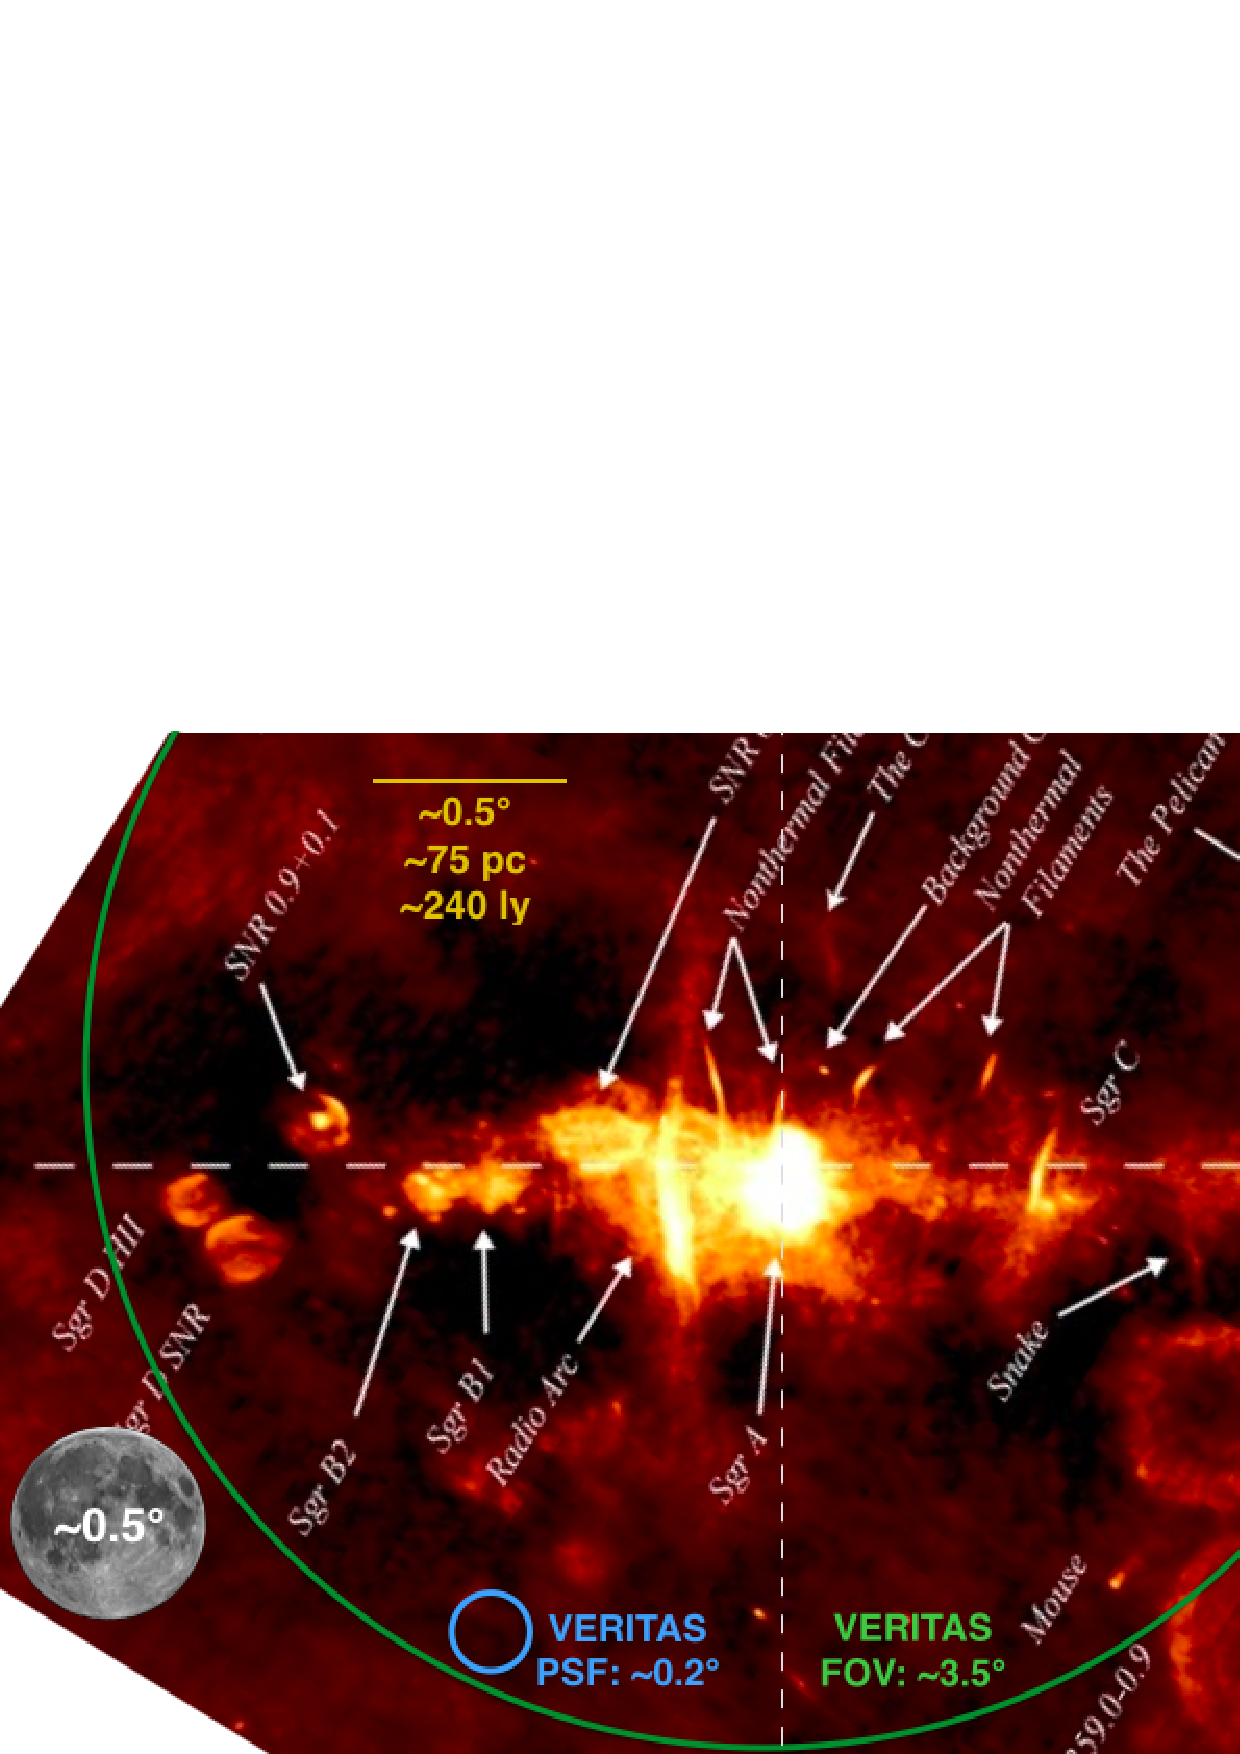
\includegraphics[width=0.95\textwidth]{images/GalacticCenterInRadio/GalacticCenterInRadio.pdf}
    \caption[Galactic Center in Radio]{
      The center of our galaxy, viewed at a radio wavelength of $\lambda=90\text{cm}$.
      The horizontal dashed line roughly represents the galactic plane, where the intersection of the dashed lines indicates the center of our galaxy.
      Supernova remnants and dust are visible in the view.
      The VERITAS field of view, the VERITAS point source spread (68\% containment), and the moon are shown for angular scale.
      Radio flux image is from Ref. \cite{galactic_center_in_radio}.}
    \label{fig_gc_radio}
  \end{figure}

  The dust, supernova remnants, and the Galactic Center itself all emit gamma rays, making detection of a dark matter halo difficult.
  The dust operates as a collision target for high-energy protons from other galaxies, whose interactions produce $\pi_0$ particles, which then decay into gamma rays.
  These dust-induced gamma rays are collectivly referred to as Diffuse Emission, and appear as a disk of gamma rays along the galactic plane.
  The supernova remnants accelerate electrons and protons outwards, which then shock into the surrounding dust and gas, producing gamma rays.
  The black hole at the Galactic Center also produces gamma rays in a point-like shape (point-like relative to the other sources), though the mechanism by which it does this is not well understood~\cite{gal_cent_still_undetermined}.

  These effects all obscure the target of this analysis, the gamma ray emission from a dark matter halo.
  This spherically-symmetric halo of gamma rays would surround the Galactic Center, decreasing in intensity the further from the center.
  The halo's spectrum would also be different from the surrounding diffuse emission.

  Once these gamma rays have been emitted, they would travel to Earth, where humans can detect them.
  This is done by using a telescope to observe the particle shower that occurs when each gamma ray hits the Earth's atmosphere.
  The VERITAS telescope has been observing gamma rays from the Galactic Center for several years.
  The data from these observations are used in this analysis.


\section{Halo Analysis}
  After several years of observation, VERITAS has accumulated \SI{108}{hours} of Galactic Center data.
  To analyze these observations, an unbinned likelihood analysis is used.
  With this analysis, the Galactic Center region is modeled with nine different dark matter halos, and the statistical existance of each halo can be calculated.
  For the spatial shape of the dark matter halo, a cuspy Einasto profile is chosen.
  For the spectral shape, only the $b\bar{b}$ annihilation channel is used.
  Each of the nine dark matter halos is modeled with a different dark matter mass $m_{\chi}$, which changes the spectrum of gamma rays produced in each $\chi\chi$ annihilation.
  
  From this analysis, no dark matter signal was found at any of these masses.
  With this null result, the next step is to calculate the upper limit on the cross-section, indicating that any $\chi$ cross-section {\color{red}(in this sentence: velocity-averaged cross-section!??)} larger than this upper limit would be visible, and can be ruled out.
  From these upper limits, new limits can be placed on the WIMP velocity-averaged cross-section at \SI{100}{TeV}.



\cleartooddpage[\thispagestyle{empty}]
\chapter{Dark Matter}

\section{Evidence for Dark Matter}

Peering out into space, there are observations on several different length scales that are attributed to dark matter.
As dark matter, by definition, does not directly interact with electromagetic light, most of the evidence for dark matter relies on a combination of gravtiational effects pulling on electromagnetic emitters, and mass distorting the spacetime paths taken by passing light.

On the smallest scales, groups of several thousand stars can be seen revolving around their center of mass, at a larger distribution of speeds than one would expect from the existing visible amount of matter.
At larger scales the optical light from galaxies, as well as hydrogen lines, can be used to measure the amount of mass and its rotational velocity around the center of galaxies.
At even larger scales, galaxy velocities can be measured and compared, x-ray telescopes can monitor the amount of hot gas, and mass-heavy areas of space will gravitationally lens background galaxies.
At the the largest scales, the measurement of oscillations in the cosmic microwave background can be used to determine the amount of dark and baryonic matter.


\subsection{$10^{19}m$ : Dwarf Galaxy Scale}
% 10^19m comes from: 
% fornax dwarf spheroidal galaxy wiki page
%    17' x 12.6' in solid angle, call it 15'
%    140kpc away  
%    140kpc * Tan(15') = 0.6kpc = 1.8*10^19m ~ 10^19m
At scales of $\nicetilde 10^{19}$m, groups of thousands stars, called satellite galaxies or dwarf galaxies, lie at the edge of the Milky Way galaxy.
Telescopes can measure the individual spectra of these stars, allowing for their velocity to be calculated.
Often, these observations focus on the Red Giant stars within these dwarf galaxies\cite{dwarf_gal_red_giant}.
By looking at the distribution of these velocities (the width of this distribution is called the velocity dispersion), the total mass of the dwarf galaxy can be inferred\cite{dwarf_gal_vel_dispersion}, \cite{dwarf_gal_vel_dispersion2}.

What makes this possible is that the velocity dispersion of a group of stars is proportional to the total mass of the graviational well.
If one starts with the virial theorem:

$2K + U = 0$

where
$K=\frac{1}{2}MV^{2}$ and $U=-\alpha \frac{GM^2}{R}$.

From a maxwell-boltzmann distribution, the dispersion of the velocities $\sigma$ is related to the original average velocity $v$ via $\sigma^2 = 3v^2$, which can be substituted into the virial theorem to give:

$blah$
??

Dwarf galaxies have mass-to-light ratios of around 5-10 $\frac{M_\odot}{L_\odot}$ (cite??).



\subsection{$10^{20}m$ : Galaxy Scale}
%
% galaxy rotation curve wiki page, M33 has curve measurements out to 50,000ly
%   50,000ly = 4.7*10^20m ~ 10^20m
At scales of $\nicetilde 10^{20}$m, the effects of Dark Matter on galaxies are observable.
In one method, the total amount of light produced by a quadrant of a galaxy is measured with telescopes.
Known mass-to-light ratios can then be used to calculate the total amount of mass within that quadrant.
This was the earliest(??) method of measuring the mass of a galaxy, producing a low value for the amount of mass.

In a second method, a galaxy's emission spectrum is observed at many positions around its disk (center, outer edges, etc).
By comparing the orientation of the disk with the doppler-shifted position of common spectral lines, one can calculate the average velocity that each chunk is travelling at around the center of the galaxy.
Newton's law of gravity can then be used to calculate the mass contained within a sphere of that same radius.
This calculation ends up with a larger amount of mass.

Mass to light ratios??

\subsection{$10^{23}m$ : Galaxy Cluster Scale}
%
% galaxy cluster wiki page
% 2-10 Mpc, call it 6Mpc = 1.85*10^23m ~ 10^23m
At scales of $\nicetilde 10^{23}$m, Dark Matter's effects on galactic clusters becomes observable by comparing three techniques.
In the first method, galaxy clusters are be massive enough to bend the images of background galaxies.
The type and amount of bending can be used to determine the mass of the intermediate galaxy.

X-Ray observations of galaxy clusters can measure the amount of hot baryonic mass.
This has been shown distinctly in the Bullet Cluster\cite{bullet}.
In this cluster, the total (baryonic+dark) mass was traced using gravitational lensing of background light.
The baryonic mass was then traced with x-rays, which are emitted by ionized gas in the region.
Figure \ref{fig:bullet} then shows these two masses overlayed.

\begin{figure}[h]
  \begin{center}
    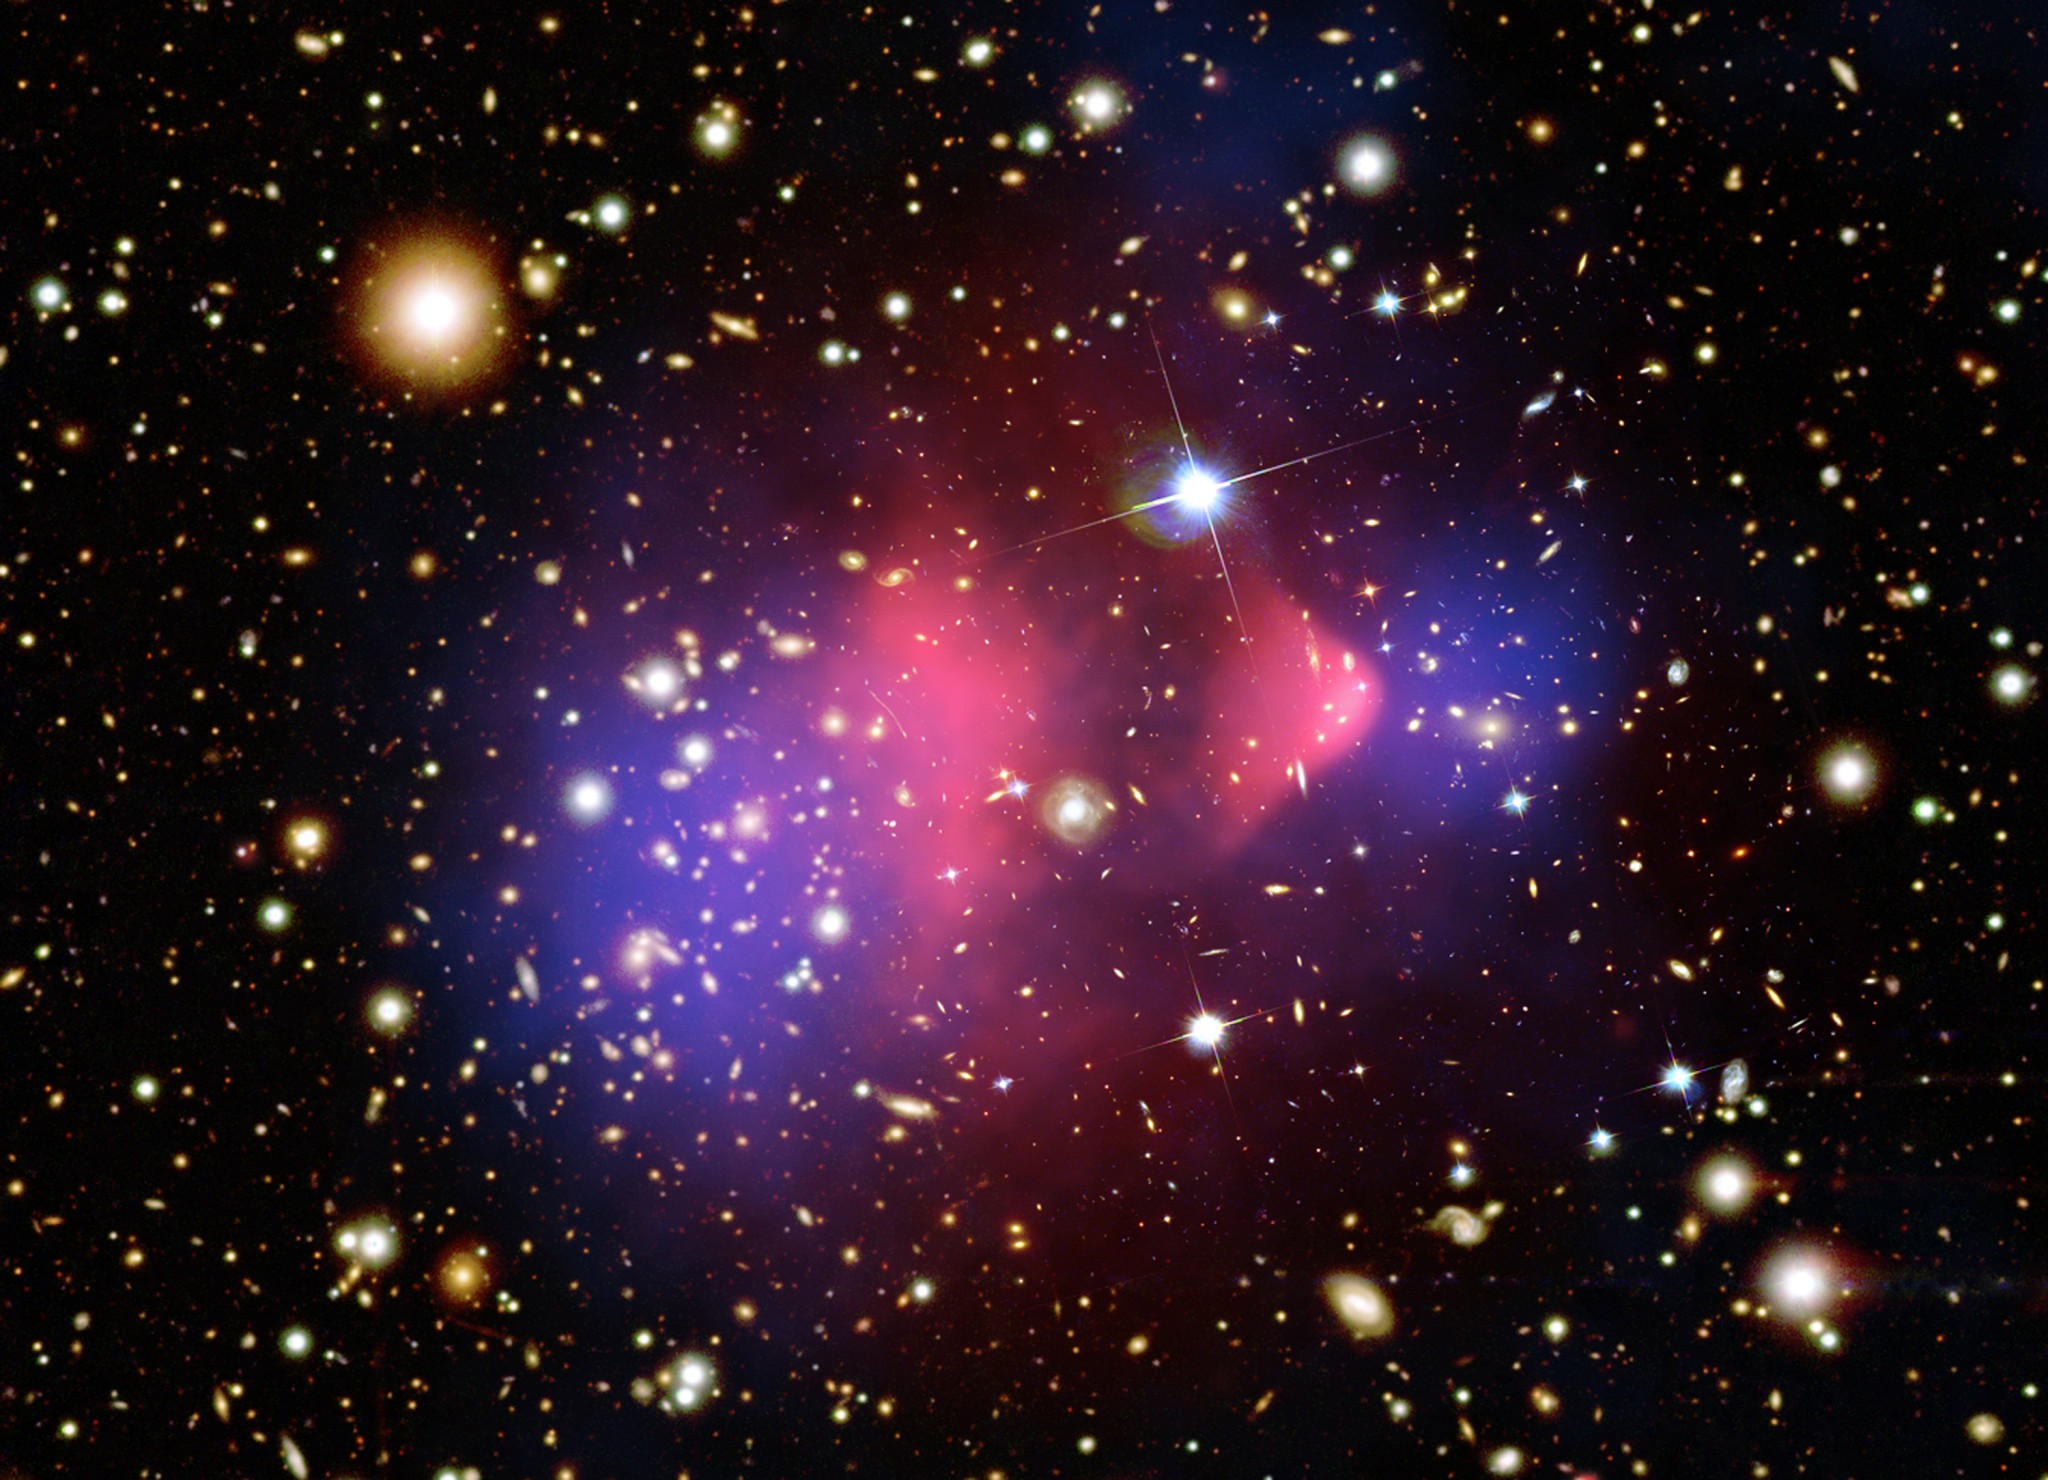
\includegraphics[width=0.95\textwidth]{images/bulletcluster.eps}
    \caption[The Bullet Cluster]{The bullet cluster\cite{bullet_cluster_combined_image}.  The blue clouds indicate the graviational lensing mass\cite{bullet_cluster}, the red represents two clouds of ionized baryons emitting x-rays\cite{bullet_cluster_chandramap}.  The remaining stars and galaxies are imaged in the optical spectrum\cite{bullet_cluster_composite}.}\label{fig:bullet}
  \end{center}
\end{figure}

Followup studies have also been done of other galaxy clusters.
Mass to light ratios??


In the second method, the velocity of different galaxies in a cluster can be measured.
By comparing the velocities of different galxies in a cluster, the contained mass within the cluster can be measured.
Mass to light ratios??

%\subsection{Inter-Cluster Scale}
% fast radio burst galaxy at z = 0.492 (http://www.nature.com/nature/journal/v530/n7591/full/nature17140.html)
% redshift to distance : d = z c / Ho (http://m.teachastronomy.com/astropedia/article/Relating-Redshift-and-Distance)
% wmap hubble constant = 70.4 (km/s)/Mpc (http://map.gsfc.nasa.gov/universe/bb_tests_exp.html)
% c = 2.99*10^8 m/s = 2.99*10^5 km/s
% 0.492 * 2.99*10^5 km/s / 70.4(km/s)/Mpc = 2089 Mpc = 6.44*10^25 m
%?? NATURE PAPER IS IN QUESTION ??
%At even larger scales of $\nicetilde 10^{25}$m, fast radio bursts and their frequency dispersion can be used to place limits on the amount of baryonic matter in the path of the burst.
%This in turn allows for upper limits to be placed on the amount of dark matter present as well.


\subsection{$10^{26}m$ : Universe Scale}
%
% age of universe (13.82*10^9 years * speed of light) = 1.307*10^26m
At the largest scale of the universe, $\nicetilde 10^{26}$m, the cosmic microwave background (CMB) has been used to measure the total amount of dark matter in the universe.
By looking at the structure of the CMB, earlier times in the universe can be studied.
Closer to the big bang, there was a point in time referred to as the 'freezout'.
Before that time, the universe was a sea of quark plasma and other particles, and the temperature was too hot to allow baryons exist for any long period of time.
After that freezout time, the temperature low enough that baryons stopped being created and annihilated.
Thus, the number of baryons that were in the universe at the freezout temperature determines how many baryons are in existance today, since there aren't any significant ways to destroy universe-scale quantities of baryons.
This freezout left an imprint of its structure, where more baryons in some places created more CMB photons, and other places had less of each.
So, by looking at this CMB structure, the total number of baryons in the universe can be measured.




\section{Dark Matter and the Standard Model}

The current paradigm of particle physics is called the Standard Model.
It describes the masses and crosssections of quarks and leptons, as well as how bosons mediate interactions between these particles.
In cosmology, the equivalent of the standard model is $\Lambda$CDM (Lambda Cold Dark Matter). 
$\Lambda$CDM describes how the universe evolved from the big bang, including the contributions of dark matter and dark energy.
It also describes how a non-relativistic (cold) dark matter particle is necessary for the current evolution of the universe.
However, either through wrong mass, wrong quantity, wrong cross section, or wrong velocity, no Standard Model particles can be cold dark matter.
This fuels suspicion than there are new, as of yet unknown particles that can fufill this role.
The two currently favored candidates are WIMPs (the subject of this thesis), and Axions.


\subsection{WIMPs}

WIMPs, or Weakly-Interacting Massive Particles, are predicted to only interact gravitationally and through weak interactions.
A major reason they are a popular dark matter candidate is due to the "WIMP Miracle".
The WIMP miracle is that the dark matter particle's predicted weak force cross section from particle physics is the same order of magnitude as predicted by cosmology.

In particle physics, a WIMP dark matter candidate would need to be around 100GeV, meaning it would have a crosssection around ?? $cm^{2}$.
In cosmology, the early expansion of the universe had an epoch where the dark matter particles froze out, where the universe was large enough that dark matter collisions became infrequent, leading to no new dark matter particles.
The time when this freezout occurred left an imprint on the Microwave Cosmic Background, which can be used to infer the cross section of the dark matter particle, which is around ?? $c^{2}$.

The fact that particle physics predicts ??$cm^{2}$, and cosmology predicts ??$cm^{2}$, is the miracle.
That two separate fields of physics end up predicting a similar dark matter cross section is highly suggestive, and is why many DM studies are devoted to the search for WIMPs.


\subsection{Axions}

Another possible dark matter candidate is the axion.
Originally theorized as a way to solve the strong CP problem ??, they also ended up being a good dark matter candidate.

Most searches for axions consist of looking for changes in photon opacity in the presence of magnetic fields.
This can occur in Earth laboratories, where a laser is shined through a strong magnetic field at an opaque wall (like several meters of concrete), then measuring the number of photons detected on the other side of the wall in a similar magnetic field.
If axions are present, the laser photons will convert into axions in the presence of the magnetic field, pass through the wall, and convert back into photons again on the other side.

In astrophysical scales, this can be done by examining distant galaxies.
Due to the haze of particles in between galaxies, most photons from distant galaxies is lost due to interactions.
If axions are present, extremely distant galaxies that are normally too dim may become detectable.


\subsubsection{Other Potential Candidates}

Other potential ideas that could explain Dark Matter's effects are Massive Compact Halo Objects, or MACHOs.
While WIMPs and Axions are particle-scale dark matter candidates, MACHOs are instead stellar-scale candidates.
These could be either large planets that weren't quite big enough to start fusing hydrogen, or primordial black holes.
Primordial black holes are predicted to have been created shortly after the big bang.
As there is presently no known mechanism for reducing their numbers, the majority of these black holes would be capable of surviving to the present time.

In either case, as these halo objects would be neither strongly absorptive or emissive at any electromagnetic frequency, they would be difficult to detect.
Most theories invovlving MACHOs are constrained by measurements of the universe's total baryonic mass from the measurements of the CMB.
Star-Star gravitational lensing can in principle be used to detect these compact objects, but this technique is difficult and has large systematic errors (macho survey citation??).
While there are significant constraints\cite{pbh_highly_constrained}, primordial black hole mergers can in principle be detected with graviational wave detectors like LIGO\cite{dm_with_ligo}, though at present more observation time is needed.



\section{Dark Matter Search Techniques}


There are three categories of searches for dark matter particles.
Direct Detection experiments attempt to discern when a dark matter particle directly strikes a volume of detection mass, stored deep underground.
Indirect Detection experiments attempt to look for secondary products of dark matter interactions, usually through astrophysical searchs.
Collider searches attempt to produce a dark matter particle through controlled collisions of standard model particles.

% direct
Direct searches consist of an interaction mass, surrounded by light, heat, and acoustic sensors, usually buried deep underground.
These sensors attempt to detect a signal from when a particle strikes the enclosed interaction mass, and discern how much mass and energy the incident particle had.
Most of these detectors are either solid blocks of ??, or liquified gasses like Xenon.

% collider
Collider searches involve accelerating particles in particle accelerators, smashing them together, and searching the resulting explosion of particles for evidence of dark matter particles.

% indirect
Indirect searches involve observing regions of space with telescopes, either looking for secondary particles that may have been produced by a dark matter collisions, or for gravitational effects, like lensing.
The analysis described later in this thesis is an indirect search, examining whether gamma rays near the galactic center match the given predicted shape of a dark matter halo.
Much of the evidence for dark matter, as detailed in section ??, comes from indirect searches.



\section{Mass and Cross-section}


\section{Halo Structure}
Numerical simulations have been performed to simulate the structure of dark matter halos.
On galactic scales, these halos can be modeled with several different density profiles.
Three of the primary profiles are the Burkert, the Einasto, and the Zhao profile.
Each profile describes the mass/volume density of dark matter at a distance r from the halo center.

A Burkert profile (\cite{burkertprofile}) has the form

$ \rho_{DM} \left( r \right) = \frac{ \rho_o r_o3}{ \left( r + r_o \right) \left( r^2 + r_o^2 \right)} $ \label{eqn:burkert}

where $r_o$ is the scale radius of the halo, and $\rho_o$ is the scale density, the density at the scale radius.

The Einasto profile (\cite{einastoprofile1},\cite{einastoprofile2}) has the form

$ \rho_{DM} \left( r \right) = Exp \left( - \frac{2}{\alpha} \left( {\left( \frac{r}{r_o} \right)}^{\alpha} - 1 \right) \right)$ \label{eqn:einasto}

The Zhao profile (\cite{zhaoprofile}) has the form

$ \rho_{DM} \left( r \right) = \frac{\rho_o}{ {\left( \frac{r}{r_o} \right)}^{\gamma} {\left( 1 + {\left( \frac{r}{r_o} \right)}^{\alpha} \right)}^{ \left(\beta - \gamma \right) / \alpha} } $ \label{eqn:zhao}

where $\gamma$ is the slope of the density profile when $r << r_o$, $\beta$ is the slope when $r >> r_o$, and $\alpha$ determines how large the transition region is between $\gamma$ and $\beta$.
A larger $\alpha$ means a smaller transition region.

These profiles can then be used to calculate the spatial distribution of gamma-rays.
For annihilating dark matter, $\rho\left(r\right)^2$ must be integrated along the line of sight.

$ \frac{d\Phi}{dE d\Omega}= \frac{ \left \langle \sigma v \right \rangle }{8 \pi m_\chi^2} \frac{dN}{dE} \int \rho^2 dl $ \label{eqn:dmflux}

?? equation also depends on if particle is symmetric? 8 $\pi$ may change or something ??




\cleartooddpage[\thispagestyle{empty}]

\newcommand{\Lim}[1]{\raisebox{0.5ex}{\scalebox{0.8}{$\displaystyle \lim_{#1}\;$}}}
\renewcommand{\labelitemi}{\textbullet}
\newcommand{\pip}[1]{$\pi^{+}$}
\newcommand{\pim}[1]{$\pi^{-}$}
\newcommand{\pio}[1]{$\pi^{0}$}
\newcommand{\sv}{\left < \sigma v \right >}

\chapter{Gamma Rays and Dark Matter}\label{ch_gamma}


This analysis searches for dark matter using gamma rays, thus a discussion of gamma rays and their properties is necessary.
In this chapter three different topics are discussed, including background gamma rays, dark matter gamma rays, and detecting gamma rays in general..
The first is the astrophysical mechanisms that produce gamma rays, a background for detecting dark matter gamma rays..
The second is how dark matter around the Galactic Center can produce gamma rays.
The third topic is how gamma rays induce air showers in the Earth's atmosphere.

\section{Production of TeV Gamma Rays}

  There are several mechanisms that can produce photons with TeV energies.
  A gamma ray can start as a low-energy photon, then gain significant energy from electroweak interactions with electrons, referred to as a leptonic production.
  Alternately, a gamma ray can be created from a high-energy proton colliding with another proton, which produces $\pi^0$'s that decay into gamma rays, referred to as hadronic production.
  However, leptonic and hadronic production are separate from how gamma rays are produced by dark matter.
  Instead, two WIMP dark matter paritlces may annihilate (directly or indirectly) into gamma rays, as is discussed in Section~\ref{dm_spectral}.

  In leptonic production, electrons and low-energy photons collide, transferring energy to the photon.
  This interaction is called upscattering or inverse Compton scattering~\cite{compton_effect}, and its feynman diagram is shown in Figure~\ref{fig:inv_compt_feyn}.
  
  \begin{figure}[ht]
    \centering
    \includegraphics[width=0.45\textwidth]{images/feynman_particles/inversecompton.pdf}
    \caption[Inverse Compton Scattering Feynman Diagram]{
      Feynman diagram of inverse Compton scattering, where an electron upscatters a low-energy photon (red) to produce a higher-energy (blue) photon.
    }
    \label{fig:inv_compt_feyn}
  \end{figure}
  \FloatBarrier
  
  In inverse Compton scattering, a field of photons with an electron present will gain energy according to Equation~\ref{eqn:inv_compt_en_gain_rate}~\cite{inv_compt1,inv_compt2},
  
  % https://eud.gsfc.nasa.gov/Volker.Beckmann/school/download/Longair_Radiation3.pdf equation 11
  \begin{equation}\label{eqn:inv_compt_en_gain_rate}
    \frac{dE}{dt} = \frac{4}{3} \: \sigma_{t} \: U \: c \: \gamma^2 \: \frac{ v^2 }{ c^2 } \;\; ,
  \end{equation}

  where
  
  \begin{itemize}
    \item $\sigma_{t}$ is the Thomson cross section, $\frac{8\pi}{3} \left ( \frac{\alpha \hbar c}{m c^2} \right )$
    % Thomson cross section is from wikipedia.org/wiki/Thomson_scattering
    \item $c$ is the speed of light in vaccum,
    \item $\gamma$ is the Lorentz factor,
    \item $U$ is the energy density of the photon field in the rest frame of the electron (e.g. $Uc=N\hbar \omega c$), and 
    \item $v$ is the velocity of the electron in the laboratory frame.
  \end{itemize}

  The average energy $E_{up}$ of photons upscattered this way can be calculated via
  
  % https://eud.gsfc.nasa.gov/Volker.Beckmann/school/download/Longair_Radiation3.pdf equation 15
  \begin{equation}\label{eqn:inv_compt_avg_up_en}
    E_{up} = \frac{4}{3} \: \gamma^2 \: E_{0} \;\;.
  \end{equation}
  
  % me = 5e5 eV (mass of electron)
  
  % formula for calculating gamma (lorentz factor) from relativistic kinetic energy
  % Ek = mc^2 / sqrt(1-v^2/c^2) - mc^2
  % Ek + mc^2 = mc^2 / sqrt(1-v^2/c^2)
  % ( Ek + mc^2 ) / mc^2 = 1 / sqrt(1-(v^2/c^2)) = g
  
  % lorentz factor for various kinetic energy electrons
  % Ek = 5e5  eV, 500 KeV, g =   2
  % Ek = 1e6  eV,   1 MeV, g =   3
  % Ek = 1e7  eV,  10 MeV, g =  21
  % Ek = 1e8  eV, 100 MeV, g = 201
  % Ek = 1e9  eV,   1 GeV, g = 2e3
  % Ek = 1e10 eV,  10 GeV, g = 2e4
  % Ek = 5e11 eV, 500 GeV, g = 1e6
  
  % calculating the energy in eV of a green photon
  % lg = 550e-9 m  = 5.5e-7 m
  % c = l*w
  % wg = c / lg
  % wg = 2.99e8 m/s / 5.5e-7 m = 5.4e14 1/s
  % E  = hbar w
  % hbar = 1.05e-34 m^2 kg / s (reduced planck constant)
  % 1 J = 6.24e18 eV
  % Eg = hbar wg
  % Eg = 1.05e-34 m^2 kg / s    * 5.4e14 1/s * 6.24e18 eV/J
  % Eg = 1.05 * 5.4 * 6.24 e-34 e14 e18 eV
  % Eg = 35.3e-2 eV
  % Eg = 0.35 eV (energy of a green photon)
  
  % 500 GeV electron upscatters a 0.35 eV photon (green) into a ? eV photon?
  % gamma = (Ek + Ee) / Ee
  % gamma = ( 5e11 eV + 5e5 eV ) / 5e5 eV
  % gamma = 1e6
  % Eup = (4/3) * gamma^2 * Eg
  % Eup = (4/3) * 1e12 * 0.35 eV
  % Eup = 4.67e11 eV = 467 GeV
  
  The parameter $E_{0}$ is the energy of the original photon.
  At Earth, astrophysical electrons are detected at energies of \SI{500}{GeV}~\cite{500GeVElectrons,fermi_electron}.
  At these energies, the Lorentz factor is $\gamma = 10^6$.
  With this Lorentz factor, upscattered photons can increase their energy by up to\footnote{This is the maximum average energy gain when the upscattered photon is emitted back along its original trajectory.} $\gamma^{2} = 10^{12}$.
  For example, a green photon ($\lambda_{\textrm{green}}=550\,\textrm{nm}$, $E_{\textrm{green}}=0.3\,\textrm{eV}$) could be upscattered to as high as \SI{467}{GeV}, becoming a gamma ray detectable by VERITAS.
  
  In order to efficiently produce gamma rays via this method, a population of high-energy electrons is needed.
  One environment for producing these electrons is around pulsar wind nebulae.
  Because pulsars spin rapidly, they produce strong magnetic fields.
  For example, the pulsar at the heart of the Crab nebula has a surface magnetic field strength of \SI{e12}{G}~\cite{pwn_evolution}, much larger than Earth's $\sim$\SI{0.5}{G}~\cite{earth_geomag}.
  These strong magnetic fields provide an environment for producing and accelerating charged particles.
  In these strong magnetic fields, ambient photons can convert into $e^{+}e^{-}$~\cite{pwn_pairprod2,pwn_pairprod3}.
  The probability $\Upsilon$ (0-1) of a photon pair-converting in a magnetic field is calculated by via 
  
  \begin{equation}\label{eqn:pwn_pairprod}
    \Upsilon = \frac{E}{mc^2} \frac{H}{c} \frac{e \hbar}{m^2c^2} \;\;,
  \end{equation}
  
  where $E$ is the photon energy, $H$ is the ambient magnetic field strength, $e$ is the electron charge, and $m$ is the mass of the electron~\cite{pwn_pairprod3}.
  The factor $\frac{e \hbar}{m^2c^2}$ acts as a threshold magnetic field strength, above which the conversion rate becomes significant.
  For electrons the threshold is $\frac{1}{4.4\times10^{13}\,\textrm{Gauss}}$, similar in scale to the pulsar's surface magnetic field strength.
  %
  % paper : https://journals.aps.org/rmp/pdf/10.1103/RevModPhys.38.626
  % High-Energy Electromagnetic Conversion Processes in Intesnse Magnetic Fields, T. Erber, 1966
  %    NOTICE: This paper has a mistake in equations 1.1 and 1.1a (a 'c' in 1.1a should be moved to 1.1, thats all)
  %
  % e = 1.602e-19 C
  % hbar = 1.05e-34 J*s
  % m_electron = 9.11e-31 kg
  % c = 2.98e8 m/s
  % 1 Gauss = 1e-4 kg/ A*s^2 = 1e-4 kg C^-1 s^-1
  % 
  % factor = e hbar / m^2 c^2
  %        = 1.602e-19 C * 1.05e-34 J*s / (9.11e-31 kg)^2 (2.98e8 m/s)^2
  %        = 4.4e13 G
  
  Charged particles can also be accelerated by a pulsar's magnetic fields, in a process called magnetic reconnection, shown in Figure~\ref{fig:magcon}.
  In this mechanism, two oppositely oriented magnetic fields move towards each other (Figure~\ref{fig:magcon}.a), due to the field lines being frozen into the local plasma.
  As the magnetic field lines merge (Figures \ref{fig:magcon}.b and c), induced current flows produce electric fields (Figure~\ref{fig:magcon}.d) that {\color{red}can accelerate (what is the mechanism called?? -maria)} charged particles~\cite{magcon_crab,magcon_schopper,magcon_review,gamma_pwn1,gamma_pwn2,magconsim2011,magconsim2014,magcon_particleaccel}.
  
  \begin{figure}[ht]
    \centering
    \begin{tabular}{m{1cm}m{10cm}}
      (a) & \includegraphics[width=0.6\textwidth]{images/magnetic_reconnection/diagram_1_cr.pdf} \\
      (b) & \includegraphics[width=0.6\textwidth]{images/magnetic_reconnection/diagram_2_cr.pdf} \\
      (c) & \includegraphics[width=0.6\textwidth]{images/magnetic_reconnection/diagram_3_cr.pdf} \\
      (d) & 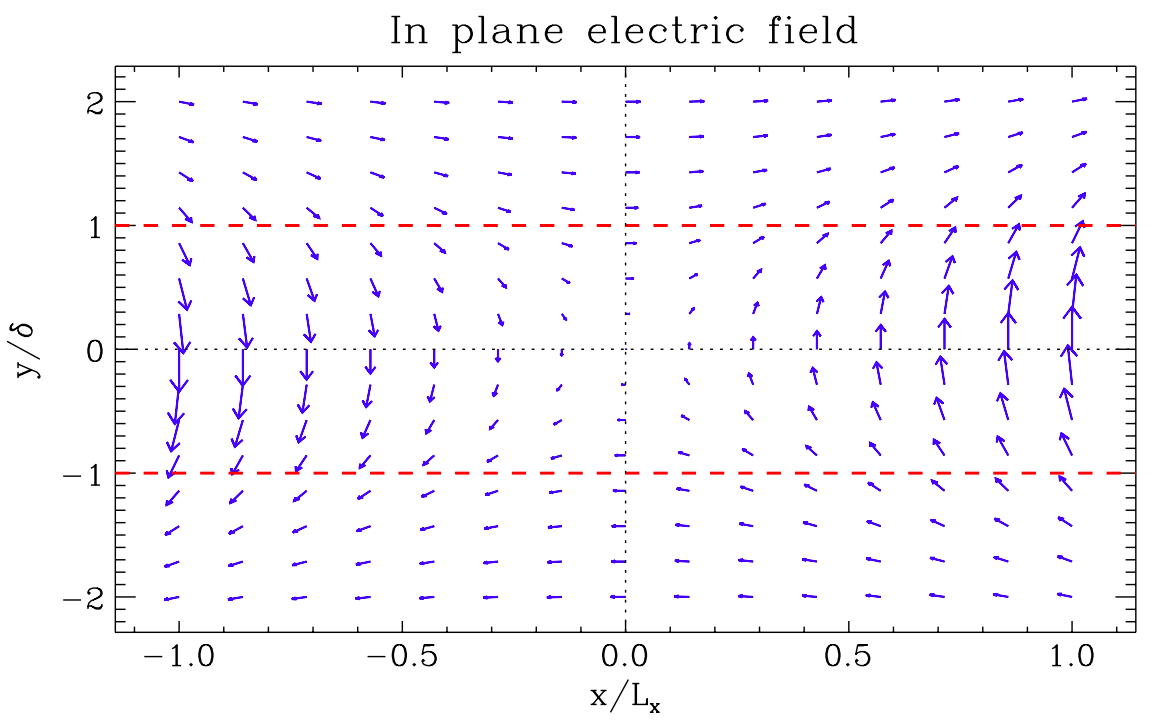
\includegraphics[width=0.6\textwidth]{images/magnetic_reconnection/magcon_efieldlines.pdf}
    \end{tabular}
    \caption[Magnetic Reconnection]{
      Reconnection of two magnetic fields.
      In (a), two oppositely-pointing magnetic fields move into each other.
      In (b), reconnection starts to occur.
      In (c), reconnection occurs, and plasma moves outwards along the $y=0$ axis.
      In (d), the resulting electric fields from the moving plasma are shown in this scenario, from Ref.~\cite{magcon_crab}.
      In these figures, $\delta$ and $\textrm{L}_{\textrm{x}}$ are the distance parameters of the reconnection area.
    }
    \label{fig:magcon}
  \end{figure}
  
  
  \FloatBarrier
  % Use figure 2 in http://iopscience.iop.org/article/10.1088/0004-637X/746/2/148/pdf
  
  % Use these sources, to get an idea of the electric field strengths doing the accelerating
  % http://iopscience.iop.org/article/10.1088/0004-637X/746/2/148/pdf
  % https://aip.scitation.org/doi/pdf/10.1063/1.873696
  % https://www.annualreviews.org/doi/pdf/10.1146/annurev-astro-082708-101726
  % something is still missing, can't find complete description of E field
  
  
  
  %The electric field in Figure~\ref{fig:magcon}.d is able to accelerate charged particles, and can be calculated with Equation~\ref{eqn:magcon_efield},
  %\begin{equation}\label{eqn:magcon_efield}
  %  \hat{E} = -\hat{V} \times \frac{B_{z}}{c} \;\; .
  %\end{equation}
  %In Equation~\ref{eqn:magcon_efield}, 
  %\begin{equation}
  %  \hat{V} = \left ( c \frac{x}{L_x} \cosh^{-2} \left ( \frac{y}{\delta} \right ),-c\beta \tanh \left ( \frac{y}{\delta} \right ), 0 \right )
  %\end{equation}
  %From \cite{magcon_crab}, equations (2) and (3).
  % 
  %\begin{equation}
  %  \hat{B} = \left ( B_0 \tanh \left ( \frac{y}{\delta} \right ), \beta B_0 \frac{x}{L_x}, 0 \right )
  %\end{equation}
  %From \cite{magcon_crab}, equations (1) and (4).
  % 
  %But this results in:
  %\begin{equation}
  %  \hat{E} = \left (  0, 0, B_0 \frac{x^2}{L_x} \beta \sech \frac{y}{\delta}^2 - B_0 \beta \tanh \frac{y}{\delta}^2 \right )
  %\end{equation}
  %Which doesn't match the plot in Figure~\ref{fig:magcon}.d .

  Another mechanism that produces high-energy charged particles is Fermi acceleration~\cite{fermi1949,highenergyelectron_snr}.
  In general, this acceleration imparts energy to charged particles when they are reflected by an oncoming magnetic field.
  
  One environment where this can happen often is in the shockfront of a supernova, where the mechanism is called diffusive shock acceleration~\cite{dsa1,dsa2,dsa3,dsa4,dsa5}.
  During and after a supernova's initial {\color{red}detonation (another word??)}, charged fermions are quickly heated.
  These heated particles then expand outwards, creating a moving shockfront at the boundary between the expanding particles and the surrounding Inter-Stellar Medium (ISM).
  These expanding particles {\color{red}bring their own magnetic fields (how do they bring their own magnetic fields??)}, which reflect charged particles.
  As the shockfront expands, it also runs into the ambient magnetic fields in the ISM, which can also reflect charged particles.
  This shockfront is shown in Figure~\ref{fig:snr_shockfront}.

  \begin{figure}[ht]
    \centering
    \includegraphics[width=0.75\textwidth]{images/snr_shockfront/shockfront_diagram.pdf}
    \caption[Supernova Shockfront]{
      Diagram of supernova shockfront.
      Relative to some inertial observer, the supernova plasma expands at velocity $v_s$, while the ISM moves at velocity $v_m$.
    }
    \label{fig:snr_shockfront}
  \end{figure}
  
  At the shockfront, particles that cross it are reflected off the magnetic fields on the other side, gaining a small amount of energy each time.
  Over many crossings, charged particles can gain high energies, though the higher the energy of the particle, the more likely it can escape the shockfront, since it's gyroradius increases as its energy increases.
  The amount of energy gained is governed by a parameter $\beta$, in Equation~\ref{eqn:snr_beta}, 
  
  \begin{equation}\label{eqn:snr_beta}
    \beta = 1 + \frac{v_s}{c} \;\; .
  \end{equation}
  
  This $\beta$ parameter can be interpreted as the fractional energy gain per crossing, as in Equation~\ref{eqn:snr_beta_en},

  \begin{equation}\label{eqn:snr_beta_en}
    E_{i+1} = \beta E_{i} \;\; .
  \end{equation}
  
  The $E_i$ parameter is the average energy of a charged particle after it's $i^{\textrm{th}}$ crossing.
  The energy gain $\beta$ factor influences the energy spectrum of the escaping charged particles, but so too does $P$, the probability that the charged particle remains trapped at the shockfront after each crossing.
  This probability $P$ can be calculated with
  
  \begin{equation}\label{eqn:snr_prob}
    P = 1 - \frac{v_s}{c}
  \end{equation}
  
  With this probability $P$ and the energy gain $\beta$, the energy spectrum of particles that permanently escape the shockfront can be calculated by
  
  \begin{equation}\label{eqn:snr_spec}
    \frac{dN}{dE} \approx E^{ \frac{\log P}{\log \beta} - 1 }
  \end{equation}
  
  With Equations~\ref{eqn:snr_prob} and \ref{eqn:snr_beta}, the spectrum from Equation~\ref{eqn:snr_spec} can be simplified.

  \begin{equation}\label{eqn:snr_simplify}
    \begin{split}
       \log P     & = \log \left ( 1 - \frac{v_s}{c} \right ) \approx - \frac{v_s}{c} \\
       \log \beta & = \log \left ( 1 + \frac{v_s}{c} \right ) \approx + \frac{v_s}{c} \\
    \end{split}
  \end{equation}
  
  Equation~\ref{eqn:snr_spec} then simplifies to
  
  \begin{equation}\label{eqn:snr_spec_final}
    \begin{split}
      \frac{dN}{dE} & \approx E^{ \frac{\log P}{\log \beta} - 1 } \\
                    & \approx E^{ \frac{ -\frac{v_s}{c} }{ +\frac{v_s}{c} } - 1 } \\
                    & \approx E^{ -1 - 1 } \\
      \frac{dN}{dE} & \approx E^{ -2 } \;\; .
    \end{split}
  \end{equation}

  In Equation~\ref{eqn:snr_spec_final}, the exponent is often referred to as the spectral index $\gamma$.
  From this diffusive shock acceleration, the spectral index of charged particles is approximately -2.
  This is quite close to the observed extragalactic cosmic ray spectral index range of \SIRange{2.0}{2.2}, but additional effects (discussed in Ref.~\cite{cosmicrayspectrumorigin}) may soften this index to get to the observed galactic cosmic ray spectral index of $\approx{}3.7$ {\color{red}(orel highlighted 2.0-2.2 and 3.7??)}.
  The spectral index's dependence on $P$ and $\beta$ is shown in two plots in Figure~\ref{fig:snr_spectrum}.
  The top plot in Figure~\ref{fig:snr_spectrum} shows how changing $\beta$, the energy gain per shockfront crossing cycle, and the bottom plot shows the differential spectra with the spectral indicies from the top plot.
  From these two plots, it can be seen that increasing the energy gain per crossing cycle $\beta$ creates a harder spectrum of particles with more higher energy particles, since they can reach escape energies in fewer cycles.
  It can also be seen that trapping more particles at the shockfront (higher $P$) also creates a harder spectrum of escaping particles, as particles can be contained for more cycles, gaining more energy before escaping~\cite{dsa6}.

  \begin{figure}[ht]
    \centering
    \includegraphics[width=0.8\textwidth]{images/snr_shockfront/snr_spectrum.pdf}
    \caption[Supernova Diffuse Acceleration Spectral Indicies]{
      The top plot shows the spectral indicies produced by various combinations of $\beta$, the fractional energy gained by a particle in one crossing cycle (upstream $\rightarrow$ downstream $\rightarrow$ upstream), and $P$, the average chance a particle is unable to escape the shockfront.
      The contours for three spectral indicies $\gamma$ are shown.
      For example, at the orange triangle, each crossing cycle increases a particles energy by a factor of 1.10, while it has a 90\% chance of being permanently trapped, which produces particles with a spectral index of $\gamma=-2.1$.
      The bottom plot shows the differential flux produced by power laws with the three spectral indicies shown in the top plot.
    }\label{fig:snr_spectrum}
  \end{figure}
  
  \FloatBarrier
  
  % slides on supernova shockwaves
  % https://isapp2012paris.sciencesconf.org/conference/isapp2012paris/Stefano_Gabici_three.pdf
  
  % Drury, 2012, "Origin of Cosmic Rays"
  % https://doi.org/10.1016/j.astropartphys.2012.02.006
  % Diffusive shock acceleration, 
  
  % https://www.annualreviews.org/doi/pdf/10.1146/annurev.aa.22.090184.002233 , pg 435:
  %   2 shockfronts, travelling at v1 and v2= v1 * 3/4
  %   v1 = B1 * c # velocity of the collisionless shockfront (just the B fields)
  %   v2 = B2 * c # velocity of the gas particles
  %   1 crossing cycle = reflect off each shock once = E * B2 * 4/3 increase in particle energy
  %   particle tends to escape after (B1-B2)*1/4 crossing cycles


  Protons accelerated in this manner form the majority of the showers detected by the VERITAS telescope, forming an irreducible background in the Galactic Center observations.
  This background is irreducible due to the fact that the Cherenkov images of proton and gamma-ray air showers have many similarities, and cannot be identified with perfect accuracy.
  
  Both of these processes, magnetic reconnection and diffusive shock acceleration, can accelerate protons, electrons, or any other charged particles.
  When these processes produce electrons with high energies, these electrons can then upscatter ambient photons to TeV energies.
  Additionally, electrons spiralling through magnetic fields can produce synchrotron photons at X-ray energies, meaning fewer upscatters are needed to reach TeV energies~\cite{self_compton}.

  In hadronic processes, protons can be accelerated ($p_{accel}$) by Fermi acceleraton, by a supernova remnant~\cite{proton_snr_accel}, or as part of an active galactic nucleus jet~\cite{hadronic1,hadronic2}.
  {\color{red}(Maybe add just one sentence saying that protons can be accelerated in the same way as the electrons you discussed before, just to give it a bit more importance?? -orel)}
  Then, upon striking an ambient proton ($p_{ambient}$), the interaction can, in some cases, produce $\pi^{+}\pi^{+}\pi^{0}$, and other particles $X$~\cite{pp_pion,pp_pion2,pp_pion3}.
  
  \begin{equation}\nonumber
    p_{accel} + p_{ambient} \rightarrow \pi^+ + \pi^+ + \pi^0 + X
  \end{equation}

  While other products from the $pp$ interaction may also produce gamma rays, the $\pi^0$ decay is the dominant production channel.
  The $\pi^{0}$ then quickly (\SI{8.5e-17}{s}~\cite{pdg2016}) decays into two gamma rays.
  Because each pion resulting from the original $pp$ interaction tends to receive $\frac{1}{3}$ of the original proton's kinetic energy {\color{red}(what fraction does the X receive?? -maria)}, and the $\pi^0$ decays into two gamma rays, each gamma ray ends up with \nicetilde$15\%$ of the original proton's kinetic energy.
  %In the rest frame, the $\pi^0$ has a mass of \SI{135}{\MeV}~\cite{pdg2016}, so each photon ends up with \SI{67.5}{\MeV}.
  %This means that in the rest frame,
  For example, a proton with \SI{10}{TeV} of kinetic energy will eventually produce two \SI{1.5}{TeV} gamma rays.
  
  Much of the diffuse gamma-ray component of the galactic disk is due to extra-galactic high-energy protons colliding with the protons of the galactic plane~\cite{GalacticDiffuseGammaRays,extragalactic_agn}.
  Active galactic nuclei posess particle jets, which can accelerate particles when the jet shocks into the extragalactic medium.

  \subsection{Dark Matter Interactions}\label{dmgammaproduction}
    
    The general dark matter particle searched for in this thesis is a WIMP.
    This WIMP may be detectable by three general search schemes, illustrated in Figure~\ref{fig:3_searches}.

    % add popular figure for the three detection type
    \begin{figure}[ht]
      \centering
      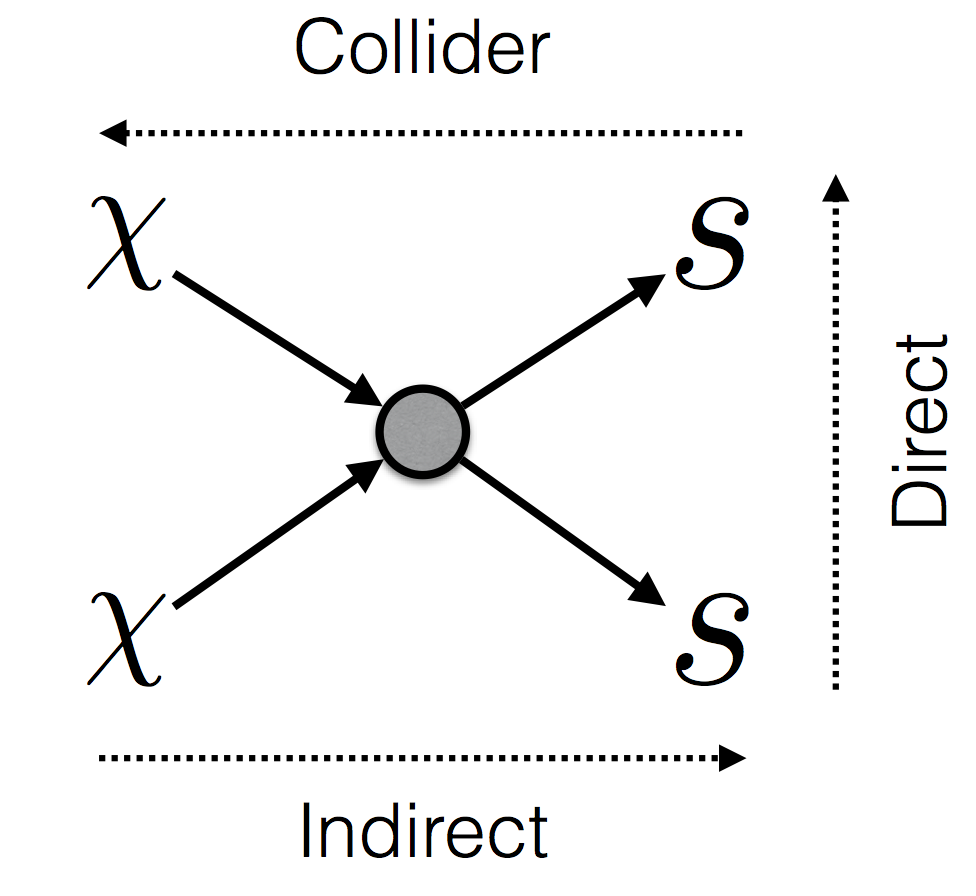
\includegraphics[width=0.65\textwidth]{images/3waystodetect/3waystodetect.pdf}
      \caption[Three Search Techniques]{
        The three general search techniques for dark matter.
        The $\chi$ is a dark matter particle, while $s$ is a standard model particle.
      }
      \label{fig:3_searches}
    \end{figure}
    
    In collider searches, $ss \rightarrow \chi\chi$, standard model particles ($ss$) are accelerated into collisions with each other within a detector, and the resulting particle fragments are measured by a slew of detectors~\cite{atlas,cms}.
    These detectors include scintillation crystals with avalanche photodiodes and silicon strip detectors.
    Some of these detectors are within magnetic fields that curve charged particles, aiding in their measurement.
    Since the initial particles are accelerated to known energies, and the output fragment particles are well measured, searching for any break from conservation laws may hint at dark matter particles. 
    
    For direct searches, $\chi s \rightarrow \chi s$, sensitive particle detectors are built deep underground.
    When a WIMP scatters off of a nucleus within the detector, the nuclear recoil can be observed, through signals such as crystal phonons, excitation and release of photons, or ionization.
    Being underground shields the detectors from cosmic rays, which create background collisions that can mimic WIMP signals.
    In liquid Xenon detectors, particle collisions in the liquid produce UV photons and electrons, which are used to infer the presence of WIMPS~\cite{direct_lux,direct_xenon}.
    Cryogenic detectors use pucks of germanium and silicon to measure particle collisions.
    These collisions produce detectable ionization and phonon signals, which are used to classify the incident particle~\cite{direct_cdms}.
    Scintillation detectors are built with crystals like titanium-doped sodium iodine.
    When an external particle collides with one of the nuclei within the crystal, that nucleus becomes excited, and then relaxes by releasing a photon~\cite{direct_dama}.
    However, to date no substantial dark matter signal has been detected with these methods~\cite{direct_dm_detection}.
    
    For indirect searches, $\chi\chi \rightarrow ss$, dark matter particles may annihilate or decay into standard model particles.
    Observatories then search for excesses of these particles, excesses that cannot be explained by known astrophysics.
    This analysis searches for an excess of gamma rays, as the center of our galaxy is believed to host a dark matter halo.
    This spherical halo would allow for many $\chi\chi$ annihilations, producing gamma rays via: 
    
    $$\chi\bar{\chi} \rightarrow S\bar{S} \rightarrow \gamma\gamma$$

    where $S\bar{S}$ can be any quark or lepton particle-antiparticle pair ($t\bar{t}$, $u\bar{u}$, $c\bar{c}$, $s\bar{s}$, $e^{-}e^{+}$, etc).
    These different annhilation channels can produce different spectra of gamma rays, which will also vary based on the WIMP mass and cross section chosen.
    This is described further in Section \ref{dm_spectral}.

\FloatBarrier

\section{Galactic Center}
  
  The Galactic Center is a complex region of space, with many astrophysical sources of gamma rays.
  At its heart is a supermassive black hole around which gamma-ray emission is observed, though the production mechanism is still under debate.
  There are other gamma-ray sources as well, including dust along the galactic plane, supernova remnants, and inverse compton emission {\color{red}(is there a graphic that illustrates the diversity?? -maria)}.
  {\color{red}(inverse compton emission is not the same 'class' as dust and supernova remnants.  I would change or remove.  See also comment below about this, maybe change both to the same thing?? -orel)}
  The TeV gamma-ray emission from a few of these sources is visible in Figure~\ref{fig:hess_plane}.
  
  \begin{figure}[ht]
    \centering
    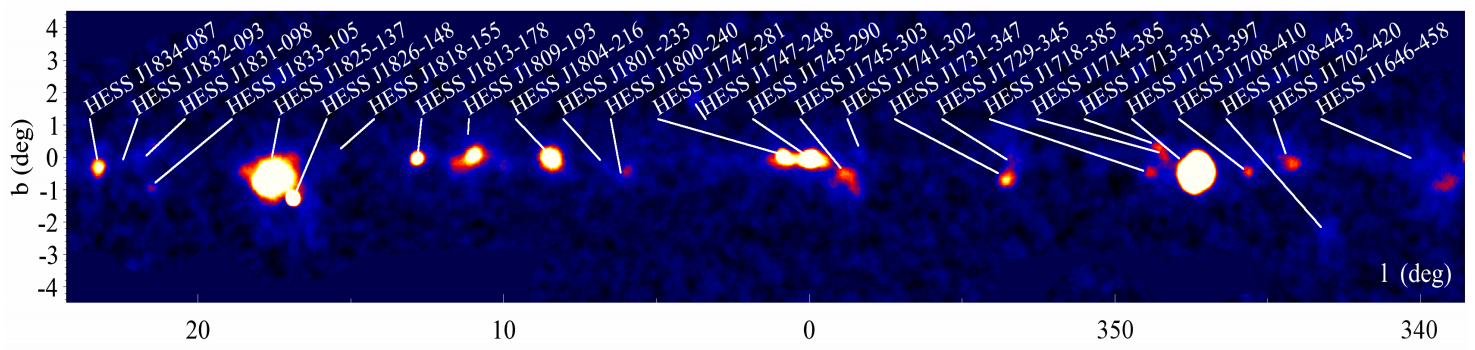
\includegraphics[width=0.98\textwidth]{images/hess_plane_survey/survey.pdf}
    \caption[HESS GC Survey]{
      Signifiance map of the Galactic Center, from the HESS Galactic Plane Survey~\cite{hess_gc_plane}.
      \CaptionBlankLine
    }
    \label{fig:hess_plane}
  \end{figure}
  
  One of the prominent gamma-ray emitters near the Galactic Center~\cite{gc_pointsrc_hess,gc_pointsource_hess2,gc_veritas_pointsource,gc_magic_pointsource} happens to have several stars orbiting it.
  Through kinematic observations of these nearby stars, it has been inferred that a supermassive black hole is present there, with a mass of \SI{4e6}{ \Msol{} }~\cite{sgra_massdist}.
  The VERITAS signifiance skymap of this Galactic Center region is shown in Figure~\ref{fig:veritas_gc_ridge}.
  
  \begin{figure}[ht]
    \centering
    \includegraphics[width=0.95\textwidth]{images/veritas_gc_ridge/ridge.pdf}
    \caption[VERITAS View of the Galactic Center Ridge]{
      Galactic Center Ridge, from Ref.~\cite{VeritasGCRidge2015}.
      \CaptionBlankLine
    }
    \label{fig:veritas_gc_ridge}
  \end{figure}

  The mechanism that produces these TeV gamma rays is still under debate.
  While a dark matter interpretation is intriguing~\cite{gc_pnt_is_dm1,gc_pnt_is_dm2}, there are several non-dark-matter models that might explain the observed features.
  {\color{red}One model that explains possibility (orel highlighted??)} is that the supermassive black hole accelerates protons to PeV energies, which then collide with local atoms to produce $\pi^0$s, which then decay into TeV gamma rays~\cite{gc_pevatron}.
  The second possibility suggests a nearby population of millisecond pulsars may be accelerating electrons, which then upscatter local photons to TeV energies~\cite{gc_pulsars,gc_pnt_is_not_dm2,gc_pnt_is_not_dm3}.
  The debate between these two models is currently ongoing~\cite{gc_pev_or_pwn}.
  Due to their limited angular resolution, the current generation of gamma-ray telescopes can only resolve the Galactic Center's gamma ray emission as a point source~\cite{VeritasGCRidge2015,gc_pointsrc_hess}.
  The Fermi telescope has observed a similar source of GeV gamma rays around the Galactic Center~\cite{gc_fermi_dm}, though neither the dark matter or millisecond pulsar explainations are completely conclusive~\cite{fermi_gc_pulsar_vs_dm}.
  
  In addition to this central source, there are also other sources of gamma rays in the vicinity.
  One of these sources is a disk of dust along the galactic plane, acting as an interaction medium for proton cosmic rays.
  These proton-proton collisions then produce neutral pions, which decay into gamma rays~\cite{hess_gc_diffuse}.
  Gamma rays around the Galactic Center can also be produced by inverse compton scattering {\color{red}(but where do the low-energy photons and high-energy electrons come from? thats the important bit here. ?? -orel)}.
  Supernova remnants can also produce gamma rays, as their expanding shells interact with ambient dust. 
  The extended emission from inverse compton, pion decay, and supernovae processes are not modeled in this analysis, because atmospheric effects overwhelm any diffuse emission in the residual skymaps\footnote{These residual maps are discussed in Section~\ref{subsec:likemax}.}.


\section{Indirect Dark Matter Search}
  For this analysis, it is necessary to understand how a terrestrial telescope can detect the presence of dark matter.
  Imaging atmospheric Cherenkov telescopes like H.E.S.S., MAGIC, and VERITAS can indirectly search for dark matter.
  In these searches, these observatories detect gamma rays that are emitted when two dark matter particles annihilate.
  Because the rate of annihilation depends on the local dark matter density, the radially-dependent structure of dark matter halos also affects the gamma-ray emission rate.

  \subsection{Dark Matter and Gamma Rays}
    Primarily, indirect searches focus on annihilating WIMPs, as the predicted decaying WIMP produces a lower flux of standard model particles than annihilation.
    WIMPs may annihilate into any standard model particle-antiparticle pair, but most studies examine a WIMP annihilating into a quark-antiquark or gamma-ray photon pair.
    For example, two annihilating WIMPs may produce a $t\bar{t}$ pair, which then decays into $W^+bW^-\bar{b}$~\cite{pdg2016}.
    Alternately, other pairs may be produced, like  $b\bar{b}$, $c\bar{c}$, $W^+W^-$, $u^+u^-$, or $\tau^+\tau^-$, though their branching ratios and cross sections are not currently known.
    These different annihilations produce different spectra of final gamma rays.
    The final spectrum of gamma rays used in this analysis is calculated in Section~\ref{dm_spectral}.
  
  \subsection{Dark Matter Halo Structure}\label{dm_spatial}
    
    Observations allow most galactic dark matter halos to be modeled using a class of similar density profiles.
    A currently favored profile is the Einasto profile~\cite{einastoprofile1,einastoprofile2}.
    This profile describes the mass-density of dark matter at a distance $r$ from the halo center, $\rho(r)$.
    The Einasto profile is described by

    \begin{equation} \label{eqn:einasto}
      \rho_{\textrm{DM}} \left( r \right) = \rho_{s} Exp \left( - \frac{2}{\alpha} \left( {\left( \frac{r}{r_s} \right)}^{\alpha} - 1 \right) \right) \;\; ,
    \end{equation}
    
    
    where $r_s$ is the scale radius of the halo, which specifies how wide the dark matter halo is.
    The parameter $\rho_s$ is the scale density, which is the dark matter density at the scale radius.
    The parameter $\alpha$ is the power of the density profile's slope.
    A larger $\alpha$ reduces the dark matter densities above and below the scale radius $r_s$.
    Both $\alpha$ and $r_s$ are from the best fit values of the Aq-A-1 simulation in Table 2 of Ref.~\cite{mw_halo_params}.
    The $r_s$ parameter is calculated via $r_s=r_{-2}=15.14\:\textrm{kpc}$, where $r_{-2}=\frac{11.05}{h_{73}}\:\textrm{kpc}$ (in Ref.~\cite{mw_halo_params}, Table 2) and $h_{73}=0.73$ from Section 2.1 in Ref.~\cite{mw_halo_params}.
    In the model, the parameter $\alpha$ is fixed to 0.17, and $r_s$ is fixed to \SI{15.14}{kpc}.
    The distance to the Galactic Center is known to be $r_\odot=8\:\textrm{kpc}$~\cite{gc_distance_1,gc_distance_2,gc_distance_3}.
    The assumed Milky Way mass profile has a mass density of $\rho_\odot = 0.4\:\frac{\textrm{GeV}}{\textrm{cm}^3}$~\cite{local_dm_density,direct_dm_astrophysical_uncertainties}.
    Since $r_\odot$ and $\rho_\odot$ are known, then in Equation~\ref{eqn:einasto} the dark matter density at the scale radius $\rho_s$ is derived to be \SI{0.12}{\GeV\per\cm^3}.
    With these values, the Einasto profile in Equation~\ref{eqn:einasto} is shown in Figure~\ref{fig:gchalo_density}.
  
    \begin{figure}[ht]
      \centering
      \includegraphics[width=0.95\textwidth]{images/halo/gc_einasto_profile.pdf}
      \caption[Galactic Center Einasto Halo Density]{
        Mass density of the Einasto dark matter halo (Equation~\ref{eqn:einasto}) used in this analysis.
        The bottom x axis shows the angle (as viewed from Earth) from the Galactic Center, while the top x axis shows the distance from the Galactic Center in kiloparsecs.
        \CaptionBlankLine
        }
      \label{fig:gchalo_density}
    \end{figure}

    Other density profiles exist, but in this analysis only the Einasto profile is considered {\color{red}(why do you only choose this one, does it fit your model better?? -maria)}.
    Most n-body simulations show that density profiles should terminate in a sharp peak at $r=0$ {\color{red}(why?? -maria)}, but observations of dwarf galaxies instead favor a flat core within a given radius~\cite{flores1994observational,CoreVsCusp}.
    This may be due to the presence of baryons in this core region, which can diffuse the central cusp of WIMPs into a core-like shape~\cite{corecusp_baryondiffuse1,corecusp_baryondiffuse2}.
    As this flat core occurs in the innermost region covered by the gamma-ray observations in this analysis, the choice of a cuspy or cored dark matter halo can have a significant impact.
    Specifically, if the dark matter halo follows a cored profile when using a cuspy halo model, then any derived upper limits on the dark matter cross section would be different.
    As a basic first step, only a cuspy halo is used in this thesis.
    
    When choosing which dark matter target to observe with a gamma-ray observatory, knowing the gamma-ray brightness of different sources can be useful.
    This Einasto density profile can be integrated to calculate the gamma-ray brightness, independent of the WIMP model being searched for.
    For annihilating dark matter, $\rho_{\textrm{DM}}\left(r\right)^2$ must be integrated along the line of sight.
    {\color{red}Equation~\ref{eqn:dmflux} can be used to calculate the amount of (orel highlighted this??)} gamma rays produced by these annihilations.
    
    \begin{equation}\label{eqn:dmflux}
      \frac{ d\Phi }{ dE d \Omega } = \frac{ \left \langle \sigma v \right \rangle }{8 \pi m_\chi^2} \frac{dN_{\gamma}}{dE} \int \rho^2 dl
    \end{equation}
    
    In this equation, the photon flux $\Phi$ is the number of gamma rays detected per $\textrm{area}\times\textrm{time}$.
    The velocity-averaged cross section of the dark matter candidate is $\left \langle \sigma v \right \rangle$.
    Velocity-averaging is used because the cross section is velocity dependent, and the WIMPs that pass through a volume of space will have a distribution of velocities~\cite{wimp_veldist}.
    The spectrum of photons produced by {\color{red}a single (orel highlighted this??)} $\chi\chi$ annihilation is $\frac{dN_{\gamma}}{dE}$.
    The density integral in Equation~\ref{eqn:dmflux} is often calculated separately, and is referred to as the $J$ factor,

    \begin{equation}\label{eqn:jfactor}
      J = \int \rho^2 dl \;\; .
    \end{equation}

    The $J$ factor is used to compare the relative gamma-ray brightness of different dark matter halos, which is a function of both dark matter density and observing distance.
    The Einasto density in Equation~\ref{eqn:einasto} can be integrated to calculate the $J$ factor at various radii, which is shown in Figure~\ref{fig:gchalo_jfactor}.
    In Figure~\ref{fig:gchalo_jfactor}, the profile shown is calculated with Equation~\ref{eqn:jfactor}, where the $d\Omega$ is integrated in bins of \ang{0.01}.
    This J-factor profile then forms the spatial component of the dark matter halo, $M_{s,\textrm{halo}}$, used in Chapter~\ref{chapter:analysis}.
    This profile is shown in a two-dimensional plot in Figure~\ref{fig:halojfactor}.
    
    \begin{figure}[ht]
    \centering
      \includegraphics[width=0.95\textwidth]{images/halo/gc_einasto_jfactor.pdf}
      \caption[Galactic Center Einasto Halo Jfactor]{
        J-factor profile as a function of angle from the Galactic Center, calculated via Equation~\ref{eqn:jfactor} with the Einasto density profile in Equation~\ref{eqn:einasto}.
        The J-factor values are calculated by integrating \ang{0.01} around each angle from the Galactic Center.
      }
      \label{fig:gchalo_jfactor}
    \end{figure}
  
  \begin{figure}[ht]
    \centering
    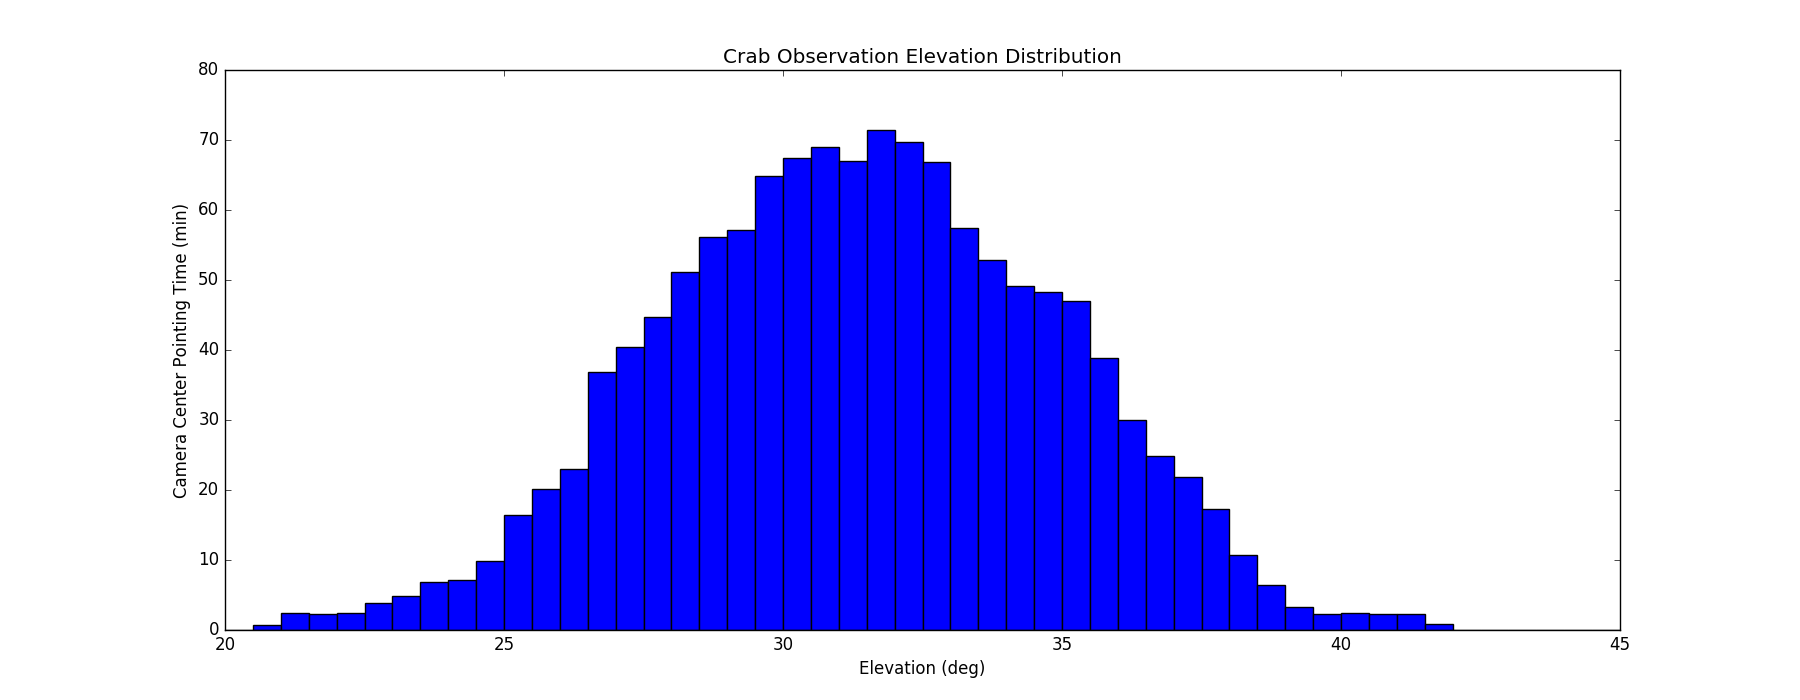
\includegraphics[width=0.95\textwidth]{images/halo_flux/plot.pdf}
    \caption[Galactic Center Halo J-factor Skymap]{
      J-factor of the dark matter halo model used in this analysis.
      The green circles indicate the different observation regions.
      Note this is showing the same model as Figure~\ref{fig:gchalo_jfactor}, except here the J-factor axis is linear instead of logarithmic.
      The black corners result from the halo model only being calculated out to a radius of \ang{3}, since there are no observations that extend past that.
    }
    \label{fig:halojfactor}
  \end{figure}

  The halo structure in Figure~\ref{fig:halojfactor} is a simple first step halo, one that does not account for more complex dark matter models.
  For example, a search for decaying dark matter would instead change the J-factor calculation to $\int \rho \, dl$, spreading out the gamma-ray emission.
  More exotic WIMP models may slightly alter the gamma-ray brightness of the dark matter halo, compared to the previously mentioned WIMP model.
  For example, if dark matter WIMPs have an attractive force between them, their effective annihilation cross section is enhanced, increasing the gamma-ray emission from the halo.
  This effect is called Sommerfeld enhancement~\cite{sommerfeld}.
  The dark matter search in this thesis {\color{red}does not include this effect (is there a reason not to include this?? -maria)}.
  % originally from http://inspirehep.net/record/1286230/files/Thesis-2009-Nierop.pdf
  % from http://www.pnas.org/content/112/40/12264.full.pdf
    
  
  \FloatBarrier
  
    
  \subsection{Spectrum of Gamma Rays from Dark Matter}\label{dm_spectral}
    In order to calculate the gamma-ray brightness of the dark matter halo, the produced spectrum from each WIMP annihilation must be known.
    Each WIMP annihilation can have distinct outcomes (each producing different pairs of particles), referred to as annihilation channels.
    WIMPs may annihilate directly into two gamma rays (the $\gamma\gamma$ channel), or may instead produce a quark-antiquark pair ($b\bar{b}$, $t\bar{t}$, ...), a lepton-antilepton pair, or {\color{red}almost (why almost?? -maria)} any other standard model particle-antiparticle pair.

    Non-gamma-ray annihilation channels may still indirectly produce gamma rays as the original particle pair decays.
    {\color{red}Many (why many?? -maria)} standard model interactions also result in a mix of channels, where the same interaction may produce different sets of particles with different probabilities, so WIMP annihilations may also have this feature.
    For an example set of 100 WIMP annihilation pairs, 80 pairs may annihilate into a $t\hat{t}$ pair, but then another 10 pairs may annihilate into a $b\hat{b}$ pair, and the remaining 10 pairs annihilate into other standard model particles.
    {\color{red}(where do you get these numbers/probabilities from?? -maria)}
    However, these mixed-channel searches are beyond the scope of this analysis.
    The software package CLUMPY~\cite{CLUMPYcode} is used in this thesis to calculate the gamma-ray spectra for each annihilation channel.
    The spectral models that CLUMPY uses are based on the annihilation spectra in the PPPC 4 DM ID~\cite{pppc4_dm_spectra,pppc4_ewcorrections}.
    These spectra are calculated using monte carlo simulations performed with PYTHIA~\cite{pythia} and HERWIG~\cite{herwig}.
    For this analysis, only the $b\bar{b}$ annihilation channel is considered.
    Figure~\ref{fig:chichi_spectrum} shows the resultant spectra from the single annihilation of two WIMPs.
    Each line shows the spectrum from a different initial WIMP mass.

    \begin{figure}[ht]
      \centering
      \includegraphics[width=0.95\textwidth]{images/spectra/chichi_spectrum.pdf}
      \caption[Single Annihilation Spectra]{
        Resultant photon spectra from the annihilation of two WIMP particles purely into the $b\bar{b}$ channel.
        Each colored line represents a different WIMP mass.
      }
      \label{fig:chichi_spectrum}
    \end{figure}

    These spectra can be combined with the J factor Equation~\ref{eqn:jfactor} to calculate Equation~\ref{eqn:dmflux}: the number of gamma rays produced by the halo
    It is important to note that mass-to-light ratios, and their derived J factors are usually inferred from measuring star spectra.
    These measured J factors can suffer from large errors, as it can be difficult to determine which stars are within a target gravitational well, and which ones are foreground or background stars~\cite{segue_jfactor_errors}.
    
    Using some estimated parameters with Equation~\ref{eqn:dmflux}, the flux of gamma rays from a dark matter halo can be estimated to understand how few events a dark matter halo produces.
    For this estimate, the dark matter mass is chosen to be \SI{10}{TeV}, and the velocity-averaged cross section $\left < \sigma v \right >$ is set at the relic cross section.
    Other chosen parameters are specified in Table~\ref{tab:halo_nphotons}, to align with the VERITAS telescope performance, or the parameters of the dark matter analysis performed in later chapters.
    For the table parameters, the dark matter halo would only produce a VERITAS-detectable gamma ray between \SIrange{4}{70}{TeV} every 39 hours.
    This flux $\Phi$ is proportional to the $\sv$, so a factor of $n$ larger particle cross section would produce a factor of $n$ larger photon flux.
    It is interesting to note that, if the entire VERITAS energy range of \SIrange{1.5}{70}{TeV} is used, the integrated photon spectrum increases to 0.13 events per annihilation, increasing the observed photon flux by a factor of 26.
    
    \begin{table}[]
      \centering
      \begin{tabular}{r|l}
        \hline
        \textbf{Estimated Parameters}            & \\
        $m_{\chi}$                               & \SI{10}{TeV}         \\
        relic cross section $\left < \sigma v \right >$        & \SI{3e-26}{cm^3/s}   \\
        Field of View                            & \ang{3}              \\
        Detectable Photon Energy Range           & \SIrange{4}{70}{TeV} \\
        Observatory Effective Area               & \SI{287000}{m^2}     \\
        Annihilation Branch                      & $\chi\chi \rightarrow b\bar{b}$ \\
        DM Halo Shape                            & Einasto              \\
        \hline
        \textbf{Derived Values}                  & \\
        Integrated Photon Spectrum : $\int \frac{dN_{\gamma}}{dE} dE$        & 0.00536 photons per $\chi\chi$ annihilation \\
        J factor :$\int \int \rho^2 dl\,d\Omega$ & \SI{3.88e22}{GeV^2/cm^5}      \\
        Halo Flux $\Phi$                         & \SI{2.5e-11}{photons/(s*m^2)} \\
        One halo photon detected every           & \SI{39}{hours} \\
        \hline
      \end{tabular}
      \caption[Halo Model Parameters]{
        Number of Gamma Rays from a Dark Matter Halo.
        Field of view is the radial field of view of VERITAS.
        Observatory Effecitve area is the VERITAS effective area at \ang{28} telescope elevation (average elevation of Galactic Center at VERITAS's latitude), \ang{0.5} offset from GC, at the $\log_{10}$ mean energy (\SI{16.7}{TeV}) in the selected energy range.
        The Einasto halo shape parameters are chosen to be the same as in Section~\ref{dm_spatial}.
      }
      \label{tab:halo_nphotons}
      % values derived with $VERIPY/thesis/analysis/example_dm_halo_photons/example.py
    
    \end{table}

    \FloatBarrier
    
\section{Cherenkov Photons}\label{sec:cherenkov}

  Because the detection of gamma rays in Section~\ref{sec:atmoshowers} relies heavily on knowledge of Cherenkov light, Cherenkov light and its production is discussed here.
  Within the Earth's atmosphere (or any dielectric medium), the phase velocity of light $c_{atmosphere}$ is slightly slower than in a vacuum.
  Any charged particles travelling at velocity $v > c_{atmosphere}$ will induce the atmosphere to produce Cherenkov photons~\cite{cherenkov}.
  From a single charged particle of constant velocity, Cherenkov photons form a conical wavefront shown in Figure~\ref{fig:cherenkovangle}.
  This wavefront is similar to a sonic boom shockwave, or the wake produced when a boat travels faster than the speed of the waves.

  \begin{figure}[ht]
    \centering
    \includegraphics[width=0.27\textwidth]{images/cherenkov_angle/cherenkovangle.pdf}
    \caption[Chernekov Emission Angle]{
      Cherenkov light (blue arrows) is emitted at angle $\theta$, relative to the charged particle z's path.
    }
    \label{fig:cherenkovangle}
  \end{figure}

  Cherenkov photons are produced at an angle $\theta$ relative to the charged particle's path, determined by the index of refraction of the medium $n$, the speed of the charged particle $v$, and the speed of light in the medium $c$, as in Equation~\ref{eqn:cherenkovangle}.
  For the air showers used in this analysis, the Cherenkov angle $\theta$ is \nicetilde\ang{1}.
  % showers are 10km up, light pool on ground is 130m diameter, \theta = ArcSin(130/10000) * 180 / pi = 0.73deg ~ 1deg

  \begin{equation}\label{eqn:cherenkovangle}
    \theta = ArcCos \left ( \frac{c}{n \; v} \right )
  \end{equation}
  
  In practice, air showers are more complex due to the number and distribution of charged particles and their velocities, as well as energy losses.
  These effects tend to smear the theoretically-clean Cherenkov cones into a diffuse pool of light on the ground, shown in Figure~\ref{fig:lightpool}.

  \begin{figure}[ht]
    \centering
    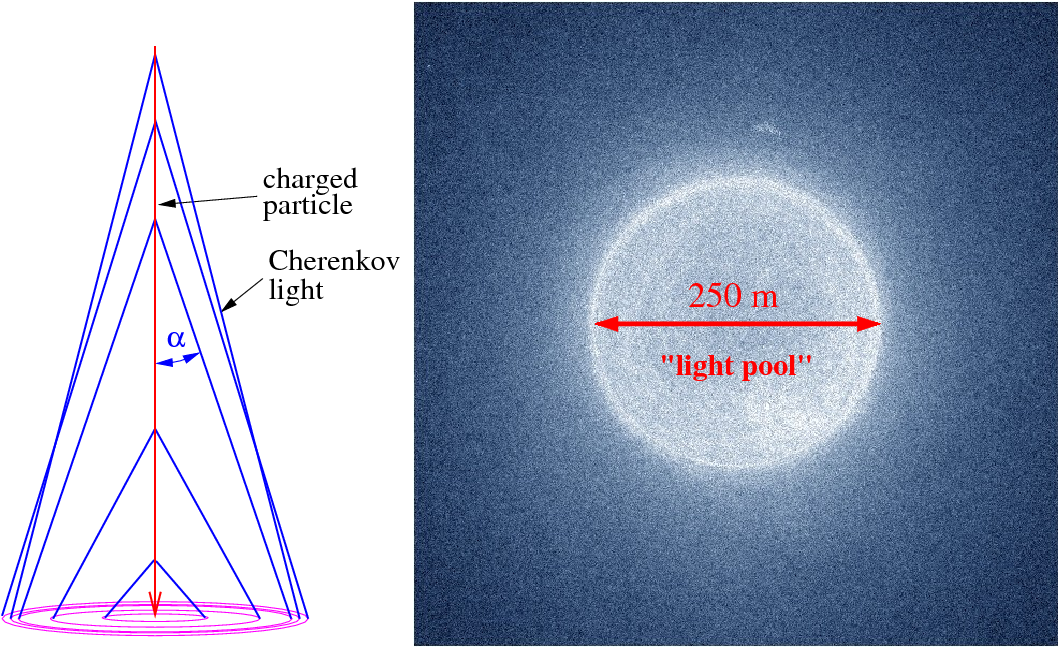
\includegraphics[width=0.85\textwidth]{images/lightpool/lightpool.pdf}
    \caption[Chernekov Light Pool]{
      Cherenkov light from a gamma ray shower illuminating the ground.
      Due to the changing atmospheric density, the Cherenkov angle changes as the electromagnetic shower decends (Left), concentrating the emitted light into a ring-like pool (Right).
      The initial gamma ray had an energy of \SI{1}{\TeV}.
      Figure is from Ref.~\cite{Voelk}.
    }
    \label{fig:lightpool}
  \end{figure}
  
  The spectrum of photons produced by the Cherenkov effect can be calculated with the Frank-Tamm formula~\cite{franktamm1,franktamm2} in Equation~\ref{eqn:franktamm},
  
  \begin{equation}\label{eqn:franktamm}
    \frac{dE}{dx\,d\omega}=\frac{(ze)^2 \, \omega}{c^2} \left ( 1 - \frac{c^2}{v^2 \;\epsilon(\omega)} \right )
  \end{equation}
  
  where $E$ is the energy emitted as Cherenkov radiation, $x$ is the length of the charged particle path, $ze$ is the charge of the particle, $\omega$ is the emitted Cherenkov photon frequency, $c$ is the speed of light (phase velocity) in the medium, $v$ is the speed of the particle, and $\epsilon(\omega)$ is the frequency-dependent permittivity.
  
  \begin{figure}[ht]
    \centering
    \includegraphics[width=0.75\textwidth]{images/CherenkovReactor/cherenkovreactor.eps}
    \caption[Chernekov Light from a Reactor]{
      Blue Cherenkov light in the Advanced Test Reactor core, at the Idaho National Laboratory~\cite{cherenkovreactor,atrlab}.
    }
    \label{fig:cherenkovreactor}
  \end{figure}
  
  In Figure~\ref{fig:cherenkovreactor}, a visible example of Cherenkov photons is shown, produced in the Advanced Test Reactor at the Idaho National Laboratory.
  Neutrons emitted by the reactor collide with atoms in the water, freeing some electrons with enough kinetic energy to travel faster than the speed of light in water.
  These superluminal-in-water electrons then create the blue Cherenkov photons imaged here.
  
  Now that it is understood that Chernekov light is produced by charged particles, the next Section~\ref{sec:atmoshowers} discusses how particles from outer space can produce waves of Cherenkov photons.
  These UV- and visible-spectrum Cherenkov photons are then imaged and recorded by the VERITAS observatory, discussed in Chapter~\ref{chapter:veritas}.
  {\color{red}(this is a good transition paragraph, add more between the other subsections?? -maria)}
  
    
\section{Atmospheric Showers}\label{sec:atmoshowers}

  When a particle strikes an atom of Earth's atmosphere at GeV or higher energies, it sets off a cascade of energetic particles called an air shower~\cite{Bethe1934,Klein1999}.
  When the primary particle is composed of one or more hadrons, like a proton or iron atom, it creates a hadronic shower.
  When the primary is a gamma ray or a charged lepton, it creates an electromagnetic shower.
  Electromagnetic showers produce a cascade of $e^{\pm}$s and $\gamma$s, where each successive generation of particles tends to have more particles but less energy per particle than the last.
  {\color{red}(did $e^{\pm}$ and $\gamma$ get defined before?? -maria)}
  To start the shower, the primary gamma ray will interact with an atmospheric atom, producing an $e^{-}e^{+}$ pair, each with roughly half the primary gamma ray's energy, as shown in Figure~\ref{fig:emcascade}.
  The $e^{-}$ and $e^{+}$ emit bremsstrahlung photons, and incite the atmosphere to emit Cherenkov photons.
  Cherenkov photon production is discussed further in Section~\ref{sec:cherenkov}.
  The higher-energy bremsstrahlung photons then produce $e^{-}e^{+}$ pairs, which go on to produce more bremsstrahlung and Cherenkov photons.
  As each newly created particle has less energy than its parent particle, eventually the particles in the shower don't have enough energy to produce additional child-particles.
  When electrons have around \SI{80}{MeV}\footnote{This is the energy where, for an electron, the loss of energy due to ionization is equal to the loss of energy due to bremstrahlung~\cite{tanabashi2018review,berger196410}} or less of kinetic energy, energy losses due to ionization begin to dominate~\cite{pdg_2014}.

  \begin{figure}[ht]
    \centering
    \includegraphics[width=0.95\textwidth]{images/cascade_diagram/feynman/cascade.pdf}
    \caption[Electromagnetic Cascade]{
      Diagram of the first few generations of an electromagnetic cascade as it decends downwards through the atmosphere, layered by interaction generation~\cite{ellis2017tikz}.
      At the top of the diagram, $\gamma{}_o$ is the initial astrophysical gamma ray.
      \CaptionBlankLine
    }
    \label{fig:emcascade}
  \end{figure}

  Of all detected air showers, \nicetilde{}99\% are due to protons and electrons, rather than gamma rays.
  {\color{red}(why so many more protons and electrons than gamma rays?? -maria)}
  Protons produce hadronic showers which also produce Cherenkov light, like electromagnetic showers.
  In the initial collision, the astrophysical proton $p_{\textrm{cosmic}}$ interacts with an atmospheric proton $p_{\textrm{atmo}}$.
  The proton-proton collision then produces a set of pions, as in Equation~\ref{eqn:protoncollision}, as well as other particles (`$...$') whose production rates vary with available interaction energy.
  These other particles include additional protons, neutrons, and other hyperons, as well as kaons, other mesons, and additional nucleons.
  These all go on to interact and decay to produce further particles, as part of a hadronic cascade.
  
  \begin{equation}\label{eqn:protoncollision}
    p_{\textrm{cosmic}} + p_{\textrm{atmo}} \rightarrow \pi^+ + \pi^+ + \pi^0 + ...
  \end{equation}
  
  The cascade also creates electrons, positrons, and photons, so after each generation of the cascade, roughly 1/3 of the hadronic shower's energy is transferred into a new electromagnetic sub-shower.
  The interaction produces $\pi^+\pi^+\pi^0$, where each particle receives \nicetilde $\frac{1}{3}$ of the initial proton's energy.
  This $\pi^{0}$ decay is shown in Figure~\ref{fig:feynman_pi0}.
  
  \begin{figure}[ht]
    \centering
    \includegraphics[width=0.5\textwidth]{images/feynman_particles/pion_gamma.pdf}
    \caption[Feynman Diagram of $\pi^{0}$ Decay]{
      Feynman diagram of a $\pi^{0}$ decaying into two photons.
      \CaptionBlankLine
    }
    \label{fig:feynman_pi0}
  \end{figure}

  \begin{figure}[ht]
    \centering
    \includegraphics[width=0.5\textwidth]{images/feynman_particles/pionplus.pdf}
    \caption[Feynman Diagram of $\pi^{+}$ Decay]{
      Feynman diagram of $\pi^{+}$ decaying into a lepton pair.
      \CaptionBlankLine
    }
    \label{fig:feynman_piplus}
  \end{figure}
  
  In order to accurately measure the gamma rays from an astrophysical source, the hadronic showers must first be removed.
  Because hadronic showers produce a slightly different image of Cherenkov light, many of them can be excluded from the analysis.
  The process of identifying and excluding these hadronic showers is referred to as gamma-hadron separation.

  % see here for neutron: https://en.wikipedia.org/wiki/Cosmic_ray
  In hadronic showers, any produced \pip{}'s and \pim{}'s can travel far in the tranverse direction, away from the main axis of the primary particle.
  The \pip{}'s and \pim{}'s then decay into $\mu^{+}\nu_{\mu}$ and $\mu^{-}\bar{\nu}_{\mu}$ pairs, respectively.
  The \pip{} decay is shown in Figure~\ref{fig:feynman_piplus}.
  The \pio{} quickly decays into pair of gamma rays, each of which then start their own electromagnetic shower.
  The \pip{} and \pim{} have longer decay times ($\pi^{\pm} \rightarrow $\SI{3e-8}{s} vs $\pi^{0} \rightarrow $\SI{9e-17}{s}~\cite{pdg_2014}), allowing them to carry energy farther away from the central shower axis.
  Both of these effects create sub-showers farther away from the primary particle axis, which tends to cause hadronic showers (and their resulting Cherenkov images, discussed in Section \ref{sec:cherenkov}) to be wider than a purely electromagnetic shower of the same length. 
  
  In Figure~\ref{fig:gamma_vs_proton_airshower}, the differences between a gamma-ray shower (left) and a proton shower (right) are shown.
  In the figure, darker areas indicate more Cherenkov photons are produced by charged particles in the shower.
  The gamma-ray shower produces most of its Cherenkov photons along the vertical core of the shower, while the proton shower produces Cherenkov photons spread out in a wider, fan-like shape.
  The initial energies were chosen as such because a \SI{1}{TeV} proton will on average divest $\frac{1}{3}$ of its energy to the \pio{}.
  This means that the gamma-ray and the proton-produced-pion start with the same amount of available energy, and that both showers produce similar amounts of Cherenkov light.
  The \pio{} then decays into the electromagnetic sub-shower in the interior of the proton shower.
  The net effect is that, when compared to a gamma ray, a proton must start with 3 times the energy to produce a similar amount of Cherenkov photons, which are distributed in a wider pattern.

  \begin{figure}[ht]
    \centering
    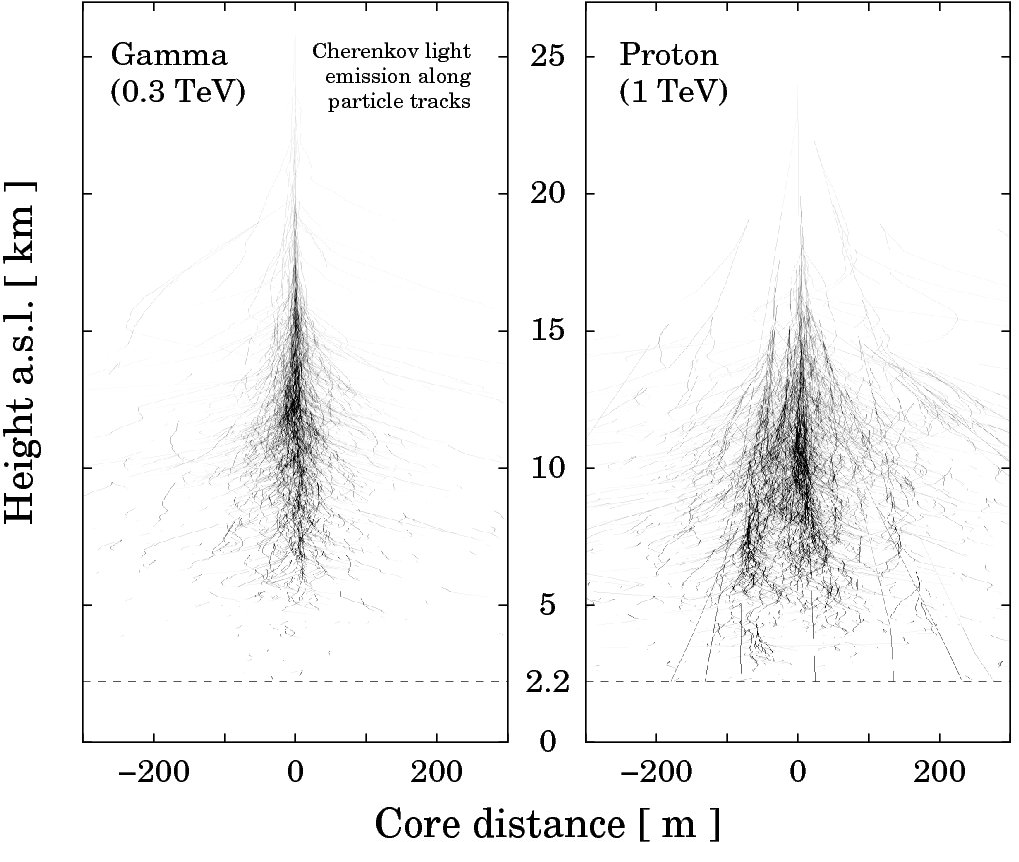
\includegraphics[width=0.95\textwidth]{images/showers_gamma_proton}
    \caption[Gamma Ray and Proton Showers]{
      A gamma ray shower (left) alongside a proton shower (right)~\cite{Bernlohr2008149}.
    }
    \label{fig:gamma_vs_proton_airshower}
  \end{figure}
  
  \FloatBarrier


\cleartooddpage[\thispagestyle{empty}]
\chapter{VERITAS}

\begin{figure}[h]
  \begin{center}
    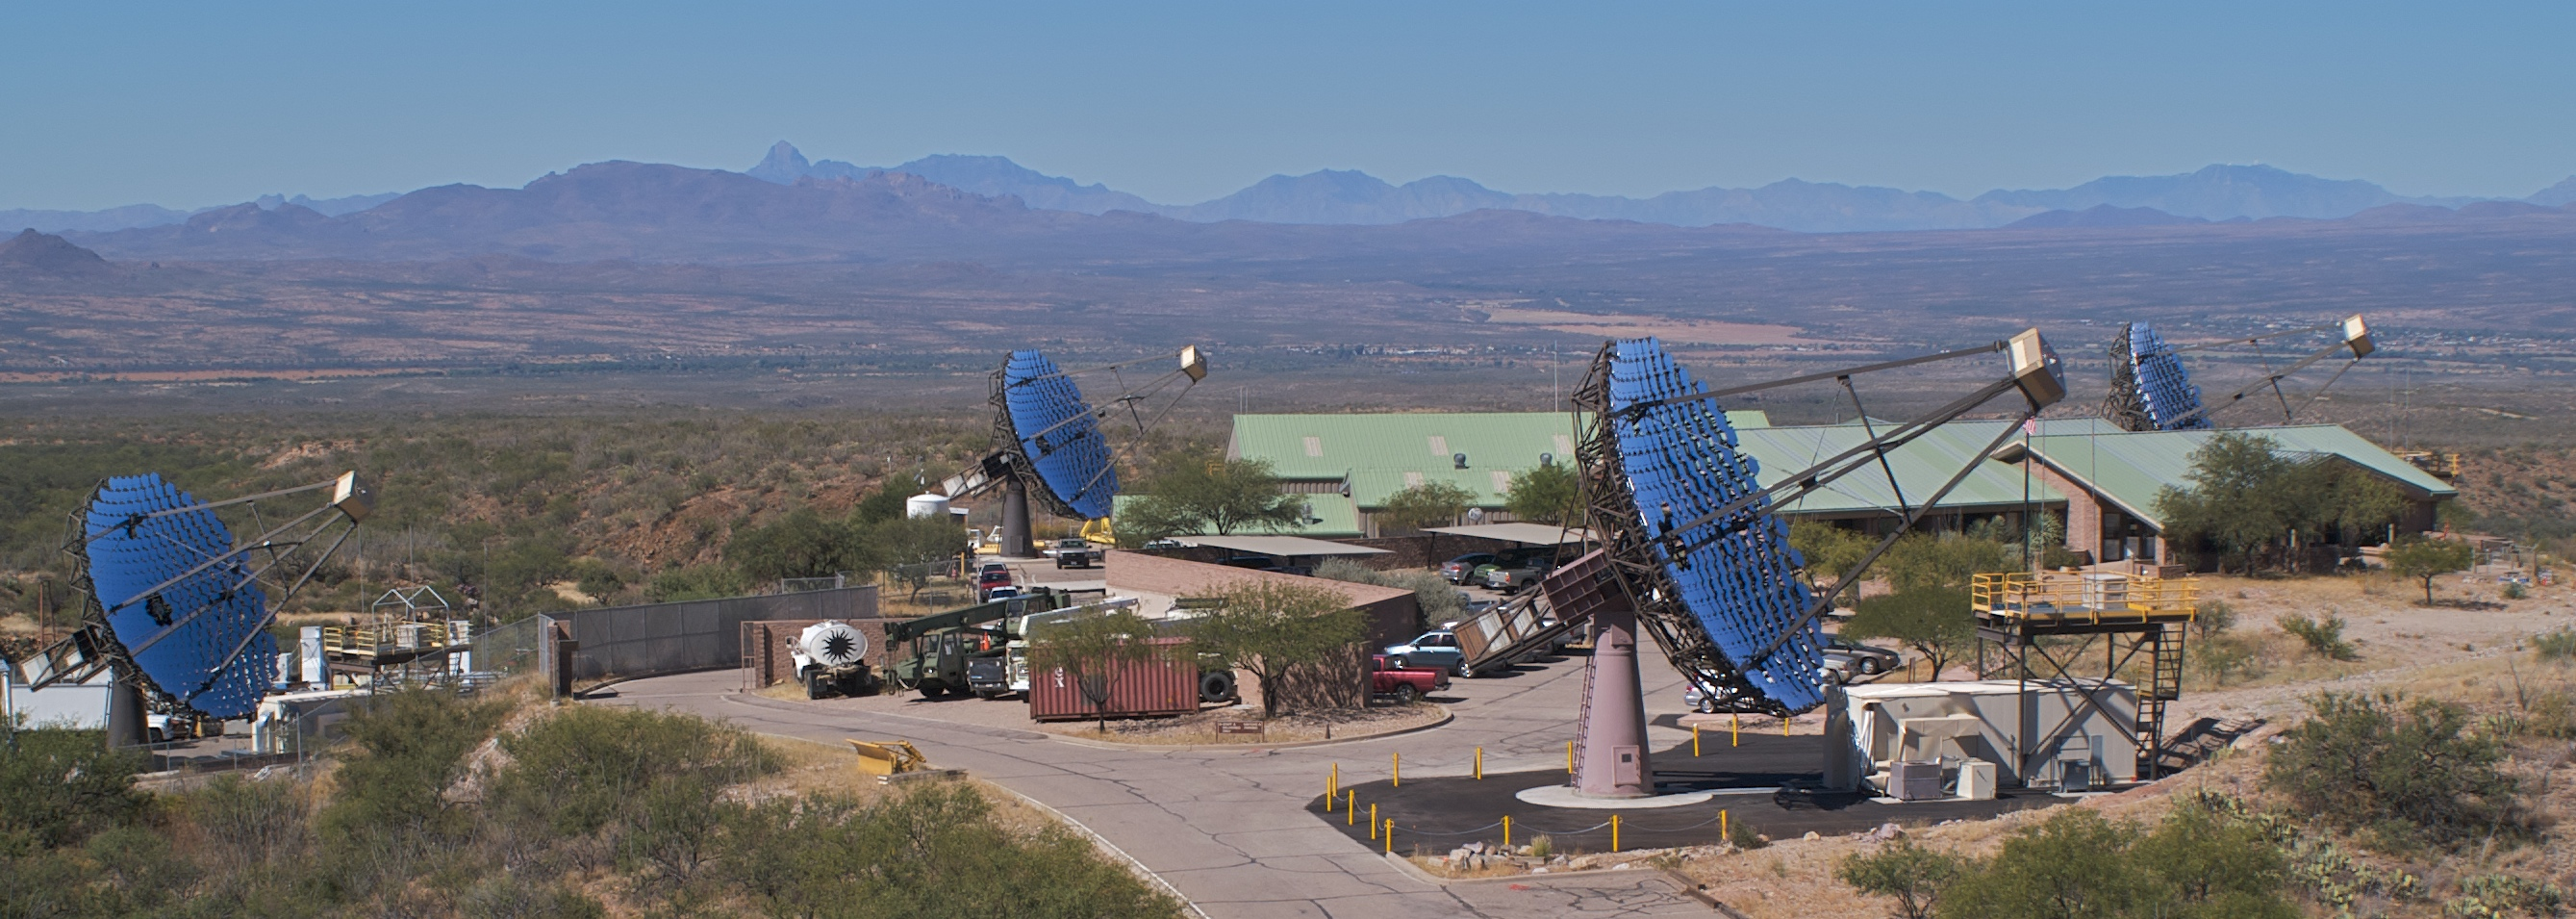
\includegraphics[width=0.95\textwidth]{images/veritas_array_v6}
    \caption[VERITAS Array]{The VERITAS observatory.}\label{fig:veritasarray}
  \end{center}
\end{figure}

VERITAS is a gamma ray observatory operating in Arizona, USA, capable of detecting $\nicetilde$TeV-energy gamma rays.
This detection is performed by an array of four Imaging Atmospheric Cherenkov Telescopes, each spaced $\nicetilde$50m apart.
Each telescope possesses an array of 345 mirrors, and a Photomultiplier Tube (PMT) camera (containing 499 PMTs) on a set of struts.
When a gamma-ray produces an air shower in the atmosphere, the shower emits blue-UV Cherenkov photons over a timespan of nanoseconds.
By focusing these photons onto the PMT camera with the mirrors, images of the shower can be taken, where each pixel of the image consists of analog voltage pulses from each PMT, with more photons causing larger pulses.


%As the width of voltage pulses must be \nicetilde{}ns to prevent overlapping with the pulses from other showers, the digization hardware measures the time-dependent voltage of each pulse in 1-nanosecond-wide(??) time bins.
%Though faint showers may only posess a few photons per PMT, brighter showers can still shine several thousand photons onto individual pixels.
%This means that the digization hardware must be able to handle a large dynamic range of inputs, over several orders of magnitude in voltage.
%To accomplish this, two amplification levels are used in the digization circuit, High Gain for voltage pulses of a few photons, and Low Gain for voltage pulses of several thousand photons.

In the following sections, the different hardware components are examined, in order of signal propagation.
In section \ref{sec:telpoint}, the Telescope Pointing is discussed, including its monitoring and calibration.
The Mirrors are discussed in section \ref{sec:mirrors}, including their properties and alignment.
In section \ref{sec:pmts}, the PMTs are discussed, including their performance and calibration.
The trigger system is discussed in section \ref{sec:trig}, relating how candidate signal voltages are saved while discarding those sourced from noise.
In section \ref{sec:epochs}, the different observatory epochs are discussed, as over time changes and modifications have changed the observatory's performance.


\section{Telescope Pointing}\label{sec:telpoint}

\begin{figure}[h]
  \begin{center}
    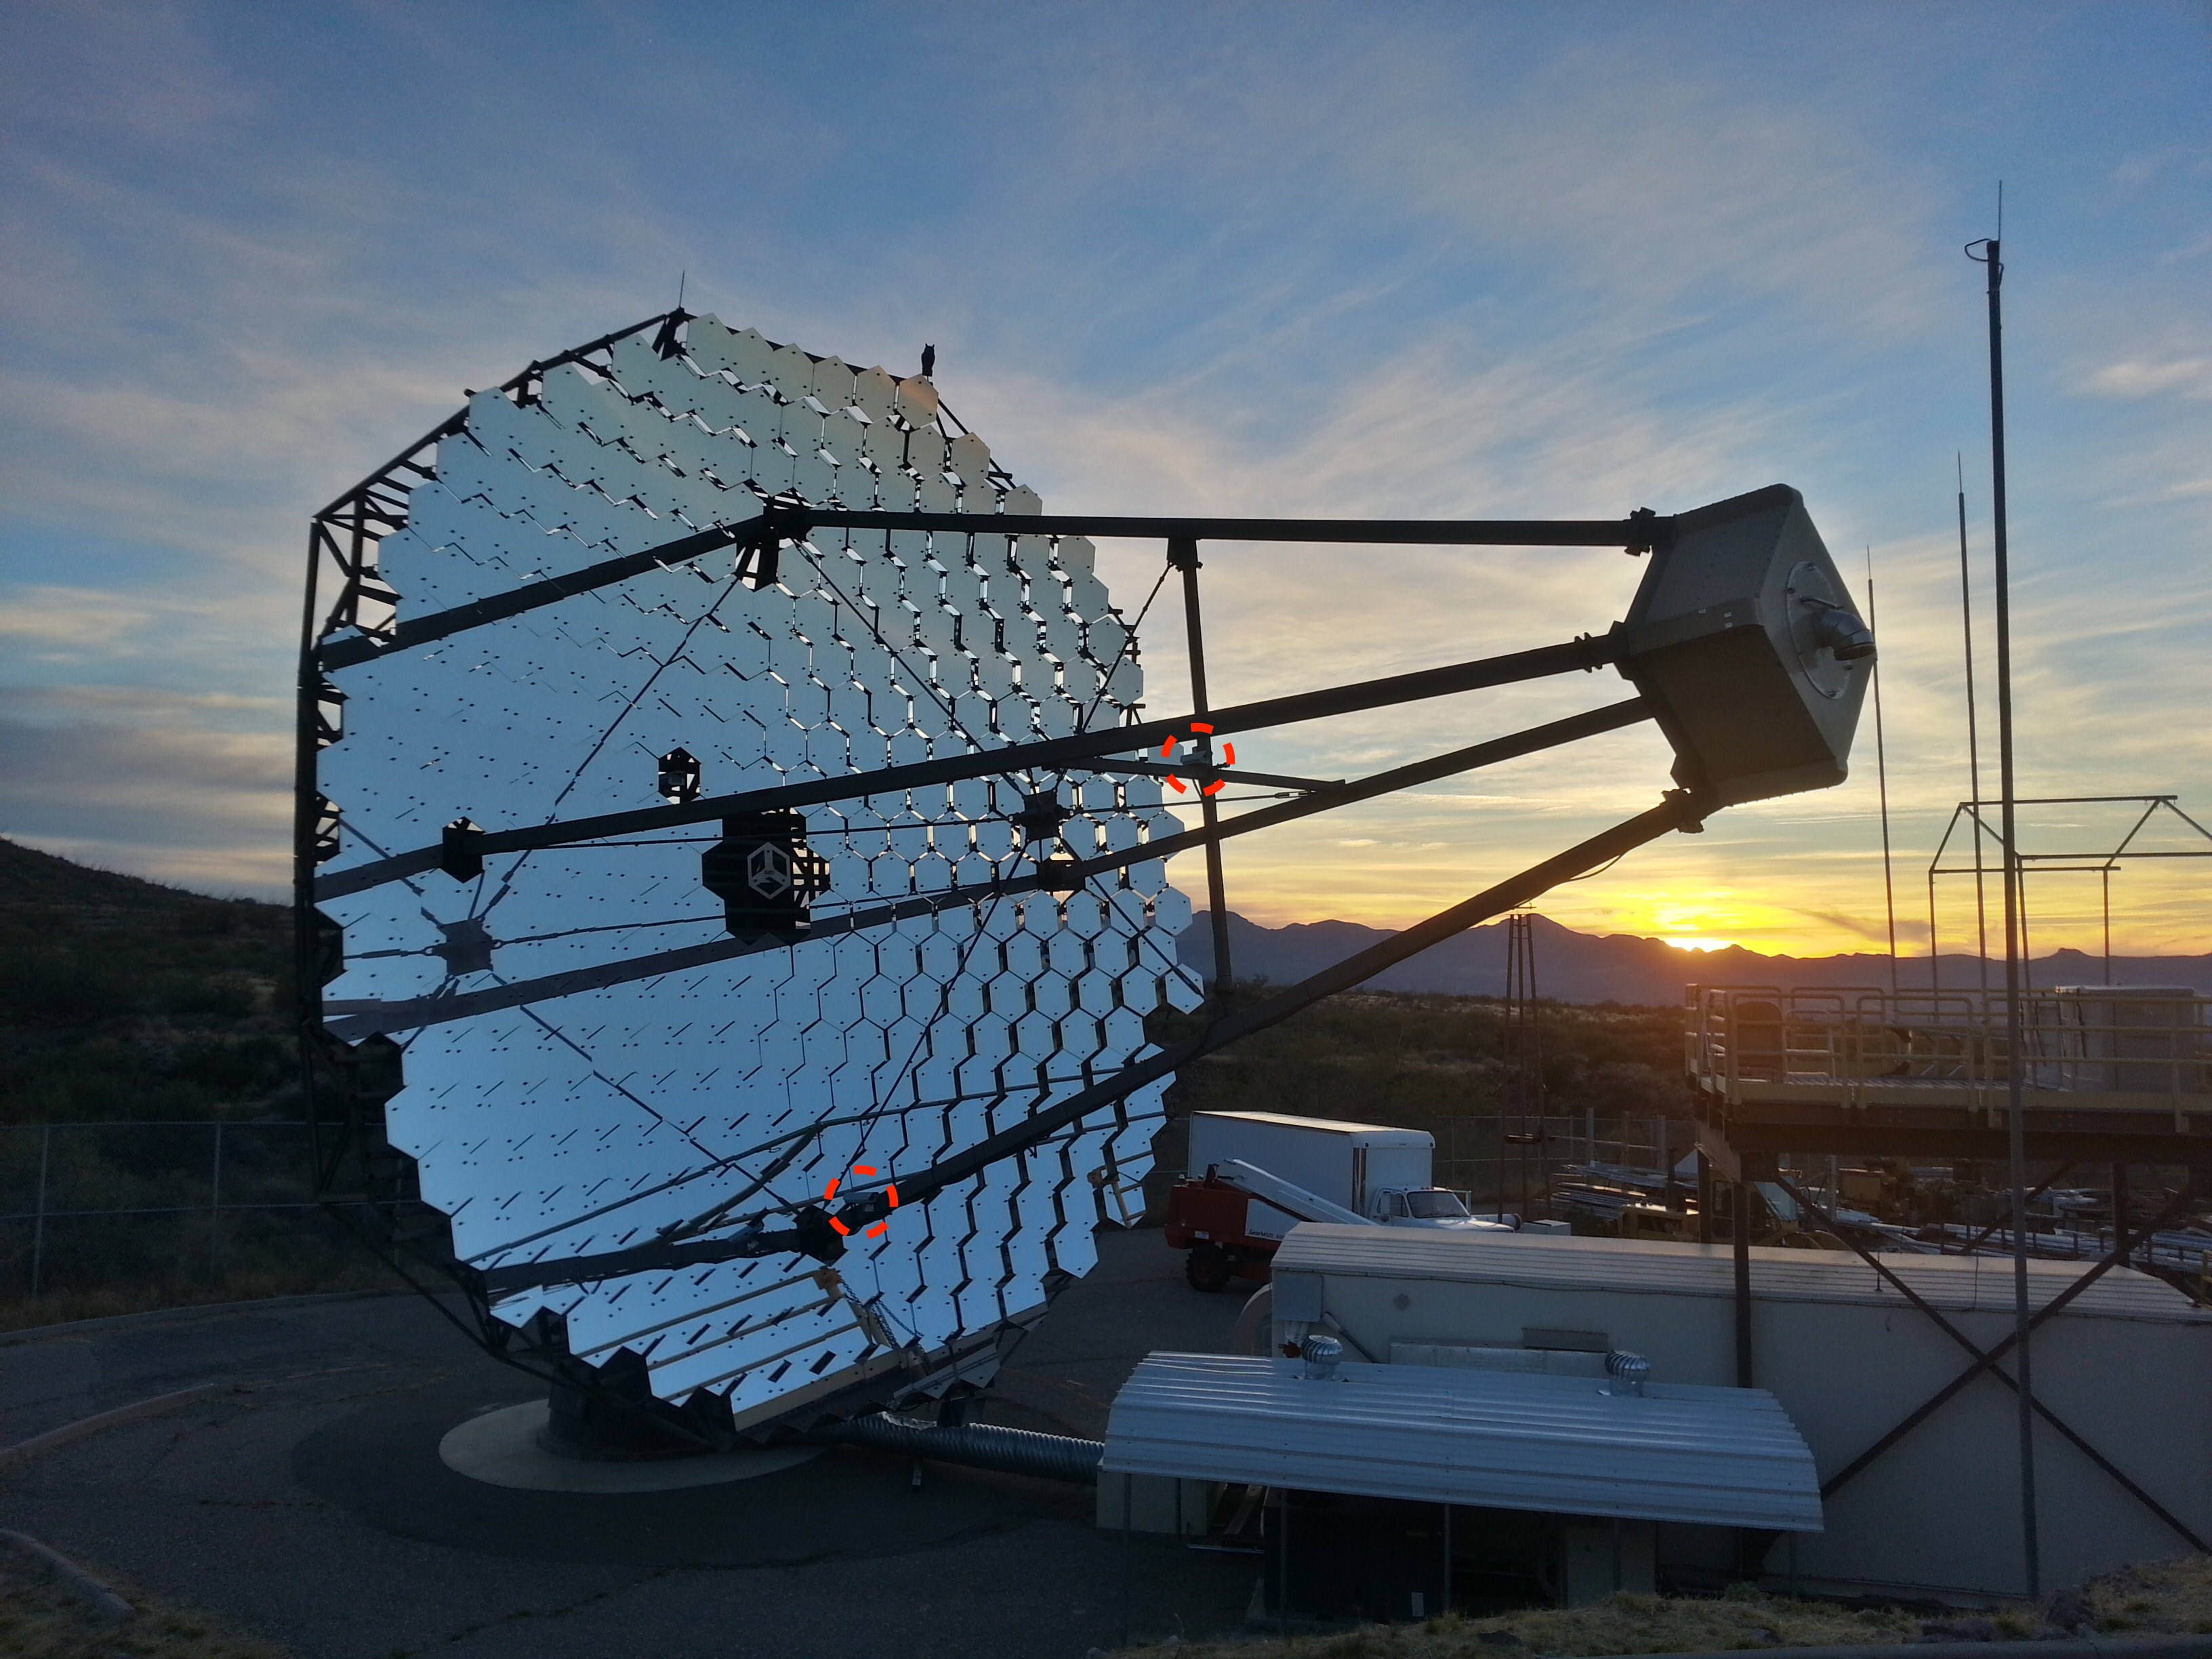
\includegraphics[width=0.95\textwidth]{images/single_telescope}
    \caption[Single Veritas Telescope]{View of the 345 mirrors, the support structure, and the PMT Camera housing at the end of the four supporting arms.}\label{fig:davcottel}
  \end{center}
\end{figure}

Like most telescopes, each VERITAS telescope has an immobile base, and a pointable dish for collecting light.
This dish can rotate in azimuth and in elevation, with enough range in both axes to point at any direction above the horizon.
At their fastest, the telescopes can slew at a rate of $\nicetilde$1\degree per second.
To track where the telescopes are pointing, the motors that drive the azimuth and elevation movement have encoders that digitize the pointing direction of the dishes.
However, as the dishes are large metal structures, they bend and flex at different elevations and azimuths.
To account for this flexing, the encoder values are then given to a structural model (??), which accounts for the dish structure bending at different azimuths and elevations.
After applying this model, the telescope pointing can be tracked with an accuracy of 0.013\degree to 0.027\degree \cite{Veritas_Detector}.

As an improvement to the encoder measurement, a Virtual Pointing Monitor (VPM) system is also in place.
The VPM consists of two CCD cameras fixed to each telescope, pointing parallel to the telescope pointing, and a set of LED lights attached to the camera, next to the Winston cones (see section \ref{sec:pmts}).
The first CCD camera is attached below the bottom mirrors, and images the stars in the field of view.
The second CCD camera is attached to the support struts, roughly halfway between the mirrors and the camera, and images the focal plane of the telescope.
Both cameras are visible in figure \ref{fig:davcottel}
During regular observations, these cameras take images of the background stars and the focal plane every two seconds, and (??), resulting in an improved pointing accuracy of \nicetilde 0.0069\degree (originally in griffen thesis 2016, pg45, but is there a better citation??).

As the VERITAS telescopes are based on old designs for a military solar concentrator that sets targets on fire\cite{daviescotton}, the VERITAS telescopes have similar abilities.
This mostly means that care must be taken during the day to point the telescopes away from the sun during maintanance and storage.
% 100m^2 * 1000w/m^2 = 100,000W
If any direct sunlight falls onto the telscope mirrors, the \nicetilde100,000 Watts of light will be concentrated either onto the camera, or a point within a few meters of the camera, which could potentially cause signficant damage to telescope hardware or nearby plants, animals, and people.
VERITAS telescopes are stored during the day by pointing them at \nicetilde0\degree elevation, North.


\section{Mirrors}\label{sec:mirrors}

When cherenkov light first interacts with the telescope array, it is by being reflected by one of 345 mirrors.
These mirrors face towards the incoming cherenkov light, with the PMTs positioned in a camera box, facing the mirrors, shown in figure \ref{fig:davcottel}.
This configuration is referred to as a Davies-Cotton telescope \cite{daviescotton}.
Each mirror has an area of 0.322$m^2$, and a spherical curvature radius of 24m.
The mirrors are each mounted along the support structure so that the total diameter of the telescope mirror area is 12m, with a focal length of 12m, and a total mirror area of 111$m^2$ \cite{Veritas_Detector}.
The mirrors' reflectivity as a function of wavelength is shown in figure \ref{fig:mirreflect}.

\begin{figure}[h]
  \begin{center}
    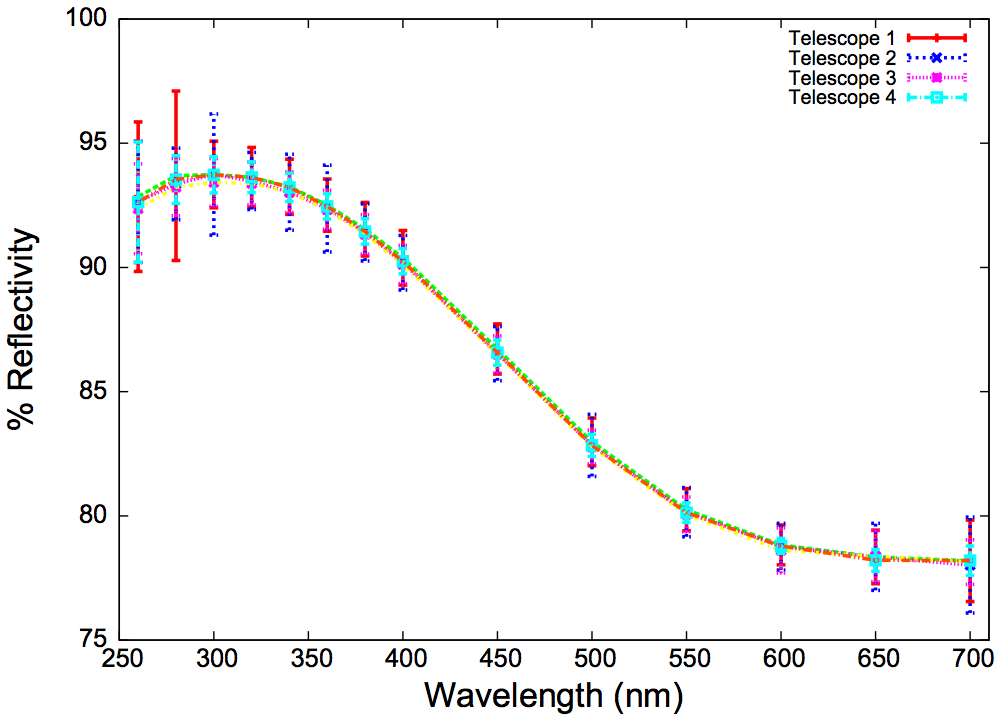
\includegraphics[width=0.75\textwidth]{images/mirror_reflect}
    \caption[Mirror Reflectivity]{Mirror reflectivity as a function of wavelength for each telescope, from \cite{mirrorfacets}.  The VERITAS specifications state that the mirror reflectivity must be $\geq 85\%$ between 280nm and 450nm.}\label{fig:mirreflect}
  \end{center}
\end{figure}

As the mirrors are exposed to the elements, they slowly accumulate dust and scratches.
To combat this, they are cleaned and recoated at regular (yearly??) intervals.
Each mirror is attached to the support structure via three adjustable mounting points, meaning the mirror orientation can be adjusted to point directly on the camera, detailed in \cite{mirroralign}.
This alignment is measured and adjusted at regular intervals, using background stars as a calibration source??.


\subsection{Star Point Spread Function}

By pointing a telescope at Polaris and placing a CCD at the focal plane, the mirror PSF can be measured.
This was done with the first VERITAS telescope was built, where the image is shown in figure \ref{fig:mirrorpolaris}.
The mirror psf is 0.06\degree full width half maximum\cite{Veritas_Detector}.

\begin{figure}[h]
  \begin{center}
    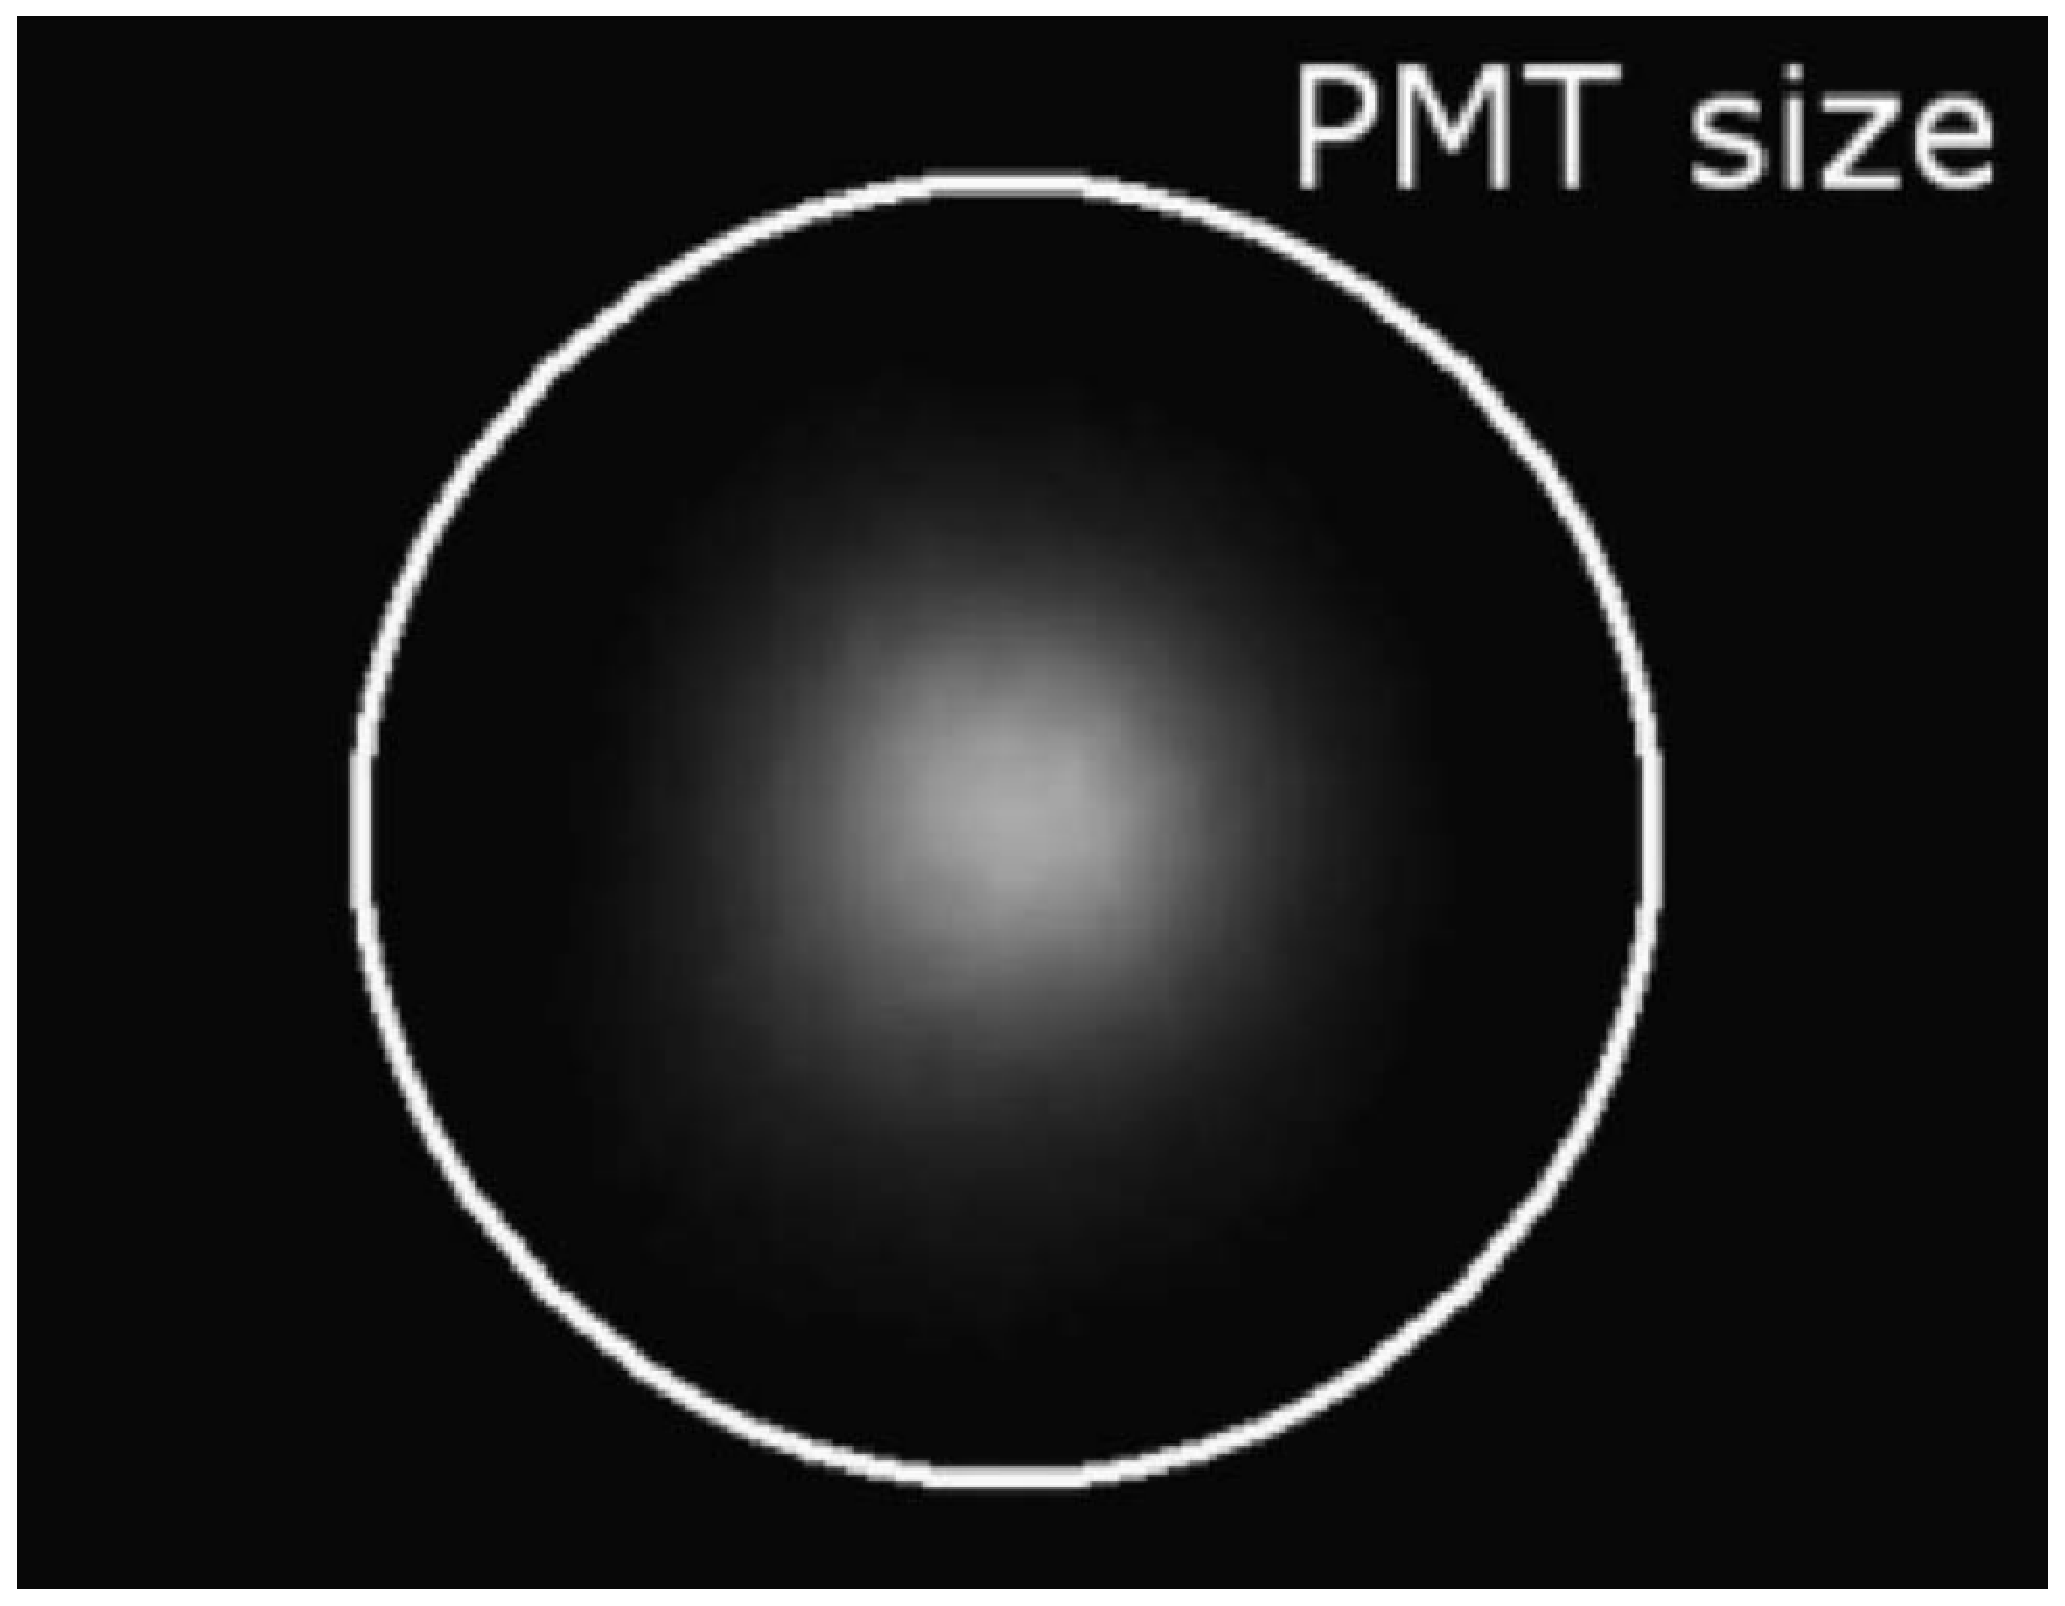
\includegraphics[width=0.75\textwidth]{images/mirror_polaris.eps}
    \caption[Polaris PSF]{Image of Polaris after reflecting off the mirrors, demonstrating the mirror Point Spread Function, from \cite{Veritas_Detector}.  The circle indicates the radius of a PMT.}\label{fig:mirrorpolaris}
  \end{center}
\end{figure}

\subsection{Mirror Alignment}
% https://veritas.sao.arizona.edu/wiki/index.php/Mirror_Alignment
The mirrors are each mounted to the dish on three adjustable mounting points.
By adjusting the mounting points, the mirrors can be individually aligned.
The alignment procedure is performed by placing a CCD camera at the focal plane, facing towards the mirrors.
The telescope is then pointed towards a magnitude 2 star at \nicetilde70\degree elevation.
The pointing is known as a 'raster' scan of the star, where each mirror's field of view is in turn centered on the star.
By using the CCD to examine the position of the star in each mirror, the mirror's alignment can be calculated and corrected.



\section{PMTs}\label{sec:pmts}

Each telescope has a PMT Camera on the end of four supporting arms, inside a protective housing.
This camera consists of 499 Photo Multiplier Tubes (PMTs), each with a Winston cone to increase the light collection area for each PMT.
The PMTs are Hamamatsu's model R10560-100-20 MOD \cite{pmtmodels}.
These winston cones can be seen attached to the PMTs in figure \ref{fig:winstcones}.

\begin{figure}[h]
  \begin{center}
    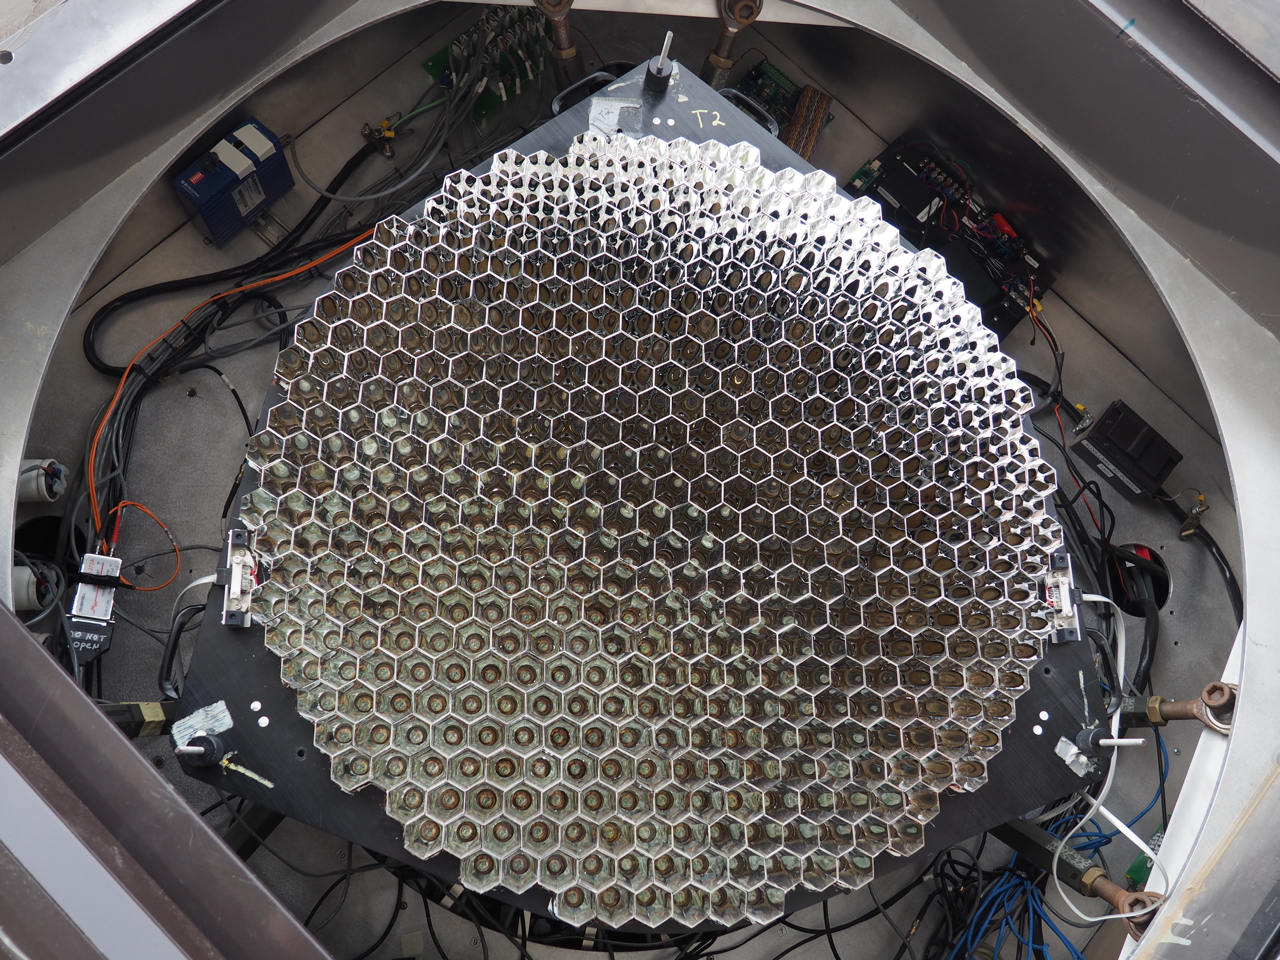
\includegraphics[width=0.75\textwidth]{images/winston_cones_t2}
    \caption[Winston Cones]{Hexagonal Winston cones over the circular PMTs, inside the camera housing.}\label{fig:winstcones}
  \end{center}
\end{figure}

To operate, the PMTs are connected to high voltage, which is typically around several hundred Volts.

\begin{figure}[h]
  \begin{center}
    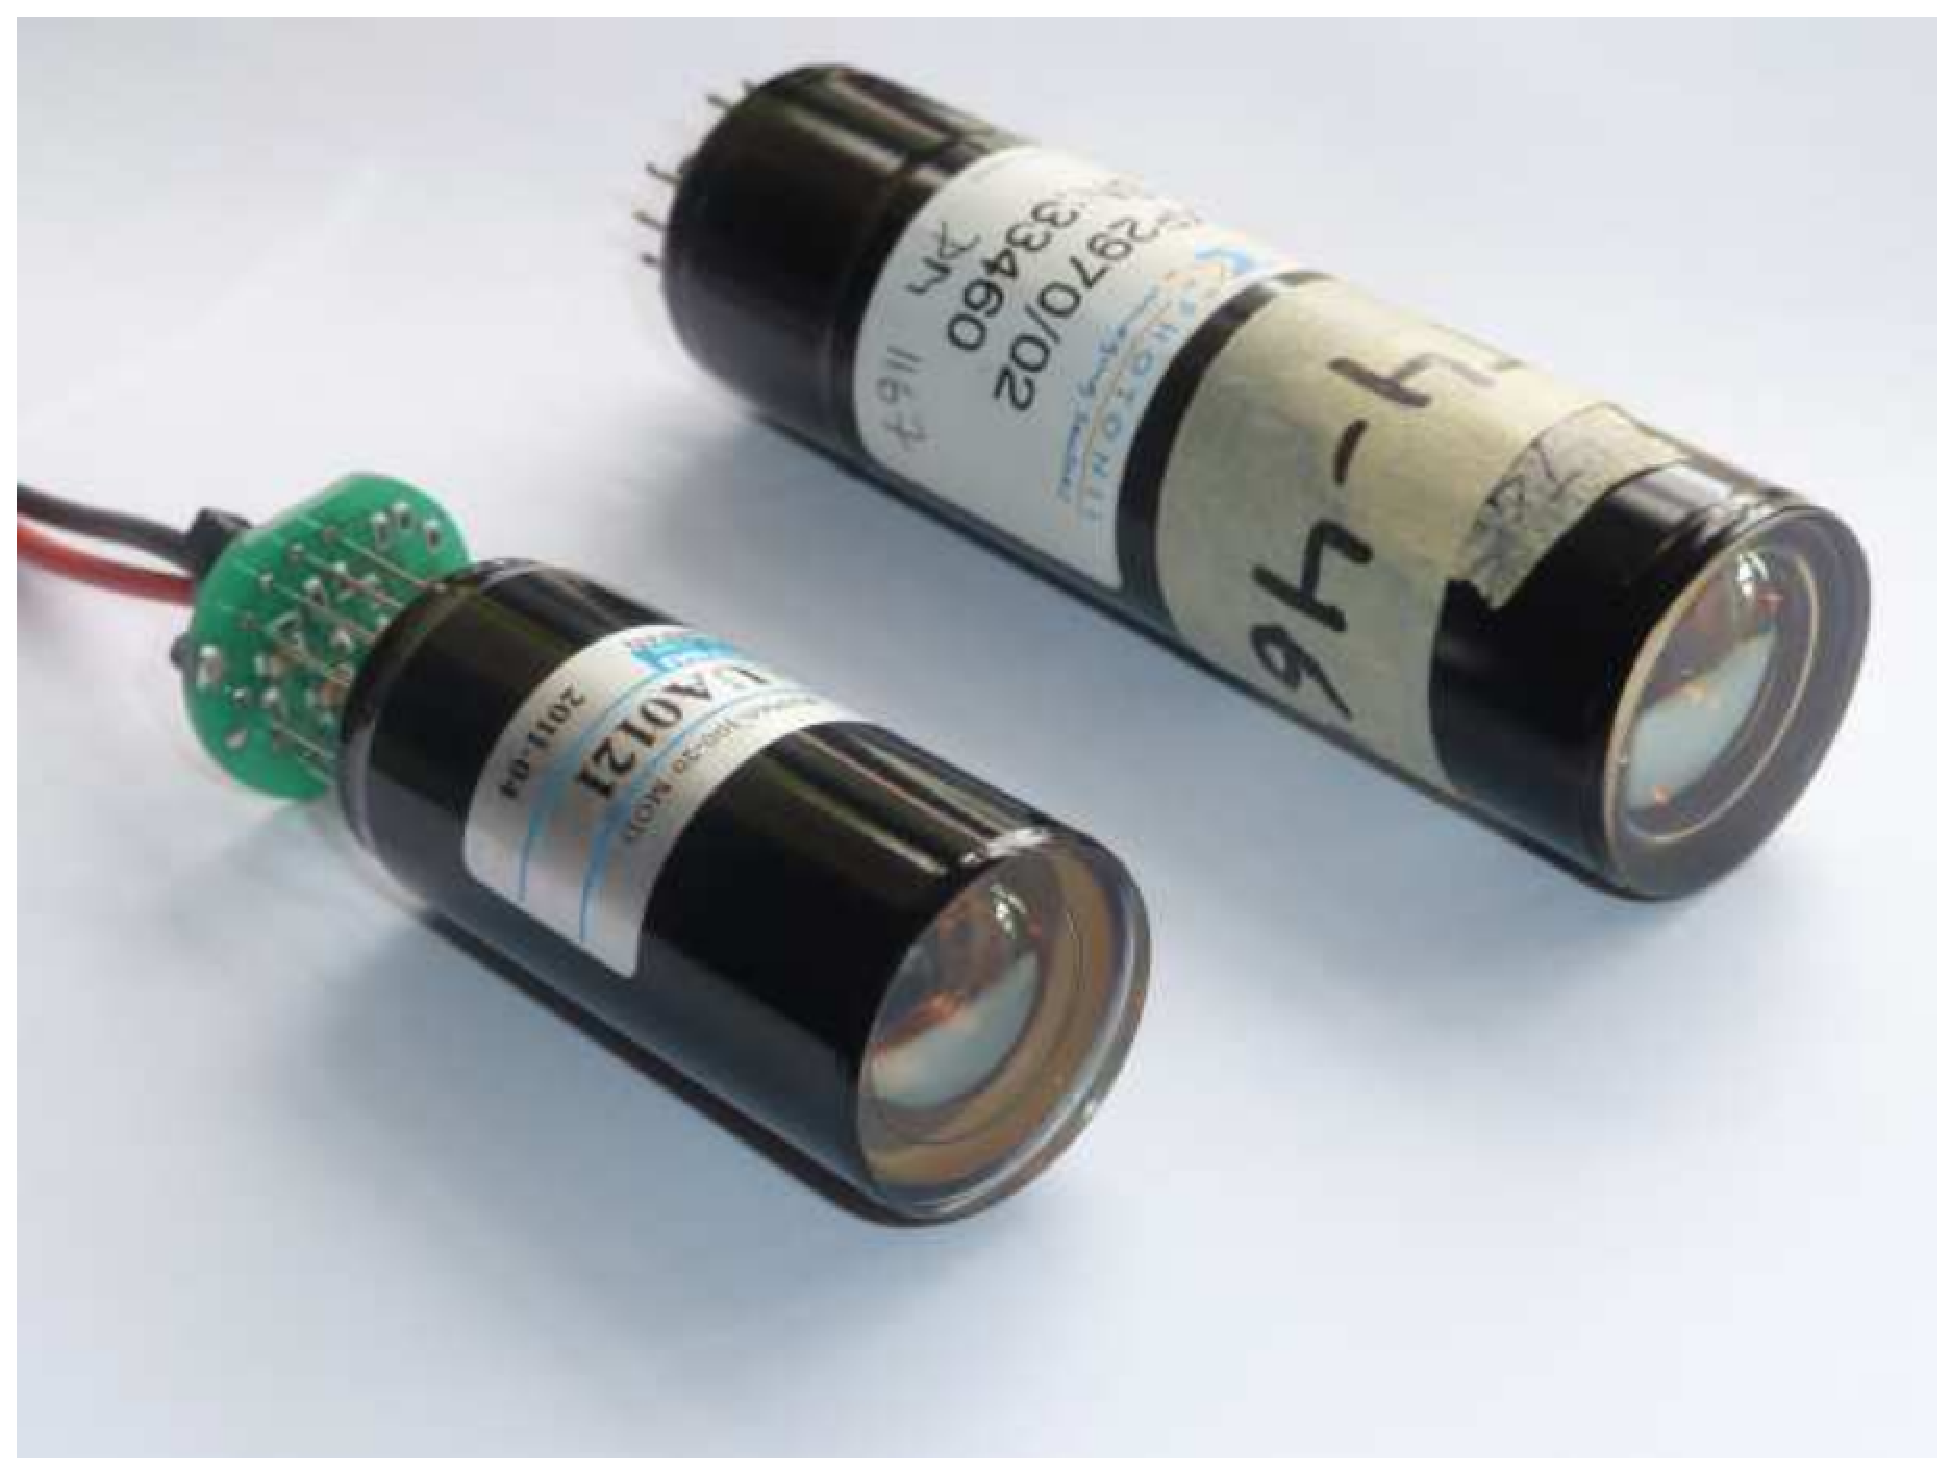
\includegraphics[width=0.75\textwidth]{images/pmt_models}
    \caption[PMT Models]{The two PMT models used in the VERITAS cameras. \cite{pmtmodels}}\label{fig:pmtmodels}
  \end{center}
\end{figure}

The PMTs' output signals are first sent through an amplifier, before travelling down a \nicetilde45m (cite??) cable to electronics stationed near the telescope.
The electronics then digitize the signal.

The first circuit that the signal passes through is a Constant Fraction Descriminator (CFD) circuit.
This circuit duplicates the signal voltage pulse from the PMTs, inverts and delays the duplicate pulse, and adds it back to the original pulse.
This combined pulse then crosses the zero-volts threshold (called a Zero Threshold Descriminator) at the same time (how 'same'?? within 1 ns??) as the original pulse reaches its peak, acting as a maximum-voltage detection circuit.
When a maximum voltage is detected by the circuit, it emits a 10ns trigger pulse to other electronics.

The use of this circuit has two main benefits.
The first use is that the CFD circuit will trigger at the same time regardless of the pulse size (??).
If a simple threshold trigger is used to detect a signal pulse, the time of the trigger will be earlier for larger pulses, and later for smaller pulses.
The CFD's zero threshold trigger time is around the time when the signal voltage pulse is at 75\% of its maximum value. (cite??)

The second use is that when the CFD circuit detects a voltage pulse larger than a given maximum threshold, it can emit an extra logic trigger, called a low-gain trigger.
This extra low-gain trigger can then be used by later electronics to determine the rough size of the original signal voltage pulse.

CFD behavior cite??

CFD model??

FADC model??

After the CFD emits a trigger pulse, the signal voltage pulse is passed to another circuit for digization, a Flash Analog-to-Digital Circuit, or FADC.
This FADC circuit then, for each nanosecond time bin, measures how large the voltage pulse is with a series of 255 (??) constant-voltage thresholds.
The highest threshold that is crossed in a single time bin then determines the digital voltage value that is saved to the FADC buffer for that time bin.

If the low-gain trigger pulse was also recieved by the FADC, then the signal voltage pulse is de-amplified before being digitized, since the CFD low-gain threshold is set to lower than the FADC maximum digitizable voltage.
If this low-gain triggering did not take place, then the FADC would become saturated, which effectivly hides how large the voltage pulse actually is.
Once the voltage pulse is digitized, it is saved to a rolling buffer (how long is the buffer??) in the FADC, waiting for other future triggers to occur.

\subsection{PMT Upgrade}
In summer of 2012, all PMTs in the telescopes were replaced with improved PMTs.
Specifically, the original Photonis XP2970 models were replaced with the Hamamatsu R10560-100-20 MOD.
This was done because that R10560 has a considerably higher quantum efficiency (\nicetilde$90\%$), compared to the XP2970 (\nicetilde$75\%$).
This higher quantum efficiency means more photons from a shower are detected by the PMT, which means VERITAS is more sensitive to lower energy gamma rays\cite{pmtmodels}.
In addition, the voltage pulse due to a single photoelectron is thinner with the R10560 compared to the XP2970, as shown in figure \ref{fig:pmt_pulse_widths}.

\begin{figure}[h]
  \begin{center}
    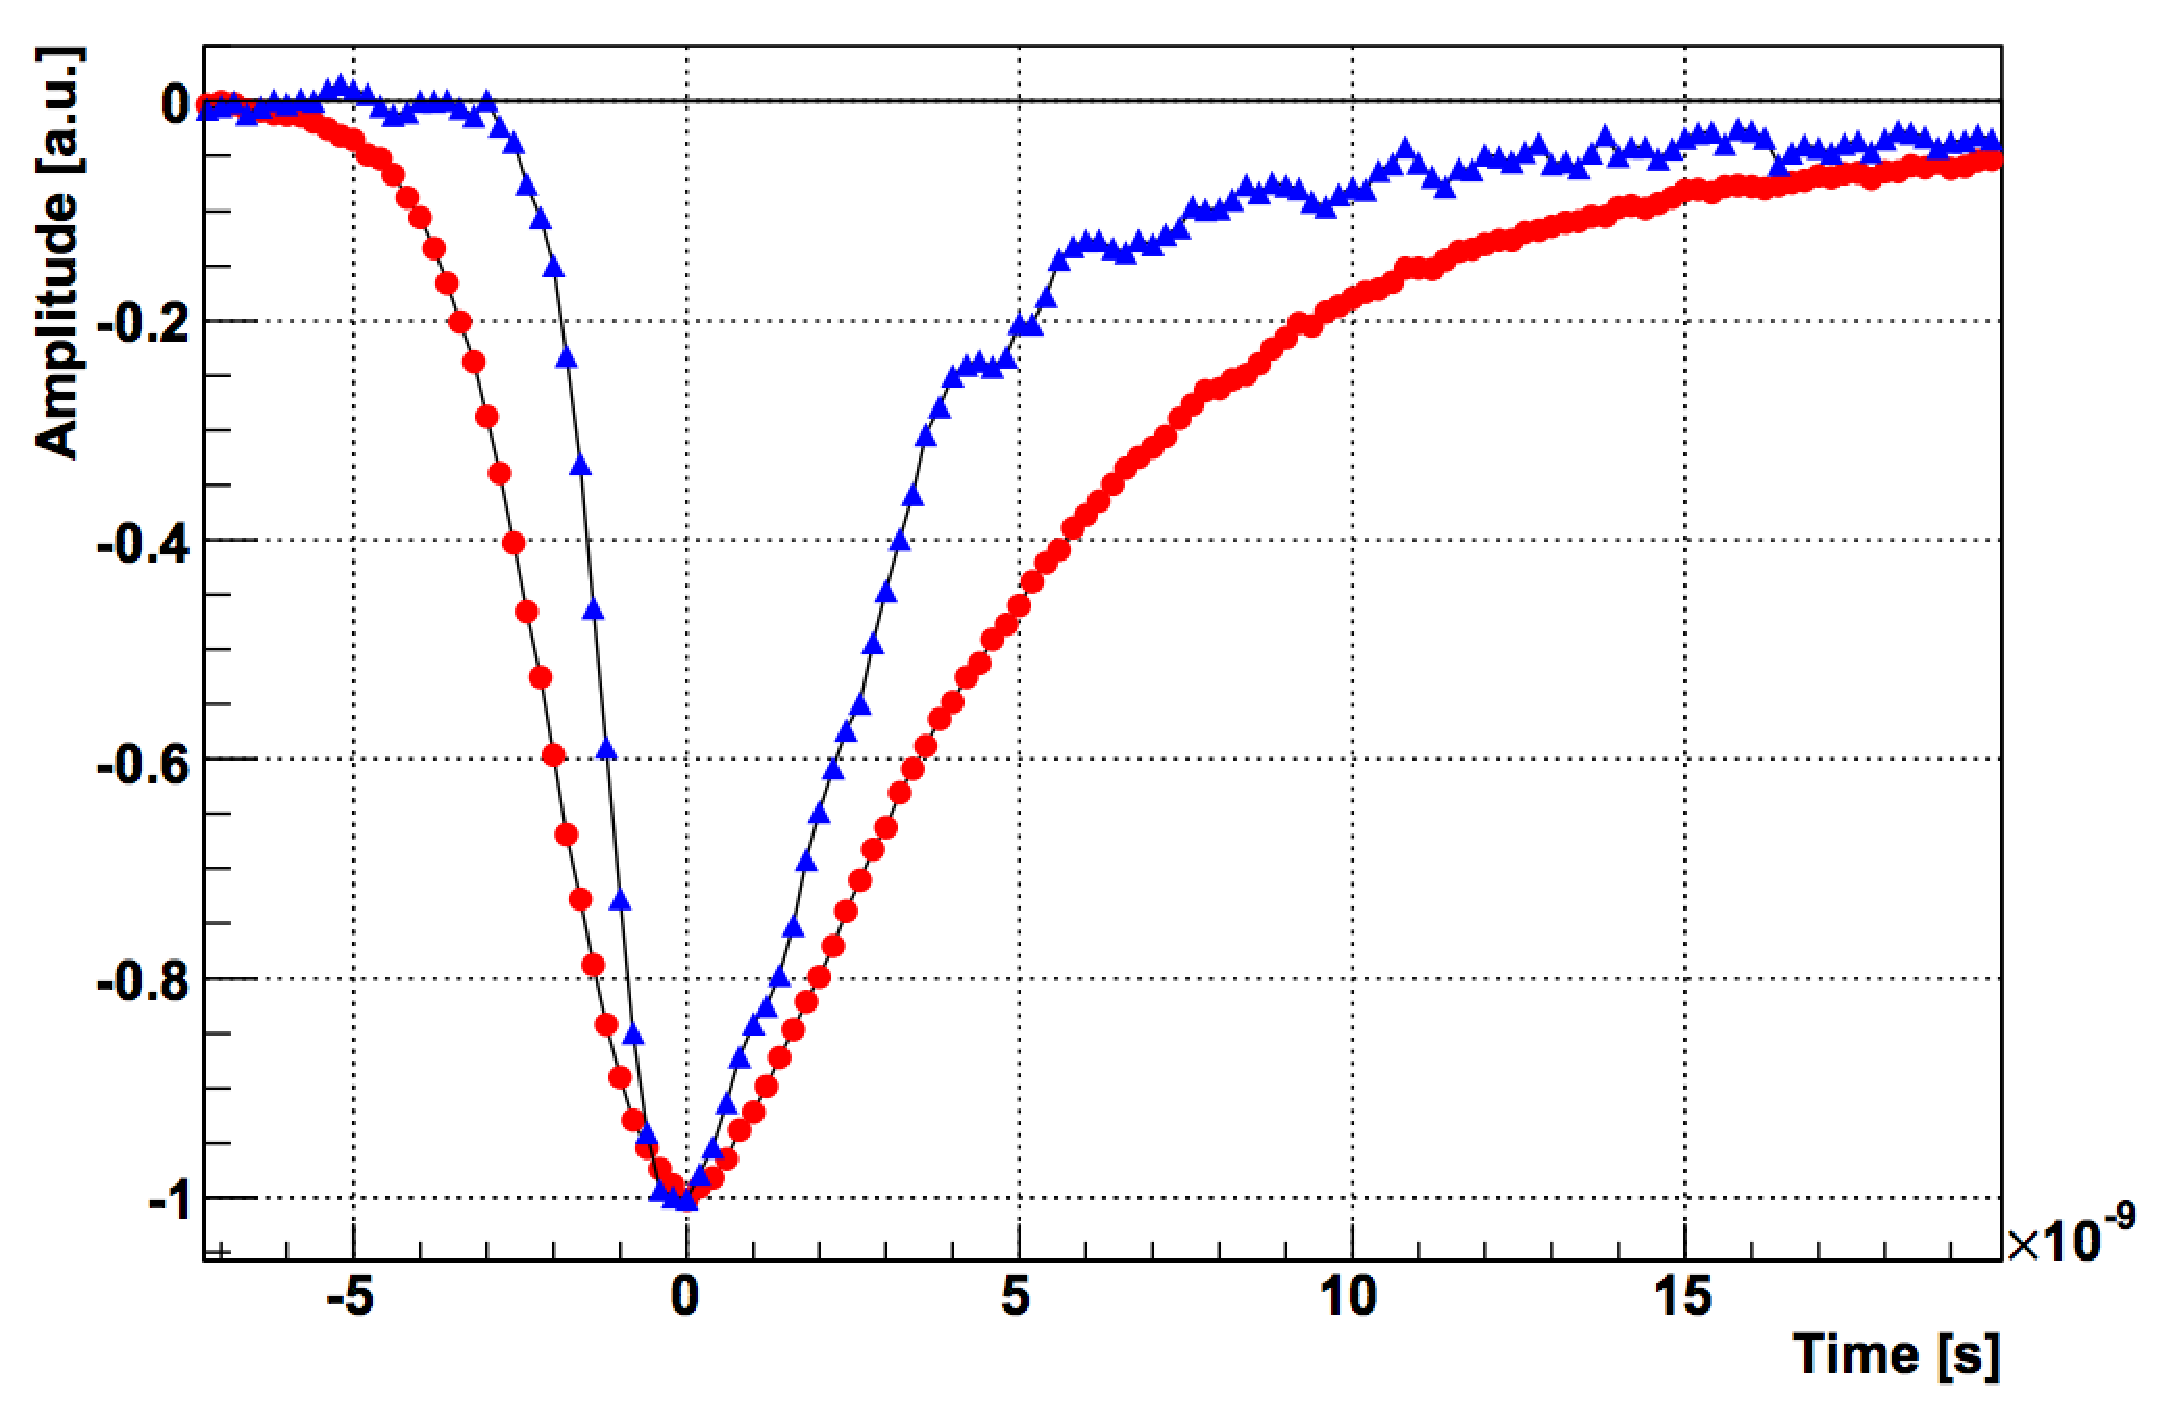
\includegraphics[width=0.75\textwidth]{images/pmt_models_pulsewidths.eps}
    \caption[Pulse Widths]{Pulse widths of the old XP2970 (red circles) and the new R10560 (blue triangles), taken from \cite{pmtmodels}.  Plots are the average of many afterpulses, normalized to the maximum amplitude.  Pulses shown include dispersion due to a \nicetilde55m coaxial cable between the PMTs and the digitizer boards.}\label{fig:pmt_pulse_widths}
  \end{center}
\end{figure}

The data used in this thesis was taken both before and the upgrade, which means the telescope performance is different for these two time periods.
This is accounted for by separate simulations for each PMT model, mostly resulting in different effective areas at the lower energies.


\subsection{PMT Calibration}

While the VERITAS PMTs are all the same model, there are still differences from PMT to PMT that can impact any data taken, and.
Primarily, these differences can cause the same number of incident photons to create differently-shaped output voltage pulses in each PMT.
To account for these differences, there are several calibration procedures that are applied nightly or semi-nightly.
These are performed with a set of flashing LEDs, placed on the camera such that their light bounches off the mirrors and back onto the PMTs.

In the first procedure, the LEDs are flashed at ~10hz at the beginning of each night.
While the LEDs are flashing, the average pulse width from each PMT is monitored.
Then, the High Voltage is adjusted for each group of PMTs to make their pulse widths as similar as possible (there are several PMTs connected to each high voltage crate).
This must be done nightly, because just like each PMT is unique, each PMT's temperature dependence is also unique.

In the second procedure, once every several nights the single-photoelectron curves for each PMT are measured.
This is done by placing an opaque (~mm-thick metal) plate over the PMTs, with a single 3.1mm hole drilled over the location of each PMT.
The LEDs are then flashed repeatedly.
As the opaque plate has holes for each PMT, each PMT gets on average 0-5 photons per flash.
Large numbers of flashes can then be used to build statistics on each PMTs' distribution of pulse widths.
By examining a histogram of these pulse widths, one can see poison-statistics peaks (from the PMT's quantum efficience) that are formed for the 1, 2, 3, and further integer numbers of photons.
And then ?? is done with this information?

These calibration techniques are further detailed in \cite{calib_techniques}.


\section{Trigger System}\label{sec:trig}

The operation of VERITAS requires digitizing voltage pulses roughly once per nanosecond, per photomultiplier tube.
This means that, with 255 voltage levels, 1 second of raw voltage data would require 2 Terabytes of space.
As this is unfeasable with today's computing systems, only subsets of the raw pixel voltages are saved when certain triggers are met.
To complicate matters, photons from atmospheric muons and the night sky background can also cause voltage pulses similar to a gamma ray shower.
Thus, VERITAS has a system of triggers that reduces the amount of raw data that is saved, while also partially filtering out non-gamma-ray events.

The L1 is the first and lowest level trigger.
An L1 trigger (sometimes called a pixel trigger) is emitted when a PMT's CFD circuit detects a signal voltage above a given threshold, typically in the 10s of mV.
This threshold voltage is varied throughout datataking by a rate-feedback system (elaborate more??).
The L1 trigger is emitted at the point in time when the voltage pulse is approximatly 75\% of its maximum (??).
Once emitted, the L1 trigger is sent to a per-telescope FPGA (see https://arxiv.org/pdf/1307.8360v1.pdf ??) circuit board for the next level trigger.

The FPGA's L2 trigger, or image trigger, is emitted by the FPGA when a group of L1 triggers meet certain conditions.
These conditions include that multiple L1 triggers fall within a certain time window, and that multiple L1 triggers come from one of several predefined shapes, or templates.
The coincident time window varies. (elaborate??)
There are several patterns. (elaborate??)
The pattern requirements help reduce the number of triggers from non-gamma-ray sources.
Night sky background photons are only able to trigger individual pixels, and muons tend to create ring-shaped images.
Once one of these patterns occurs in a time window, the FPGA emits an L2 trigger, which is sent to the array trigger system.

The array trigger system, or L3, is a computer (box?? circuit??), which looks for coincident L2 triggers that fall within a \nicetilde50ns time window.
Why 50ns??
This window is also varied for each telescope based on the azimuth and elevation of the pointing, as these can introduce nanosecond delays between images.
During a typical observation period, the L3 trigger rate is around 200-300Hz.

Once an L3 trigger is invoked, a signal is sent to all telescopes (all or just L2-triggered telescopes??) that the digitized voltages for all pixels in the cameras should be read out from their buffers, and saved to memory.
These pixel voltages are then processed by the analysis software to reconstruct the gamma ray events.



\subsection{Deadtime}
When the L3 trigger is invoked and the buffers are being read out, the electronics are unable to store new PMT voltages in the buffers.
Being unable to store new PMT voltages effectivly reduces the amount of time spent observing gamma rays.
This lost time is usually referred to as deadtime.
As the deadtime is a fixed (is it fixed??) time loss per event, the percent of time lost due to event readout rises with the a higher frequency of readouts.
This means that at an L3 trigger rate of \nicetilde300Hz, approximately \nicetilde12\% of the time is lost due to buffer readouts.

Since the L3 rate varies over the course of a run, this means that the deadtime also varies.
This is accounted for in the flux calculation in section ??.

\subsection{Time Pedestal Calibration}
As all PMTs and signal cables are not identical, there are differences in how long a voltage pulse takes to travel.
More specifically, the time between a) when the photon strikes the PMT cathode ?? and b) when the voltage pulse sets off its L1 trigger, can vary from pixel to pixel.
This is usually measured by looking at the average arrival time of many events over all camera pixels.
By looking at the average arrival time, pixels that are consistanly early or late can be accounted for, which improves image identification.

\section{Epochs}\label{sec:epochs}
After being built, VERITAS has evolved over several years, with collaboration members upgrading it to improve performance.
However, these major differences need to be taken into account in the analysis chain.
To organize these differences, in the data they are referred to as epochs 1, 2, 3, 4, 5, and 6 (usually denoted as V1, V2, V3, V4, V5, and V6).

As the first three telescopes were constructed and brought online, data taken after each is the first, second, and third epochs.
Telescope 1 was placed at (-37.6, -23.7), telescope 2 at (44.1, -47.7), and telescope 3 at (29.4,60.1), where the coordinate system's origin is at 31.675N, 110.962W??, the X axis points East, and the Y axis points North, and both axes are in meters(??).
In 2007, the fourth telescope was finished at (-35.9,11.3), and data taken between this point in time and the next major upgrade is considered the fourth epoch.

In September 2009, telescope 1 was moved to a new position (135.4,-8.61), after it was demonstrated with simulations that it would grant a \nicetilde30\% improvement in sensitivity \cite{veritas_t1_move}.
Data taken after this relocation is referred to as the fifth epoch.

In August 2012, the PMTs in all cameras were replaced with improved PMTs that had a higher quantum efficiency, improving the telescopes ability to resolve images\cite{pmtmodels}.
Data taken after this upgrade is considered part of the sixth epoch.

As these different epochs have different telescope configurations, the instrument response functions are different, meaning each epoch behaves in a quantifiably distinct manner.
For the Dark Matter analysis described in this thesis, only data from the fifth and sixth epochs are used.



\cleartooddpage[\thispagestyle{empty}]
\chapter{Gamma Ray Reconstruction}\label{ch:grrecon}

In chapter \ref{chapter:veritas}, it was explained how the trigger system preserves PMT voltage traces of potential events.
To reconstruct gamma rays, the voltage traces caused by cherenkov photons must be identified and combined to form an image of the original cherenkov shower.
Then the shower images from multiple telescopes can be used to reconstruct the original gamma ray's energy and direction.

\section{Pedestal Variation}
  Before reconstructing any events, the pedestal and pedestal variations (pedvars) must be calculated.
  These are done by artificially triggering all pixels once per second during observations, in order to record events that contain only noise.
  The average of the digital counts (dc) of all noise-events for each pixel is then the pedestal.
  From this pedestal, the pedvars are then calculated as the rms of the all the dc counts in all noise-events, which can be visualized as the distribution of dc around the mean dc.

\section{Pixel Identification}
  The first step is to determine which pixels are part of a shower image.
  This is done by subtracting the digital counts pedestal from the entire trace, and then integrating the total dc in each voltage trace.

  The start of a potential voltage pulse is the time when the voltage trace is at half of its maximum value, called $T_{0}$.
  Around time $T_{0}$, the trace is integrated a second time with a smaller time window (usually either 14 or 24 ns wide, at $T_0$ - 30\% of the window size), to reduce the inclusion of dc from sources of noise (NSB and electronics).
  This two-pass algorithm is usually referred to as the double-pass method\cite{doublepass}.
  If a pixel's second-pass total dc is higher than 5 times the pedvar, then it is considered an image pixel.
  If it is between 2.5 and 5 times the pedvar, it is considered a border pixel.

  Once all pixels have been classified, isolated border pixels that have no neighboring image pixel are removed from the image, as they are more likely to be due to noise than cherenkov photons.
  Then, the time gradient from the image and border pixels can be found by performing a linear fit of the $T_{0}$ times.
  This time gradient can then be used to place a (more accurate) third integration window with 30\% of the window before each pixel's $T_{0}$, to more accurately measure the charge due to cherenkov photons in the pixel.

  From the image pixels, border pixels, and time gradient, the shower's Hillas parameters \cite{hillas_params} can be calculated.
  These include the size of the shower in photoelectrons (or equivalent units), the shower center of charge, angle, length and width.
  The center of charge is the charge-weighted average of all image and border pixel positions.
  The angle of the shower determines how the image's major axis is oriented in the camera.
  The shower length and width are determined by the rms of the shower image along its major and minor axes, respectively.

\section{Position Reconstruction}\label{subsec:posrecon}
  By examining the images from multiple telescopes, the initial position of the event can be determined.
  This is done by overlapping all telescope images in a single camera coordinate system, and projecting each image's major axis backwards in time.
  These drawn lines should intersect very close together, and the average of the intersection points determines the event's initial direction.

  In averaging the intersection points, weighting for each intersection can be applied based on the angle between the two lines.
  This improves the reconstruction, because the intersection point from two images at \ang{90} angles will be less sensitive to image fluctuations than two images at \ang{160}, as shown in Figure \ref{fig:largeintersectangle}.
  Additionally, the disp method described in section \ref{subsec:disp} can be utilized to offer improvements at lower telescope elevations.

  \begin{figure}[ht]
    \centering
    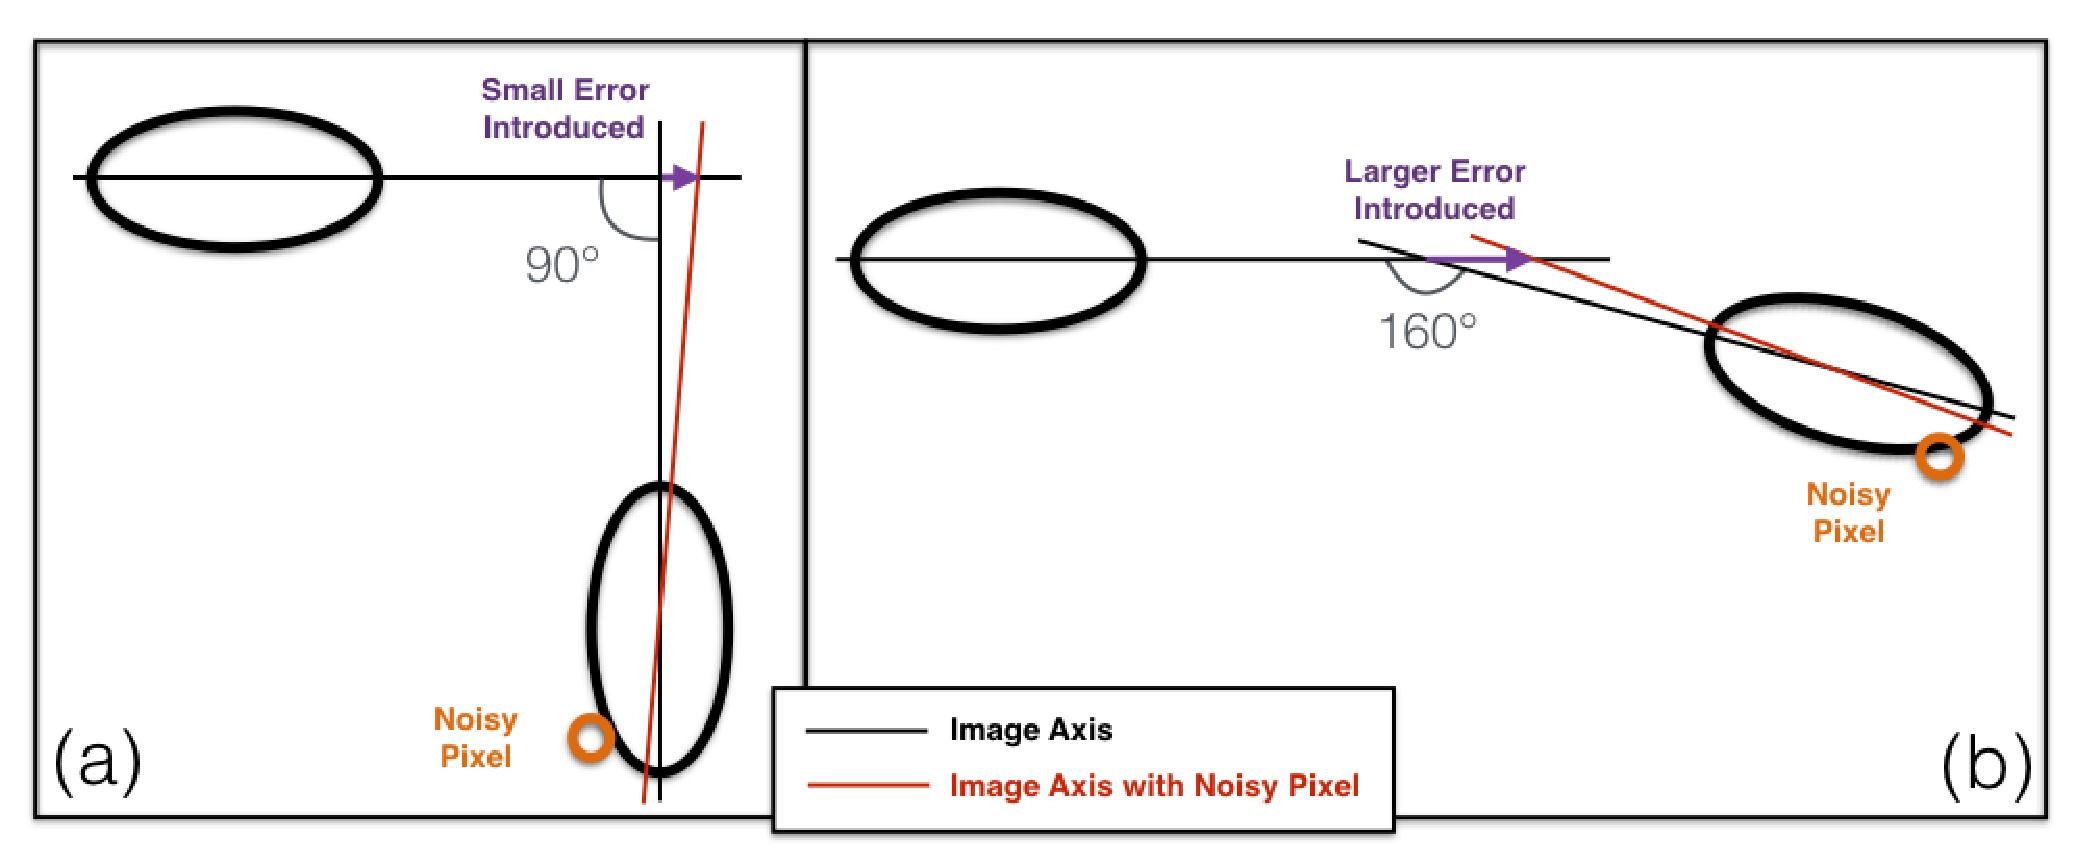
\includegraphics[width=0.95\textwidth]{images/large_angle_image_intersection_error_cropped.eps}
    \caption[Large Image Intersection Angles]{
      In diagram (a), when a noisy pixel is added to an image, the reconstructed position is only moved a small distance (the purple arrow).
      In diagram (b), due to the large angle between images, the error in the reconstructed position is much larger.
    }
    \label{fig:largeintersectangle}
  \end{figure}

  \subsection{Angular Reconstruction Neural Network}\label{subsec:disp}
    At high elevations, shower images often form small intesection angles, because the telescopes are spread out in two dimensions, relative to the shower in the atmosphere.
    At low elevations near the galactic center, however, the telescope array flattens into one dimension, which makes the shower's impact parameter (the shortest distance between the telescope and the shower core axis) smaller for two of the telescopes.
    These two closer telescopes then have very short, almost circular images, which increases the sensitivity of those two image axes to noisy pixels or shower fluctuations, as shown in Figure \ref{fig:showerhighlowelev}.
    This also causes the remaining telescope images to have large intersection angles, which also reduces the accuracy of the position reconstruction.

    \begin{figure}[ht]
      \centering
      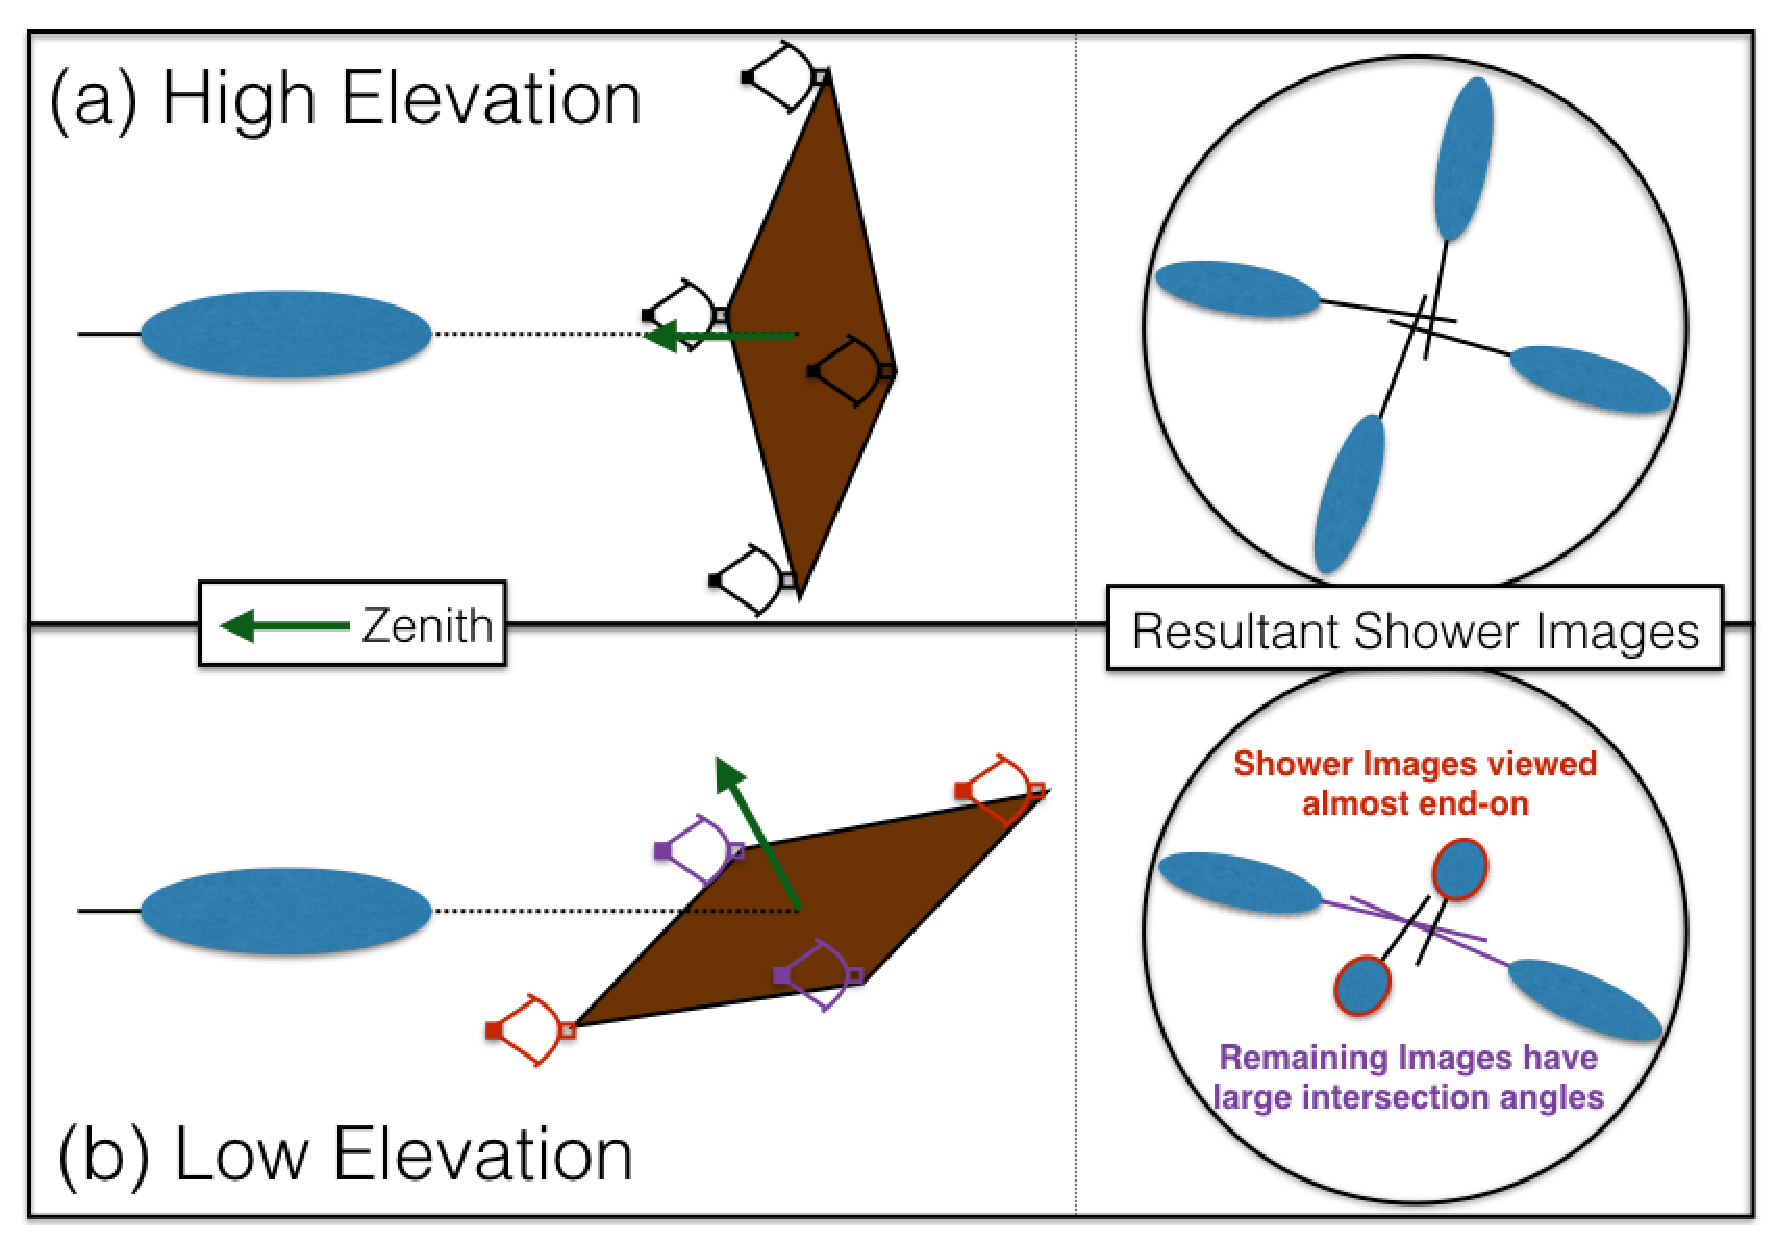
\includegraphics[width=0.75\textwidth]{images/high_elevation_vs_low_shower_images_cropped.eps}
      \caption[Shower Images at High and Low Elevations]{
        In Figure (a), high elevation showers produce long images in all four telescopes.
        In Figure (b), lower elevation showers produce shortened images in two telescopes, and the remaining images form large angle intersection.
      }
      \label{fig:showerhighlowelev}
    \end{figure}

    To better handle these near-parallel image axes at low elevations, the reconstructed position can be determined from more parameters than just the weighted image axes intersection points.
    From simulations, the distance between the center of the Hillas shower image and the true position can be calculated, where the angular distance between the two is the \disp{} parameter\cite{Senturk:2011}, shown in Figure \ref{fig:dispdiagram}.
    Then, this \disp{} parameter can be provided to a machine learning algorithm \cite{Beilicke2012NIM}, along with other image parameters like:
    \begin{description}
      \item[\textit{width}:] image angular width
      \item[\textit{length}:] image angular length
      \item[\textit{wol}:] $\frac{\textrm{width}}{\textrm{length}}$
      \item[\textit{size}:] total image dc
      \item[\textit{ntubes}:] number of pixels in the image
      \item[\textit{loss}:] fraction of image pixels at the edge of the camera
      \item[\textit{asym}:] distance between image center-of-dc and the pixel with the highest dc
      \item[\textit{tgrad}:] the slope of the linear time fit to the pixel arrival times
      \item[\textit{cross}:] angular distance between the image center and the reconstructed gamma-ray position
    \end{description}
  % list of training parameters: grep "AddVariable" $EVNDISPSYS/src/trainTMVAforAngularReconstruction.cpp
  % how variables are calculated: grep -P "fParGeo.+\=" $EVNDISPSYS/src/VImageParameterCalculation.cpp
  % asym: http://inspirehep.net/record/1395717/files/RdelosReyes.pdf
  % Once trained on these parameters, the machine learning algorithm can construct a boosted decision tree for determining any new image's \textit{disp}, which can then be used with the image axes intersections to improve the gamma-ray reconstructed positions.


    \begin{figure}[ht]
      \centering
      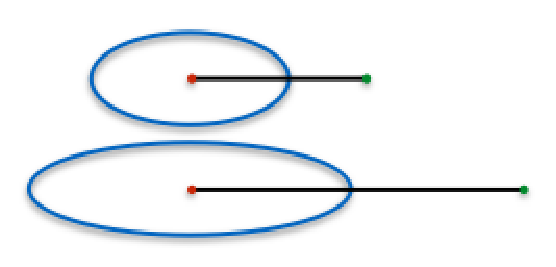
\includegraphics[width=0.5\textwidth]{images/disp_parameter_cropped.eps}
      \caption[Angular Reconstruction Disp]{
        The \disp{} parameter is the angular distance between the center (red dot) of a hillas image (blue oval) and the true sky position (green dot).
        Generally, longer shower images have a larger \disp{} angle.
      }
      \label{fig:dispdiagram}
    \end{figure}

    % https://veritas.sao.arizona.edu/wiki/index.php/BDT_Angular_reconstruction
    These parameters for thousands of simulated showers can then be used to train a boosted decision tree forest (BDT) that estimates the most probable \disp{} for a new shower's images.
    This most-probable \disp{} can then be used with the image axes intersection points to more accurately reconstruct the original gamma-ray point of origin.
    
    Once the training is complete, it is tested on a separate set of 17,000 simulated events, which are plotted in Figure \ref{fig:disptraining}.
    The x axis describes the true \disp{} value for each event, while the y axis describes the \disp{} value estimated by the BDT, with a black $x=y$ line marked, which represents a perfect 1:1 \disp{} reconstruction.
    As events fall on the $x=y$ line, it can be concluded that the BDTs are able to predict the correct \disp{} value for most images.

    % made from screenshot of last slide in Dropbox/Presentations/20160719_Group_Meeting.key
    \begin{figure}[ht]
      \centering
      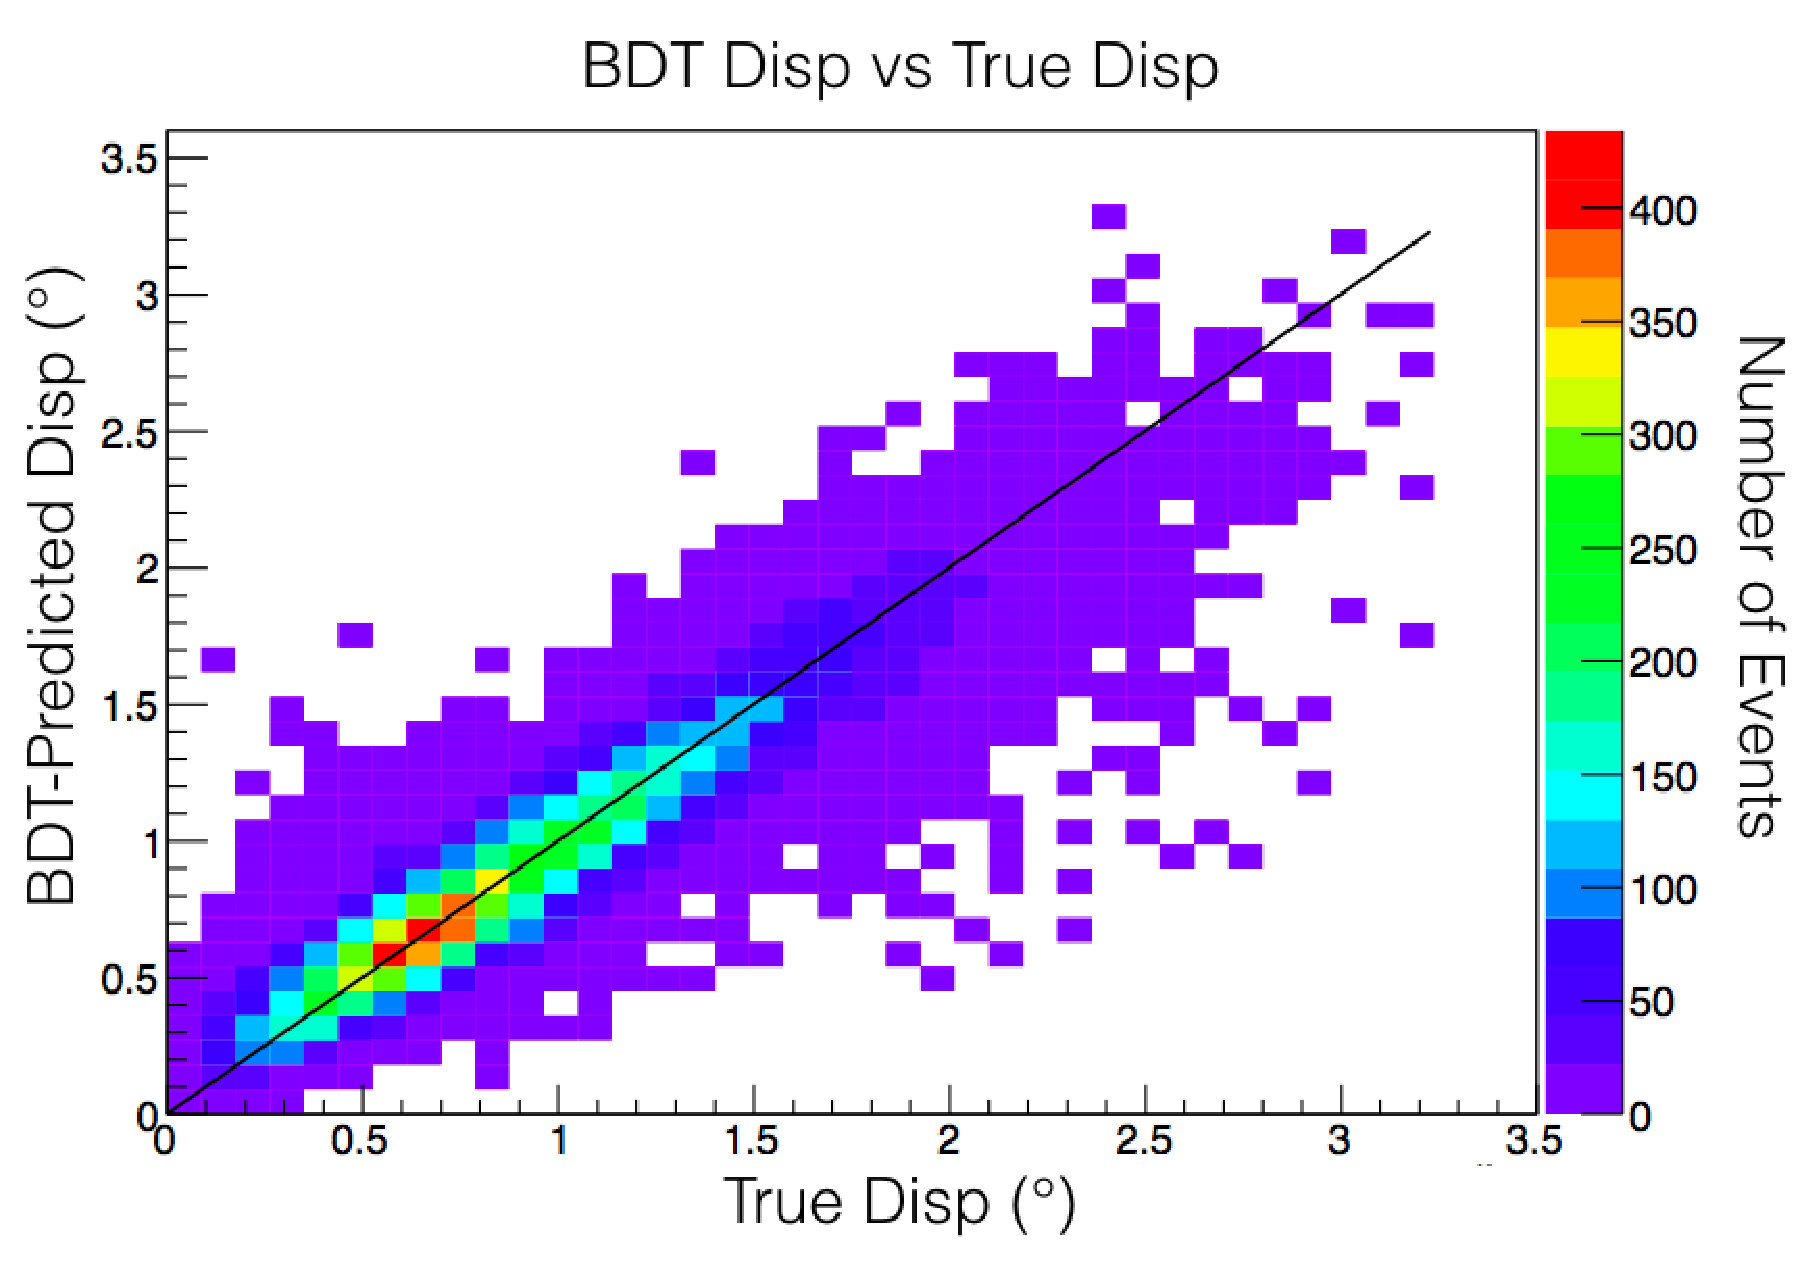
\includegraphics[width=0.85\textwidth]{images/disp_training.eps}
      \caption[Disp BDT Training]{
        The true \disp{} vs the BDT-predicted \disp{}, for \nicetilde17,000 gamma-ray event images in T1, from 500\GeV to 200\TeV.
      }
      \label{fig:disptraining}
    \end{figure}

    The small improvement in the position reconstruction due to the \disp{} method can be seen in Figure \ref{fig:disp_event_offset}.
    With the Geometric (red) events, more are concentrated further from the point source, while with the Disp method, somewhat more are concentrated at the source itself.

    \begin{figure}[ht]
      \centering
      \includegraphics[width=0.85\textwidth]{images/disp_event_offset_hists/dispgeom_comparision.eps}
      \caption[DISP Offset Improvement]{
        The number of events per solid angle at different angular offsets from the Crab and the Galactic Center, with both Geometric and Disp reconstruction methods.
        (Would be great to put the mean and RMS on the plots, so you can quantify the differences. --Orel??)
        (still needs fixing??  Why does the crab see so little benefit??  why does the disp mean move left in the crab, but right in Sgr A*?)
      }
      \label{fig:disp_event_offset}
    \end{figure}

\section{Energy Reconstruction}\label{subsec:enrecon}
  To reconstruct the energy of each shower, a database of simulated showers is built.
  This database includes the width and length of the shower, how far away its core position is, how bright it was, as well as its reconstructed and true energy.
  By scanning through this database for showers that are similar to the one being constructed, the most similar-looking shower then indicates the true energy(is there any interpolation?? -Orel, ask gernot).

\section{FITS Conversion for Gammalib and CTOOLs}
  Once gamma rays have been reconstructed with event display, they must be converted to a FITS file format compatible with Gammalib and CTOOLS.
  This format consists of a FITS file with an event list table, containing each gamma ray, its energy, sky direction, and time.
  This also includes meta information about the event list like the telescope's pointing target and the start and end times of the event list.
  This FITS file can then be read into Gammalib and CTOOLS \cite{gammalibctools}.

  In addition to the event list, the instrument response functions (IRFs) must also be imported into Gammalib and CTOOLS.
  These IRFs consist of the effective areas, the point spread functions, the background models, and the energy dispersion.
  The effective area quantifies the total gamma-ray collection area of the observatory, needed for spectral measurements, and is described in subsection \ref{subsec:effarea}.
  The point spread function quantifies the distribution of true positions for a reconstructed position, needed for identifying point sources and extended spatial structures, and is described in subsection \ref{subsec:psf}.
  The background models measure the relative number of observed events in different parts of the camera, and their construction is described in subsection \ref{background_production}.
  The energy dispersion quantifies the distribution of true energies for a given reconstructed energy, and is discussed in subsection \ref{subsec:edisp}.

  Each of these IRFs vary in a parameter space with several dimensions, including event Energy, reconstructed distance from the camera center, telescope elevation and azimuth, night sky background noise, and the atmospheric density.
  In CTOOLS' default configuration, all IRFs are stored in a single directory of files, and each event list contains a filepath reference to indicate which volume of the parameter space it uses.
  Once each volume is loaded, individual events can then interpolate their specific effective area, psf, and energy dispersion (the backgrounds are utilized differently, as discussed in subsection \ref{background_production}).

  However, the galactic center is at an elevation of \ang{30}, much lower than most VERITAS observation targets.
  At this elevation, with its field of view of \ang{3.5}, the airmass column density ($g/cm^{2}$) is 20\% higher at the bottom of the camera than at the top.
  Add to this that during a single 30 minute observation, the elevation of the Galactic Center can change by several degrees, means the airmass in view of the camera may change rapidly, meaning the IRFs may become time dependent.

  To allow for the inclusion of this time dependence in the analysis, an alternate way of storing the IRFs was chosen, diagrammed in Figure \ref{fig:fits_scheme}.
  First, one observation (typically 20-30 minutes long) is broken up into \nicetilde8 minute chunks.
  Each chunk is then converted to an event list, and saved to a FITS file.
  In addition, the needed effective areas, psfs, and background models are also written to the same FITS file.
  As each event list covers a small region in time, the IRF tables only need to contain the dimensions of the parameter space that can change during one chunk, such as event energy and distance from camera center.

  \begin{figure}[ht]
    \centering
    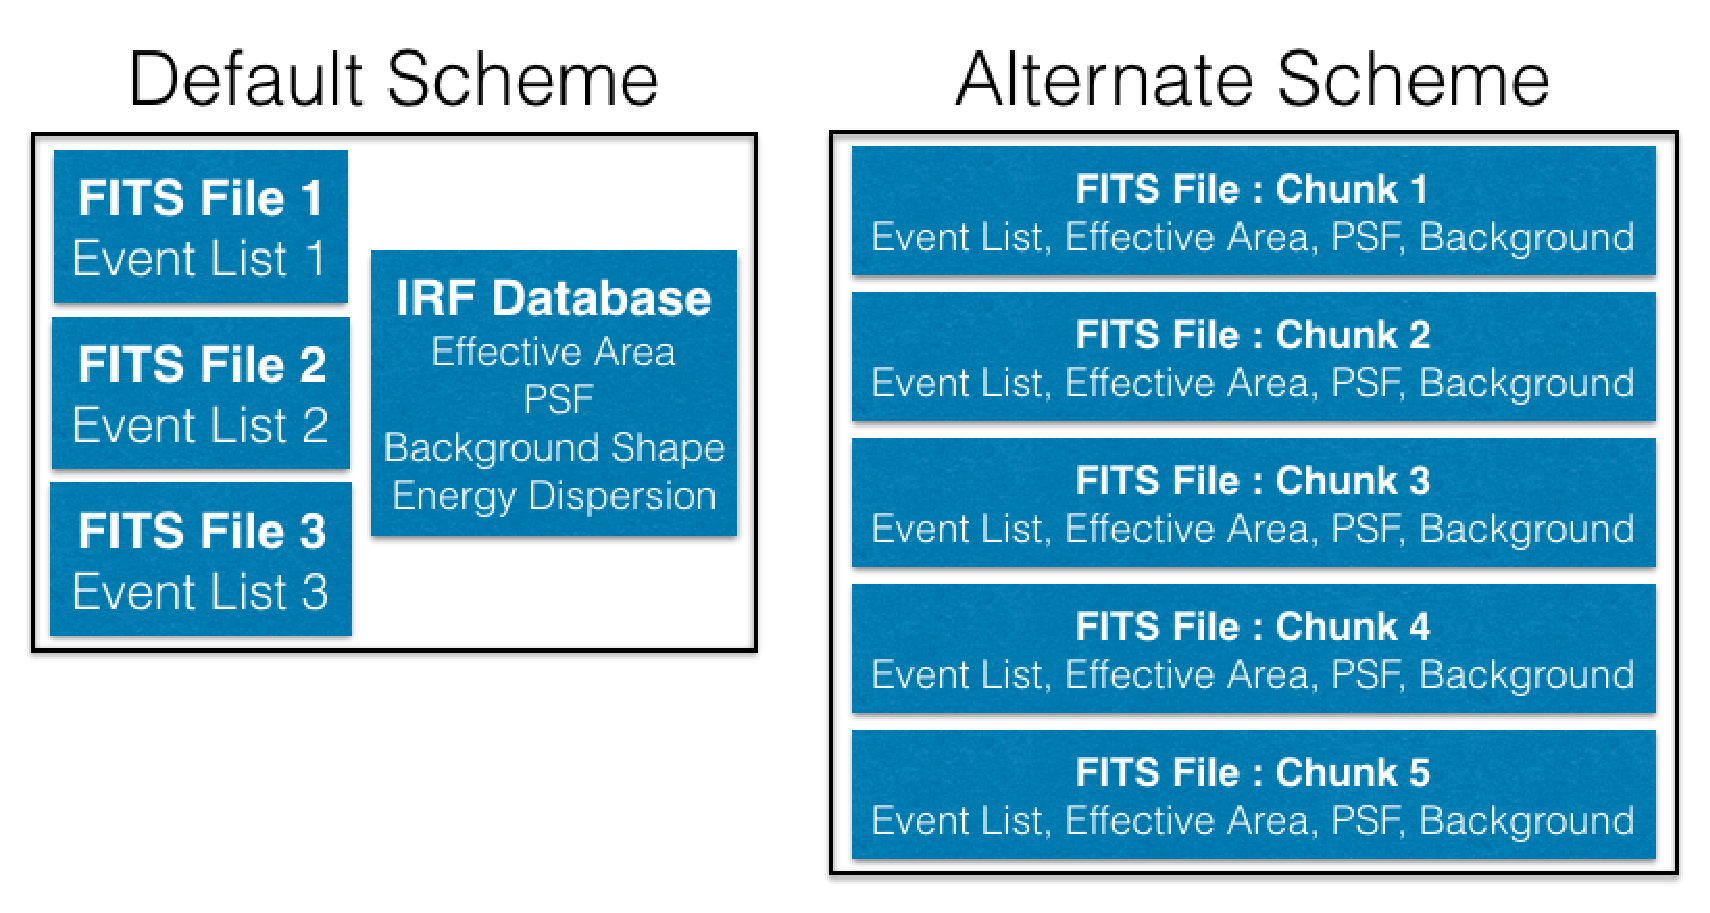
\includegraphics[width=0.75\textwidth]{images/FITS_diagrams_alternate_scheme.eps}
    \caption[FITS File Event Storage Schemes]
    {Fits file storage schema.}
    \label{fig:fits_scheme}
  \end{figure}

  The end result is that a 30 minute observation can be broken into several FITS files (called chunks), where each chunk file is independent of any outside references, contains all needed IRF information, and only takes up \nicetilde\SI{5}{MB} on disk.
  This makes it ideal for an analysis program to automatically download any needed data over an internet connection, as each chunk is tiny and has no outside dependencies.
  As gammalib and CTOOLS expect the default FITS file scheme, a python function was written to automatically load all event and IRF tables from a single fits file, and import this information into gammalib's GObservation class.

  There were minor issues with converting the IRFs that are noted in the following sections.


  \subsection{Effective Area}\label{subsec:effarea}
    % use effective area as a casual noun!
    % plot of effective area vs energy
    Effective area is the measure of how large an observatory's collection area is, determining how many gamma rays can be detected per unit time, solid angle, and energy.

    For each point in the parameter space, the effective areas are calculated with many Monte Carlo gamma ray simulations.
    This is done in the shower plane, the plane perpendicular to the line drawn between an observing source, and the center of the observatory.
    The effective area is then calculated via:
    $A=\pi R^2 \frac{N_{\text{survived}}}{N_{\text{simulated}}}$
    where R is the radius of the area within which simulated showers are directed to fall, $N_{\text{simulated}}$ is the number of showers that were initially simulated into the area, and $N_{\text{survived}}$ is the number of simulated showers that pass all cuts.
    This effective area is thus a measure of how much detection area the observatory would have if it had a 100\% detection efficiency, which can then be used in calculating a source's flux.
    In Figure \ref{fig:effarea_paramspace}, it can be seen how the effective area peaks to \nicetilde{}\SI{3e5}{m${}^2$} for \SI{3}{\TeV} events at the camera center.

    \begin{figure}[ht]
      \centering
      \includegraphics[width=0.85\textwidth]{images/effarea_plots/effarea_space.eps}
      \caption[Effective Area Parameter Space]{
        Effective areas at different points in the Energy and Camera Offset parameter space for run 78128.
        Some event positions within the parameter space are shown as black dots.
      }
      \label{fig:effarea_paramspace}
    \end{figure}

    For the test analyses of the Crab and the Galactic Center Point Source, the effective areas of all events are shown in Figure \ref{fig:effarea_usage}.

    \begin{figure}[ht]
      \centering
      \includegraphics[width=0.85\textwidth]{images/effarea_plots/effarea_events.eps}
      \caption[Effective Areas Used]
      {Effective areas used by events in each analysis.}
      \label{fig:effarea_usage}
    \end{figure}

    \subsection{Point Spread Function}\label{subsec:psf}

    When reconstructing the source position of each gamma ray, it is necessary to know the uncertainty of the position.
    Primarily, errors in the position come from the randomness of shower images.
    The same gamma ray may develop into a different shower (with different particles early in the shower gaining different amounts of energy or scattering at different angles), or different shower cherenkov photons may be absorbed by the atmosphere, or reflected by the mirrors, or converted into PMT photoelectrons.
    In the image and position reconstruction, this means that an initial gamma ray from some initial position can develop into a distribution of camera images, and vice versa, that a single shower image can come from a distribution of gamma ray positions.

    This distribution of reconstructed positions, called the point spread function (psf), primarily affects the shape of gamma-ray emission structures in the sky.
    A singular point source, nominally shaped by a dirac function, is instead distributed out according to the psf.
    When searching for an extended source, like a dark matter halo, understanding the distribution of reconstructed positions is important.
    A large psf on all events, for instance, will artificially expand a dark matter halo.

    For VERITAS, the psf is estimated by simulating many gamma rays, then measuring the distribution of true positions for each reconstructed position.
    With VERITAS and Event Display, a gaussian function was chosen to fit the psf distribution.
    For CTOOLS however, the distribution of events are instead fitted with a King function \cite{king1962} (see eqn \ref{eqn:king}), as Fermi \cite{fermipsf} has found gamma ray psfs tend to have longer tails than a Gaussian, which the king function better handles.
    The radially-normalized king probability density function is defined as

    \begin{equation} \label{eqn:king}
    \text{psf}_{king}(r) = \frac{1}{2 \pi \sigma^{2} } \left( 1 - \frac{1}{\gamma} \right) \left( 1 + \frac{ r^{2} }{ 2 \gamma \sigma^{2} } \right)^{-\gamma}
    \end{equation},

    where $r$ is the angular distance from the reconstructed position, $\sigma$ is similar to the width of a gaussian, and $\gamma$ governs how long the tails are.
    A king function fitting algorithm was added to Event Display, that fits the $\gamma$ and $\sigma$ parameters to a set of simulated gamma rays.
    This leads to good fits over almost all of the parameter space.
    In Figure \ref{fig:psf_paramspace}, the psf is shown for one Galactic Center run.
    In it, one can see how the psf containment radius changes vs reconstructed energy and offset from the camera's center.
    Other runs, which have different elevations, azimuths and NSB noise levels will have different values at each point in the energy/offset parameter space.

    % plot of psfs from chunkplot
    \begin{figure}[ht]
      \centering
      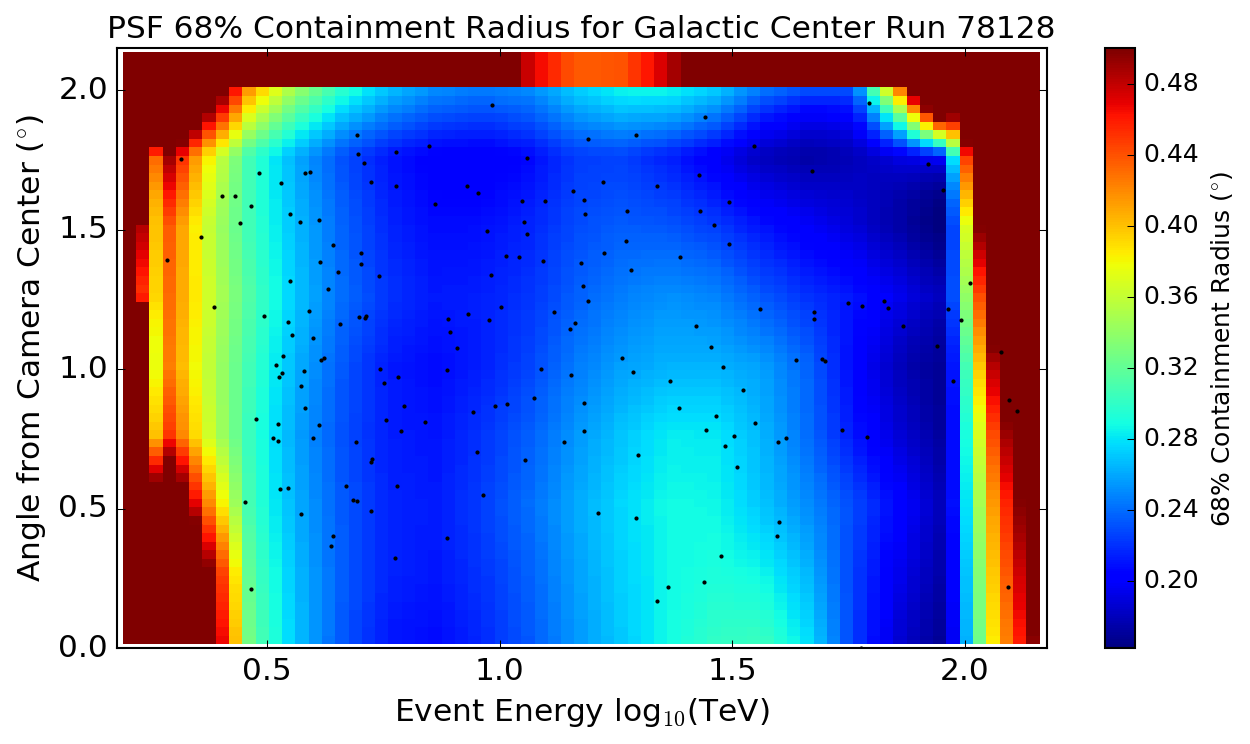
\includegraphics[width=\textwidth]{images/psf_king_plots/psf_parameter_space.eps}
      \caption[PSF Parameter Space]{
        The 68\% containment radius for the Energy/Offset parameter space for Galactic Center run 78128. 
        The green points show a subset of the event positions from that run in the parameter space.
      }
      \label{fig:psf_paramspace}
    \end{figure}

    For the Galactic Center and the Crab analyses, the distribution of 68\% containment radii for all events is shown in Figure \ref{fig:gc_psf_hist}.

    \begin{figure}[ht]
      \centering
      \includegraphics[width=0.85\textwidth]{images/psf_gc_eventhist/eventpsf.eps}
      \caption[Crab and Galactic Center Event PSFs]{
        The 68\% containment radius for all Galactic Center and Crab events used in this analysis.
      }
      \label{fig:gc_psf_hist}
    \end{figure}

  \subsection{Background Models}\label{background_production}
    A background model is a 3 dimensional function in camera X (in angle, parallel to azimuth), camera Y (in angle, parallel to elevation), and energy.
    The function calculates the number of observed events in the camera, per unit solid angle, unit time, and unit energy.
    This is used to quantify how many counts are expected when observing a gamma-ray-dark sky position, which estimates how many background proton events are being detected at different energies and in different parts of the camera.
    Understanding the background shape of the camera is crucial for properly studying extended sources, like dark matter halos, which may extend several degrees from the galactic center.
    Improperly estimating background models can result fake structures appearing around an astrophysical target.
    Background models with more than three dimensions are also possible, but require many more simulations, and are beyond the scope of this thesis.
    
    The background models used in this analysis are made from two background templates, one for each of the V5/V6 epochs.
    The templates are constructed from dark observations, detailed in \ref{veritasdata}.
    Each template is made by histogramming all background events by their energy, dividing by the bin width in MeV, and interpolating between bins to produce a spectral function.
    This spectral function can be seen in Figure \ref{fig:background_profile}.

    \begin{figure}[ht]
      \centering
      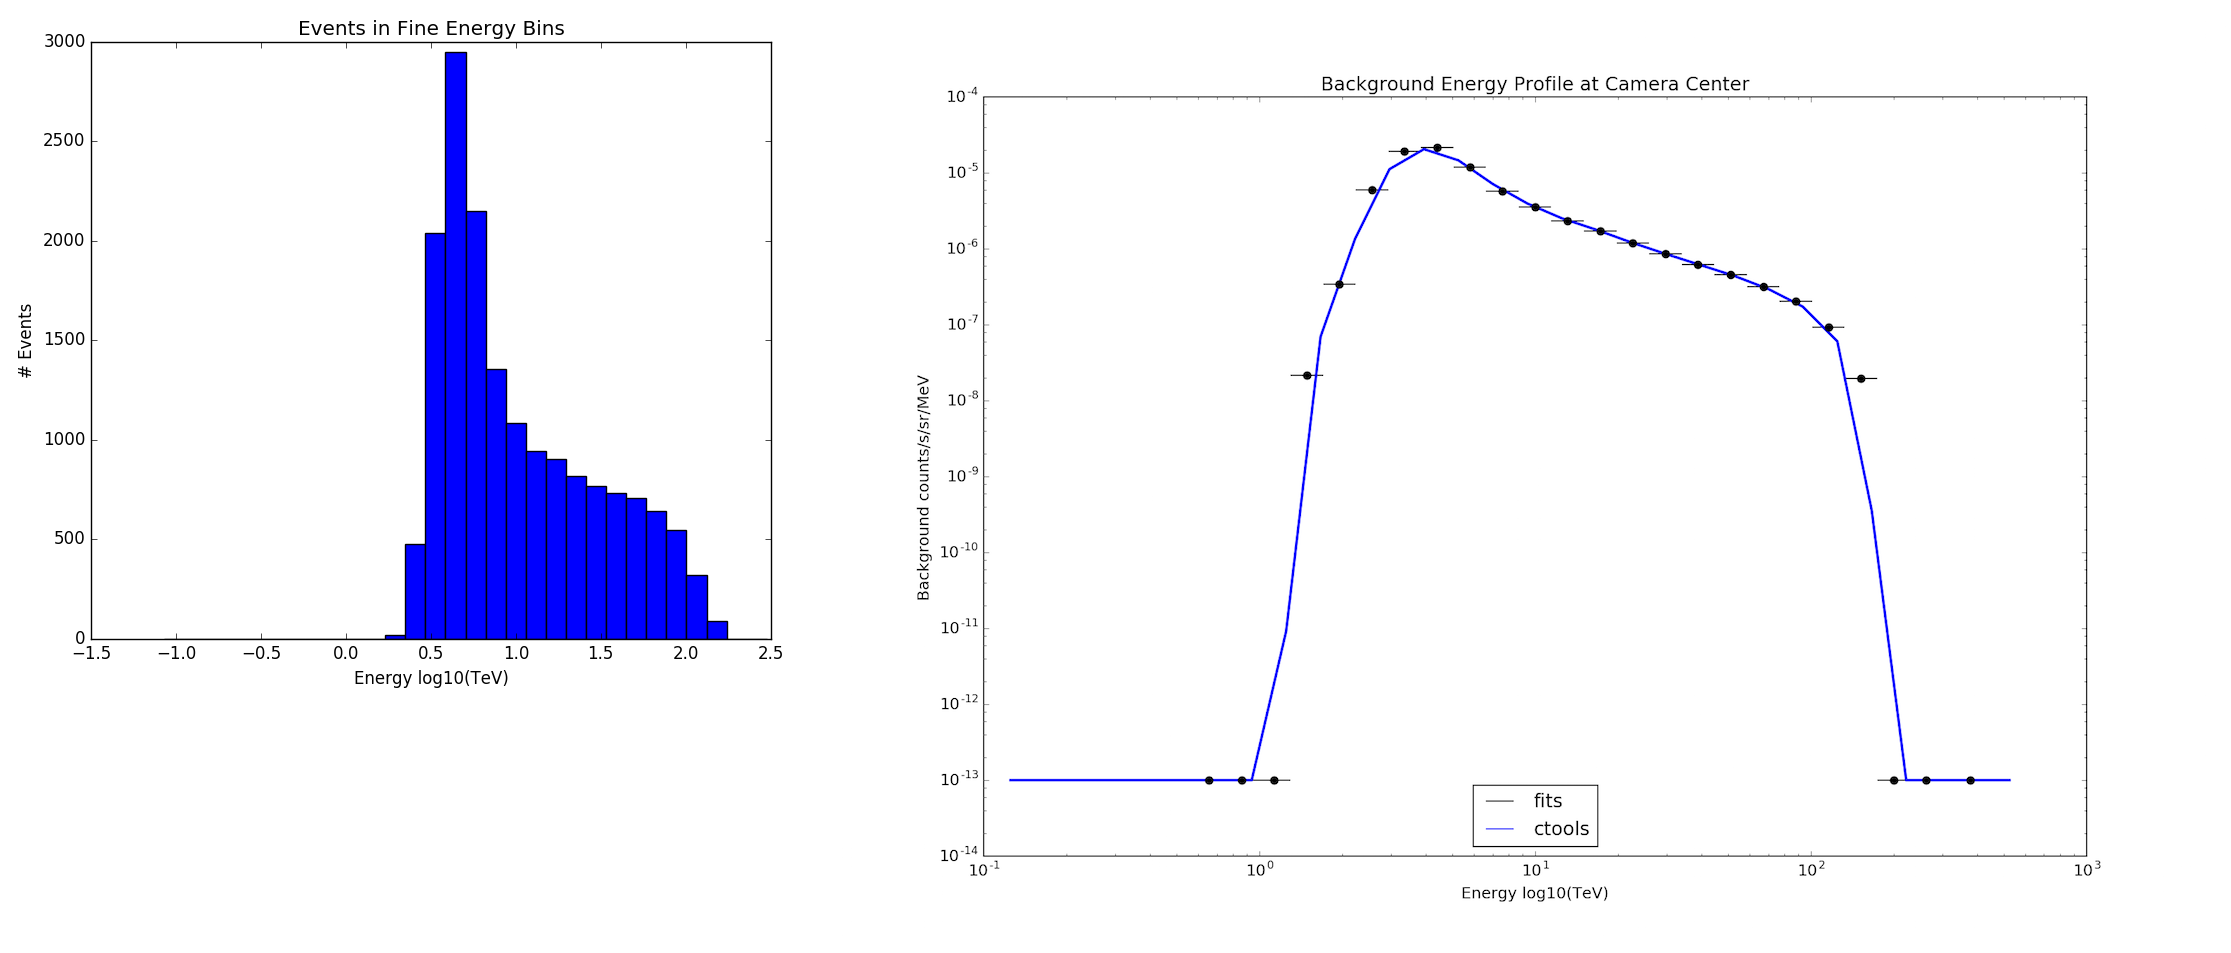
\includegraphics[width=0.7\textwidth]{images/ctools_background/background_construction.eps}
      \caption[CTOOLS Background Fine Energy Bins]{
        The V5 Background's fine-energy bins.
        The top plot shows the number of events in each fine-energy bin.
        The bottom plot shows the CTOOLS background values.
        The black lines show the fits background value and energy bin width saved to the background file, while the blue line shows the background value after CTOOLS loads and interpolates those fits background values.
      }
      \label{fig:background_profile}
    \end{figure}

    Then, the events are divided into high and low energies, and the events' reconstructed camera positions are binned radially about the camera center, with each bin divided by its bin area, producing two spatial functions.
    These high- and low-energy spatial functions are shown in Figure \ref{fig:background_radial}.
    
    \begin{figure}[ht]
      \centering
      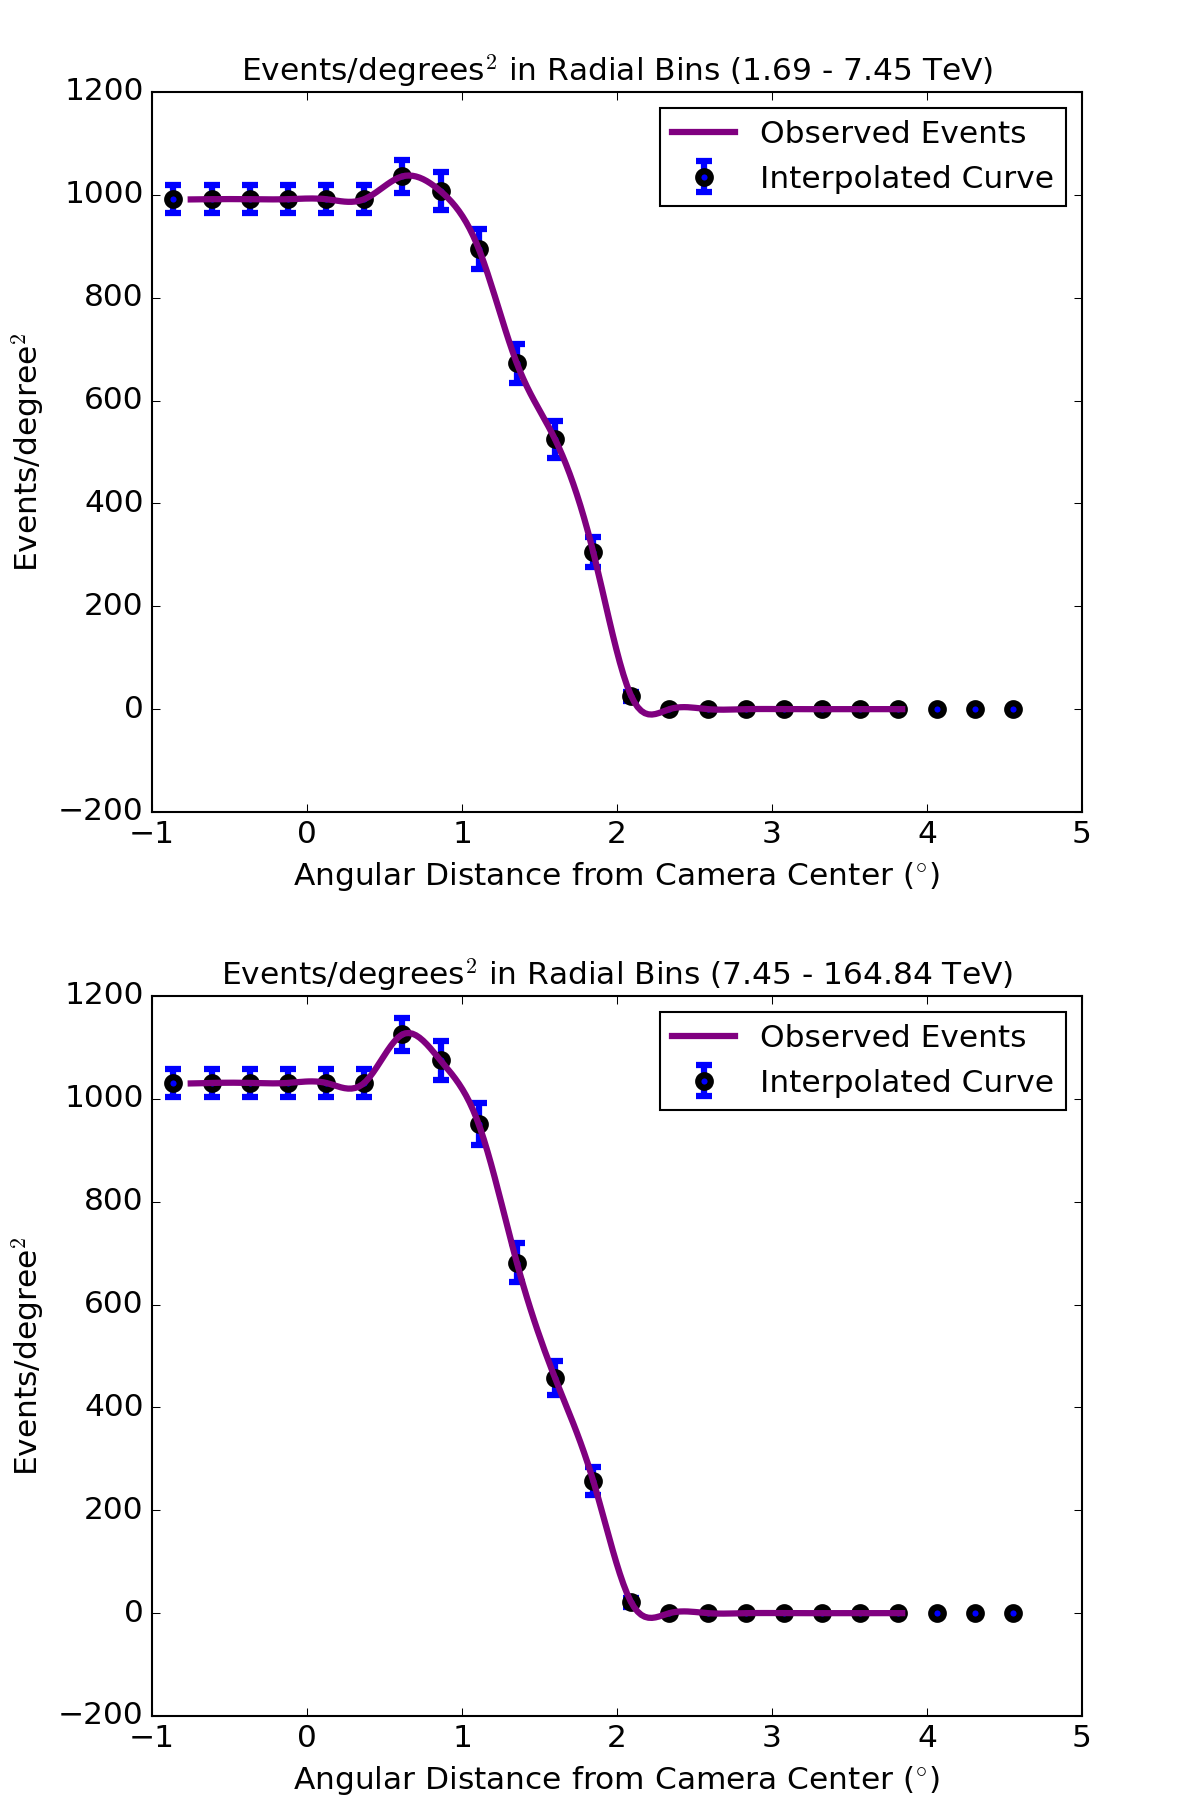
\includegraphics[width=0.7\textwidth]{images/ctools_background/radial_profiles.eps}
      \caption[CTOOLS Radial Background Profiles]{
        Radial bin profiles for the V5 background's two large-scale energy bins.
        The blue points are the counts per bin area, while the purple line is the interpolation with a spline interpolator of order 3 (see scipy.interpolate.interp1d())
        }
      \label{fig:background_radial}
    \end{figure}
    
    Finally, the spatial and spectral functions are multiplied together, as in Equation \ref{eqn:bck_template}.
    Interpolation is applied to keep the functions smooth between histogram bins, linearly in Camera X/Y, and linear-log${}_{10}$ in energy.
    
    \begin{equation}\label{eqn:bck_template}
      f(e,x,y) = A \times \textrm{spectral}(e) \times \textrm{spatial}(e,x,y) 
    \end{equation} 
    
    The function $f(e,x,a)$ has units of $\frac{\# Counts}{ \textrm{MeV} \times \textrm{s} \times \textrm{sr} }$
    The multiplied functions are then scaled with a constant $A$ such that the total integral of the template (integrating across Camera X, Camera Y, and Energy) matches the original number of counts in the dark runs, as in Equation \ref{eqn:background_template_function}.
    
    \begin{equation}\label{eqn:background_template_function}
      \textrm{\# Background Events} = A \times \int \textrm{spectral}(e) \times \textrm{spatial}(e,x,y) \times dx \: dy \: de
    \end{equation}

    This function $f(e,x,y)$ is the background template in Camera X/Y, which due to its radial symmetry can then immediatly be used as a CTOOLS background model in RA/Dec.
    Each background template is used in the likelihood analysis as a model multiplied by two free parameters, a normalization factor, and a power law spectral index.
    This lets the likelihood engine scale each run's background model up or down to best fit the events, so the background's absolute value is less important than the relative values in different parts of the camera or at different energies.

  \subsection{Energy Dispersion}\label{subsec:edisp}
    As events are reconstructed imperfectly, it is important to understand what the distribution of true energies are for a given reconstructed energy.
    In an analysis with CTOOLS, this is quantified by an energy migration matrix $E_{i,j}$, where $i$ denotes the $i^{\text{th}}$ reconstructed energy bin, and $j$ denotes the $j^{\text{th}}$ true energy bin.
    For true energy $j$, the distribution of reconstructed energies $f_{\text{reco}}$ is,

    \begin{equation}
      \label{eqn:edispreco}
      f_{\text{reco}}(j)=\frac{E_{i,j}}{ \sum_{i}E_{i,j} }
    \end{equation}

    for reconstructed energy $i$, the distribution of true energies $f_{\text{true}}$ is,

    \begin{equation}
      \label{eqn:edisptrue}
      f_{\text{true}}(i)=\frac{E_{i,j}}{ \sum_{j}E_{i,j} }
    \end{equation}

    By unfolding these distributions from the reconstructed energies, two significant effects are accounted for.
    The first is that the reconstruction software introduces biases in the event energy, meaning on average, an event at a given true energy is reconstructed at a higher or lower energy.
    The second effect that is accounted for is the dispersion in the reconstructed energies.
    Multiple simulations of the same energy event will result in a distribution of reconstructed energies.
    This has the effect of smearing out events in each energy bin of a spectra.
    In astrophysical spectra, which often follow an exponential curve, lower energy bins tend to have more events than the next highest energy bin, so smearing out the lower-energy bin contributes more to the higher-energy bin than the higher-energy bin contributes to the lower-energy bin.
    This has the effect that, when not accounted for, energy dispersion will harden observed astrophysical source spectra.
    In Figure \ref{fig:migmatrix}, a migration matrix is shown.

    \begin{figure}[ht]
      \centering
      \includegraphics[width=\textwidth]{images/edisp_plots/edisp.eps}
      \caption[Energy Migration Matrix]{
        An energy migration matrix used with Galactic Center run 82288.
        The reconstructed energy is on the x axis, and the true energy is on the y axis.
        The z (color) axis (why does the z axis have units of 1/s*MeV?? GCTAEdisp2D::operator() returns these units, but why??) denotes the number of simulated events that passed all cuts.
      }
      \label{fig:migmatrix}
    \end{figure}

\section{Camera Studies}
  The objective of this thesis is to put upper limits on the existance of a gamma-ray source that is both extended and faint.
  In order to better understand the effects that may impact the VERITAS camera behavior in the reconstruction software, several studies were performed.

  \subsection{Background Structure at the Low Energy Threshold}
    During the production of the initial background models, some new effects were noted.
    First, a series of gamma-like events were selected from observations with no known gamma-ray sources.
    These events were then divided into equal-statistics energy bins.
    For each equal-statistic energy bin, all the contained events were binned in camera X and Y.

    For a set of high-elevation observations, these backgrounds are shown in Figure \ref{fig:back_highelev}.
    It can be seen that all events are divided up into 3 equal-statistics energy bins in Figure \ref{fig:back_highelev}.A.
    Each energy bin is then binned in camera X and Y in Figure \ref{fig:back_highelev} B, C, and D.
    At these high elevations, the distribution of events in each energy bin is radially symmetric about the camera center.
    This happens because gamma ray's point of origin and its shower image in the camera are usually several tenths of a degree away from each other.
    In addition, the atmospheric mass-depth is similar in all parts of the camera.
    However, structures start to break the radial symmetry aat low energies and elevations.
    The cause of these structures is explored in the next section, \ref{subsubsec:diffusesims}.

    \begin{figure}[ht]
      \centering
      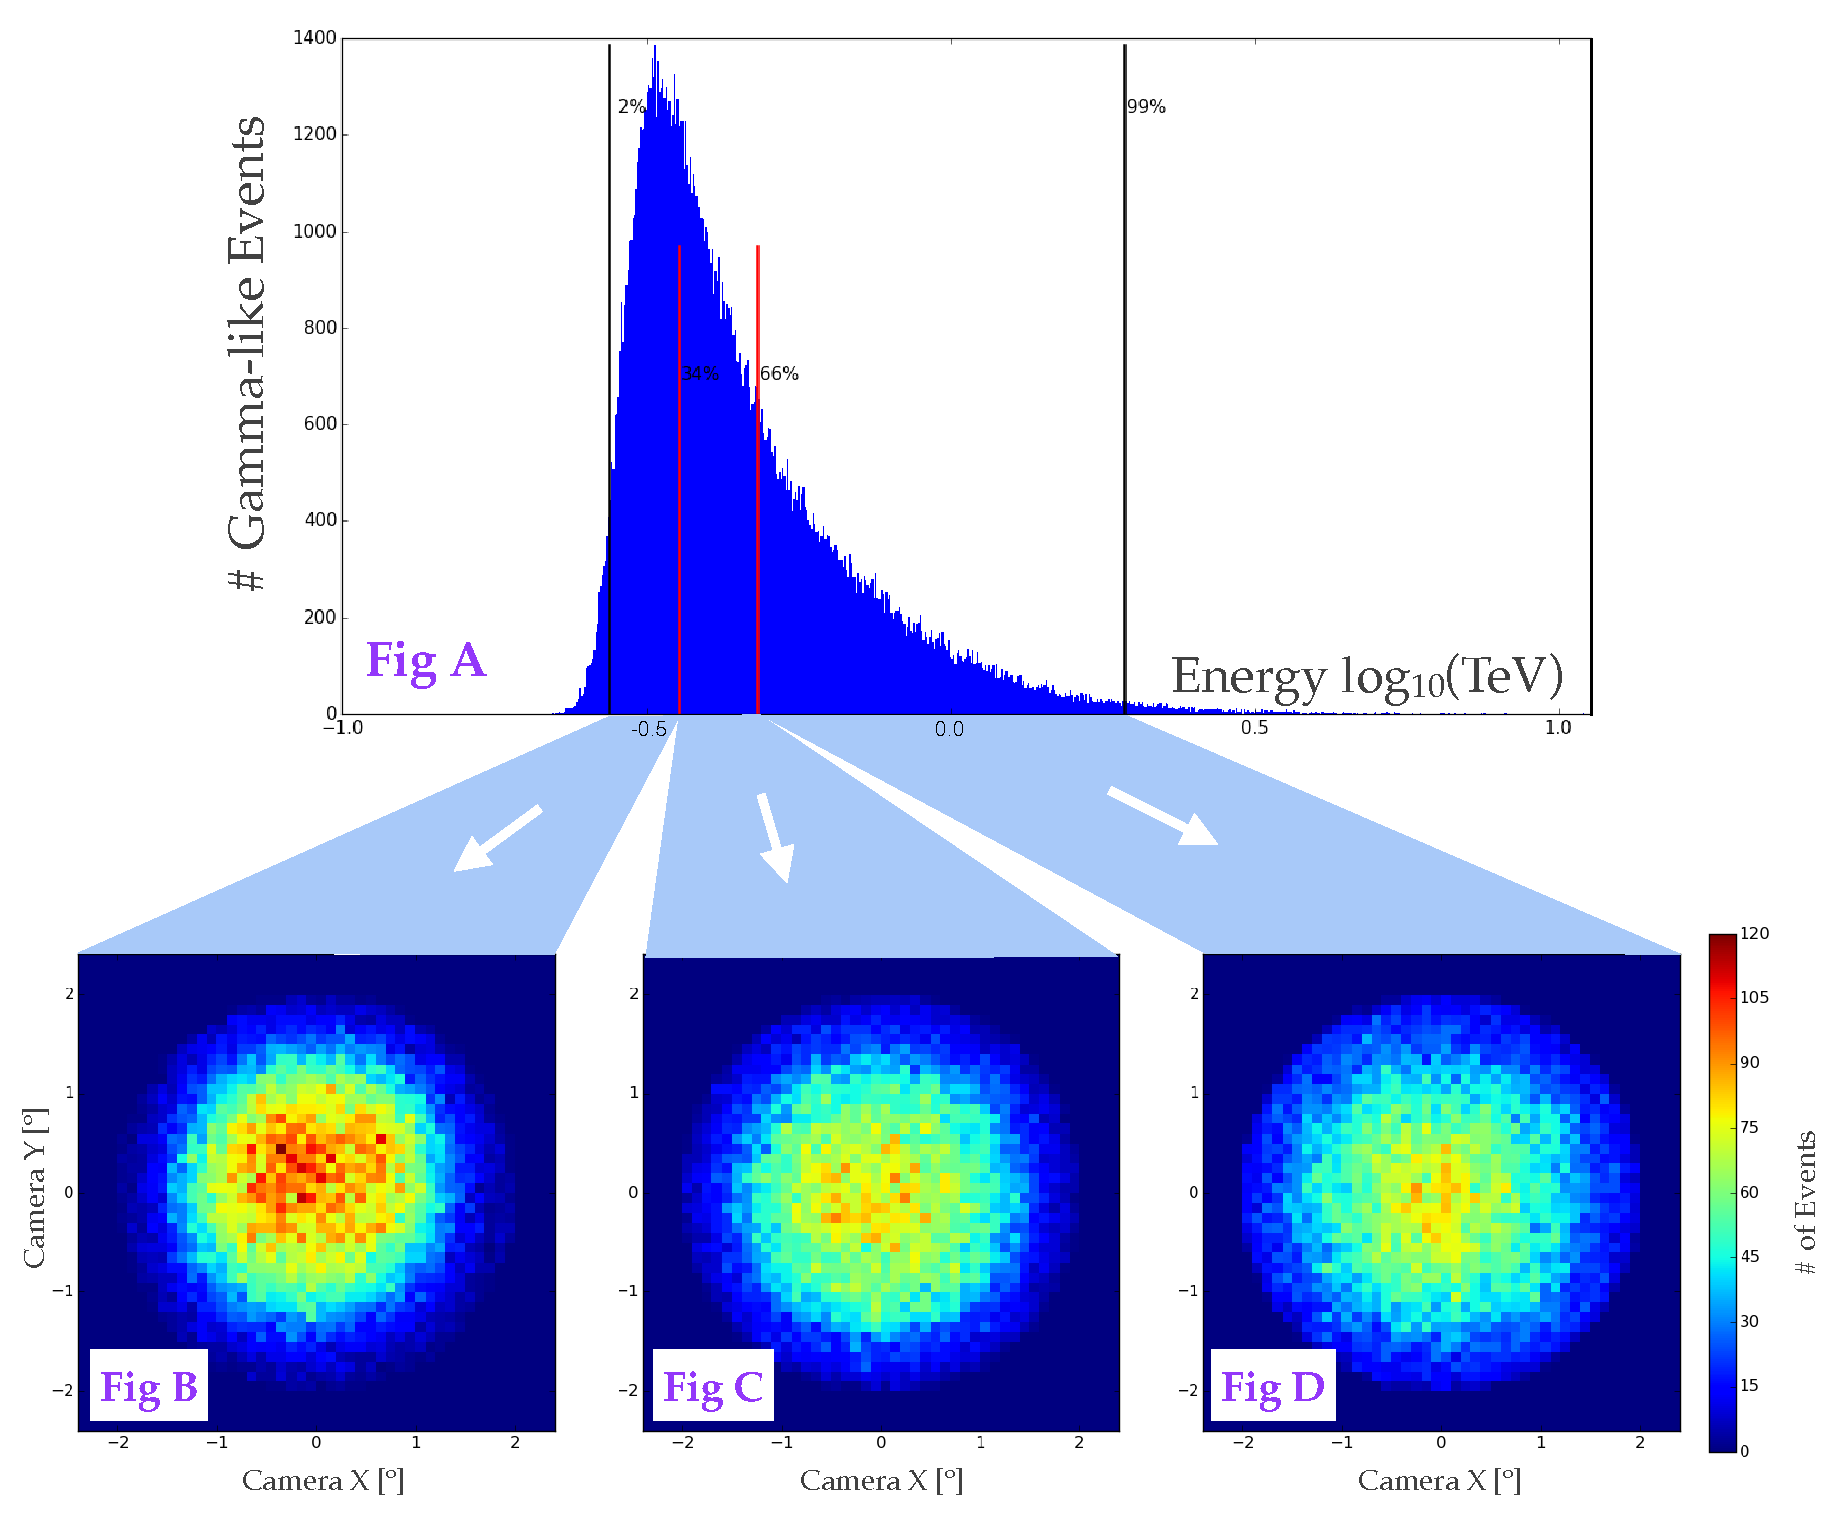
\includegraphics[width=\textwidth]{images/ctools/backgrounds_highelev.eps}
      \caption[FITS Background at \ang{50} Elevation]{
        Gamma-like Events from 52 observations (approximately \nicetilde20 hours) of M82, between \ang{50} and \ang{52} elevations.
        Events in Figure A are divided into 3 equal-statistics energy bins, and binned in Camera Coordinates in Figures B, C, and D.
      }
      \label{fig:back_highelev}
    \end{figure}

    In Figure \ref{fig:back_lowelev29} and Figure \ref{fig:back_lowelev26}, the same plots are constructed for a set of low-elevation (\nicetilde{}\ang{29} and \nicetilde{}\ang{26} respectivly) observations, using Galactic Center Off observations.
    These are again divided in to equal-statistic energy bins, and then each energy bin is binned in camera coordinates.
    It can be seen that in different energy bins, the background possesses different shapes.

    \begin{figure}[ht]
      \centering
      \includegraphics[width=\textwidth]{images/ctools/backgrounds_lowelev29.eps}
      \caption[CTOOLS Background at \ang{29} Elevation]{
        15 Sagittarius A* Off runs (\nicetilde7.5 observation hours), between elevations $ \ang{27.5} $ and $ \ang{30} $.
        Events are divided into 6 equal-statistics energy bins, of which four are binned in Camera Coordinates in Figures B, C, D, and E.
      }
      \label{fig:back_lowelev29}
    \end{figure}

    \begin{figure}[ht]
      \centering
      \includegraphics[width=\textwidth]{images/ctools/backgrounds_lowelev26.eps}
      \caption[CTOOLS Background at \ang{26} Elevation]{
        10 Sagittarius A* Off runs (\nicetilde5 observation hours), between elevations \ang{24} and \ang{27.5}. 
      }
      \label{fig:back_lowelev26}
    \end{figure}
  
  
  These effects are also noticeable in the galactic (l,b) event maps.
  In Figure \ref{fig:bkgvsel_crab}, the top plot shows the positions of all events, the middle histogram shows the distribution of event energies, and the bottom plot shows the event positions of events in a limited energy range, \SI{1.5}{\TeV}-\SI{3.25}{\TeV}.
  It it can be seen in the middle plot that this energy range is where more and more events are lost as energy decreases.
  When events are plotted in this limited energy range, it can be seen that there is a faint deficit along the bottom of the plot.

  When a similar series of plots are made for the galactic center in Figure \ref{fig:bkgvsel_sgra}, the effect is much stronger.
  In the top plot, events are radially symmetric about the source (there are differences due to the four wobble positions, but these are faint and not visible without quantification).
  But when only the events from \SI{1.5}{\TeV} to \SI{3.25}{\TeV} are plotted, a much clearer deficit is visible on the lower right part of the plot.
  This area corresponds to the deficit at bottom of the camera in Figures \ref{fig:back_lowelev29}.B and \ref{fig:back_lowelev26}.B
  It should be noted that there is a time-dependent rotation applied to go from the Camera X/Y (Earth Azimuth/Elevation) system to the Galactic (l,b) coordinates, which smears out the shape of the deficit, making it harder to notice in sky coordinates.
  
  This effect is important to this thesis because it implies that, at the lowest energies, the background rate is not radially symmetric.
  Radial backgrounds (sometimes referred to as acceptances) are typically used in VERITAS as they require less data to construct, and no other Camera X/Y or energy dependence had been demonstrated until now.
  As the analysis in this thesis only has a few hours of background observations (see table \ref{tab:observation_times}), only radially symmetric backgrounds templates/models could be constructed, which then required limiting the final analysis to $\geq\SI{4}{\TeV}$.
  
  \begin{figure}[ht]
    \centering
    \includegraphics[height=\textheight]{images/background_vs_elevation/background_vs_elevation_srccrab.eps}
    \caption[Background Vs Elevation Crab]
    {\small 
      Plots of Crab observations.
      Top: Skymap of all events.  Middle: Histogram of all events in energy.  Bottom: Skymap of events from \SI{1.5}{\TeV}-\SI{3.25}{\TeV}.  
      In the bottom plot, events from \SI{1.5}{\TeV}-\SI{3.25}{\TeV} are concentrated in the top half of the camera (before being rotated to galactic (l,b) coordinates), due to the air column density ($g/cm^2$) being \nicetilde20\% smaller at the top of the camera.
      (move some of this explaination to the regular text body??)
    }
    \label{fig:bkgvsel_crab}
  \end{figure}

  \begin{figure}[ht]
    \centering
    \includegraphics[height=\textheight]{images/background_vs_elevation/background_vs_elevation_srcsgra.eps}
    \caption[Background Vs Elevation Sgr A*]
    {\small 
      Plots of Sgr A* observations.
      Top: Skymap of all events.  Middle: Histogram of all events in energy.  Bottom: Skymap of events from \SI{1.5}{\TeV}-\SI{3.25}{\TeV}.  
      In the bottom plot, events from \SI{1.5}{\TeV}-\SI{3.25}{\TeV} are concentrated in the top half of the camera (before being rotated to galactic (l,b) coordinates), due to the air column density ($g/cm^2$) being \nicetilde20\% smaller at the top of the camera.
      (move some of this explaination to the regular text body??)
    }
    \label{fig:bkgvsel_sgra}
  \end{figure}

  

  \subsubsection{Diffuse Simulations}\label{subsubsec:diffusesims}
    To rule out any software causes, diffuse simulations were performed at similar energies and elevations.
    These consisted of 50,000 gamma rays at each of 1.4, 1.6, 2, and \SI{5}{\TeV}.
    The telescopes were fixed to an azimuth/elevation of (\ang{193},\ang{28}).
    The events themselves were distributed in a diffuse \ang{2.5}-radius disk.
    To approximate a simple gamma-hadron cut, any events with a mean-scaled-width falling outside the range of -2.0 to 0.5 were removed, which eliminates many of the showers that appear proton-like.
    These remaining gamma-like events are then binned in camera coordinates in Figure \ref{fig:back_simdiffuse}.


    \begin{figure}[ht]
      \centering
      \includegraphics[width=\textwidth]{images/backgrounds_diffuse_vs_data/backgrounds_sims/backgrounds_sims.eps}
      \caption[Diffuse Simulated Backgrounds]{
        Diffuse simulated gamma-like events in the camera coordinate system at a \ang{28} elevation, at 4 different initial energies.
      }
      \label{fig:back_simdiffuse}
    \end{figure}

    One can see that the ring and crescent structures persist in these diffuse simulations, implying these are physical effects of the atmosphere and camera, rather than a problem with the reconstruction software.
    (But what is the effect? I remember Gernot mentioning something about an edge effect? You should explain it here. --Orel??)

    This striking effect can be seen in Galactic Center data between certain energy ranges.
    As the plots are in galactic (l,b) coordinates, and there is a time rotation due to the Earth spinning on its axis, and observations are made at four wobble positions, the events clearly favor one half of the camera.
    
    These structures, and their strong dependency on both the energy and elevation of the telescopes may be a large factor in why the low-energy threshold regime of gamma-ray telescopes is poorly understood.
    Incorporating this effect into the instrument response functions would require modifying Event Display and CTOOLS, as well as creating another batch of diffuse simulations, with elevation increments of less than \ang{5}, all of which are computationally expensive.
    
    

  \subsection{Effect of Stars}
    As understanding the camera's background is important for extended source studies, i.e. dark matter halos, studies were performed examining the spatial effects of stars in the camera.
    It had been noted in the past that for visiual magnitude \nicetilde{}6 stars, the camera pixels they illuminated would have a higher average current.
    This translates into a higher pedvar in the affected pixels, which can decrease how often the pixel participates in shower images.
    In addition, if a star with magnitude brighter than 6 was in the field of view, it would cause high enough current in the pixel that it's voltage would be set to zero to prevent it from being damaged.
    For particularly bright stars (magnitude $\leq{}3$), often several pixels are disabled at a given time.
    (paragraph isn't consistant, needs checking??)

    A third effect is that, since the telescope camera is fixed to the ground, from the camera coordinate system, the sky rotates around the camera center.
    This means that over a single 30 min observation, any stars rotate around the camera center, disabling several camera pixels as it passes over them.
    The camera checks for these disabled pixels roughly once per minute by turning their voltage back on and monitoring the current, and setting it back to zero if the current is still above the threshold.

    These effects imply that to study the effect of stars, one must study the effect of high-current and disabled camera pixels, and use this information to construct the effect of stars.
    In this section, the effects of disabled camera pixels are studied.

    % see calculations/disabledpixel_obstime , those 250 crab runs turned into about 13.5 observation hours
    To examine the effects of disabled pixels, \nicetidle13 hours of Crab observations were analyzed twice with Event Display.
    The first analysis was with the default analysis chain settings, and the second time with a single pixel disabled in all four telescopes.
    This mimics the effect of having a star in the field of view that is bright enough to disable a pixel.

    After both sets of events are passed through gamma-hadron cuts, they are compared.
    These two sets of events were examined for events that disappeared when the pixel was disabled, as well as for new events that appeared.
    Events that are still present in both event lists can then be tested to see how far their reconstructed position moved in the camera.

    In Figure \ref{fig:dpix_rel_camera}, the relative event rate in the camera is plotted when pixel 115 is disabled in all four telescopes.
    This relative event rate is calculated by taking, for each bin, the number of reconstructed gamma-like events, divided by the pixel-enabled number of reconstructed events.
    It can be seen that there is a loss of events near the disabled pixel (the black circle), with a rate closer to 100\% the further away one goes from the disabled pixel.

    \begin{figure}[ht]
      \centering
      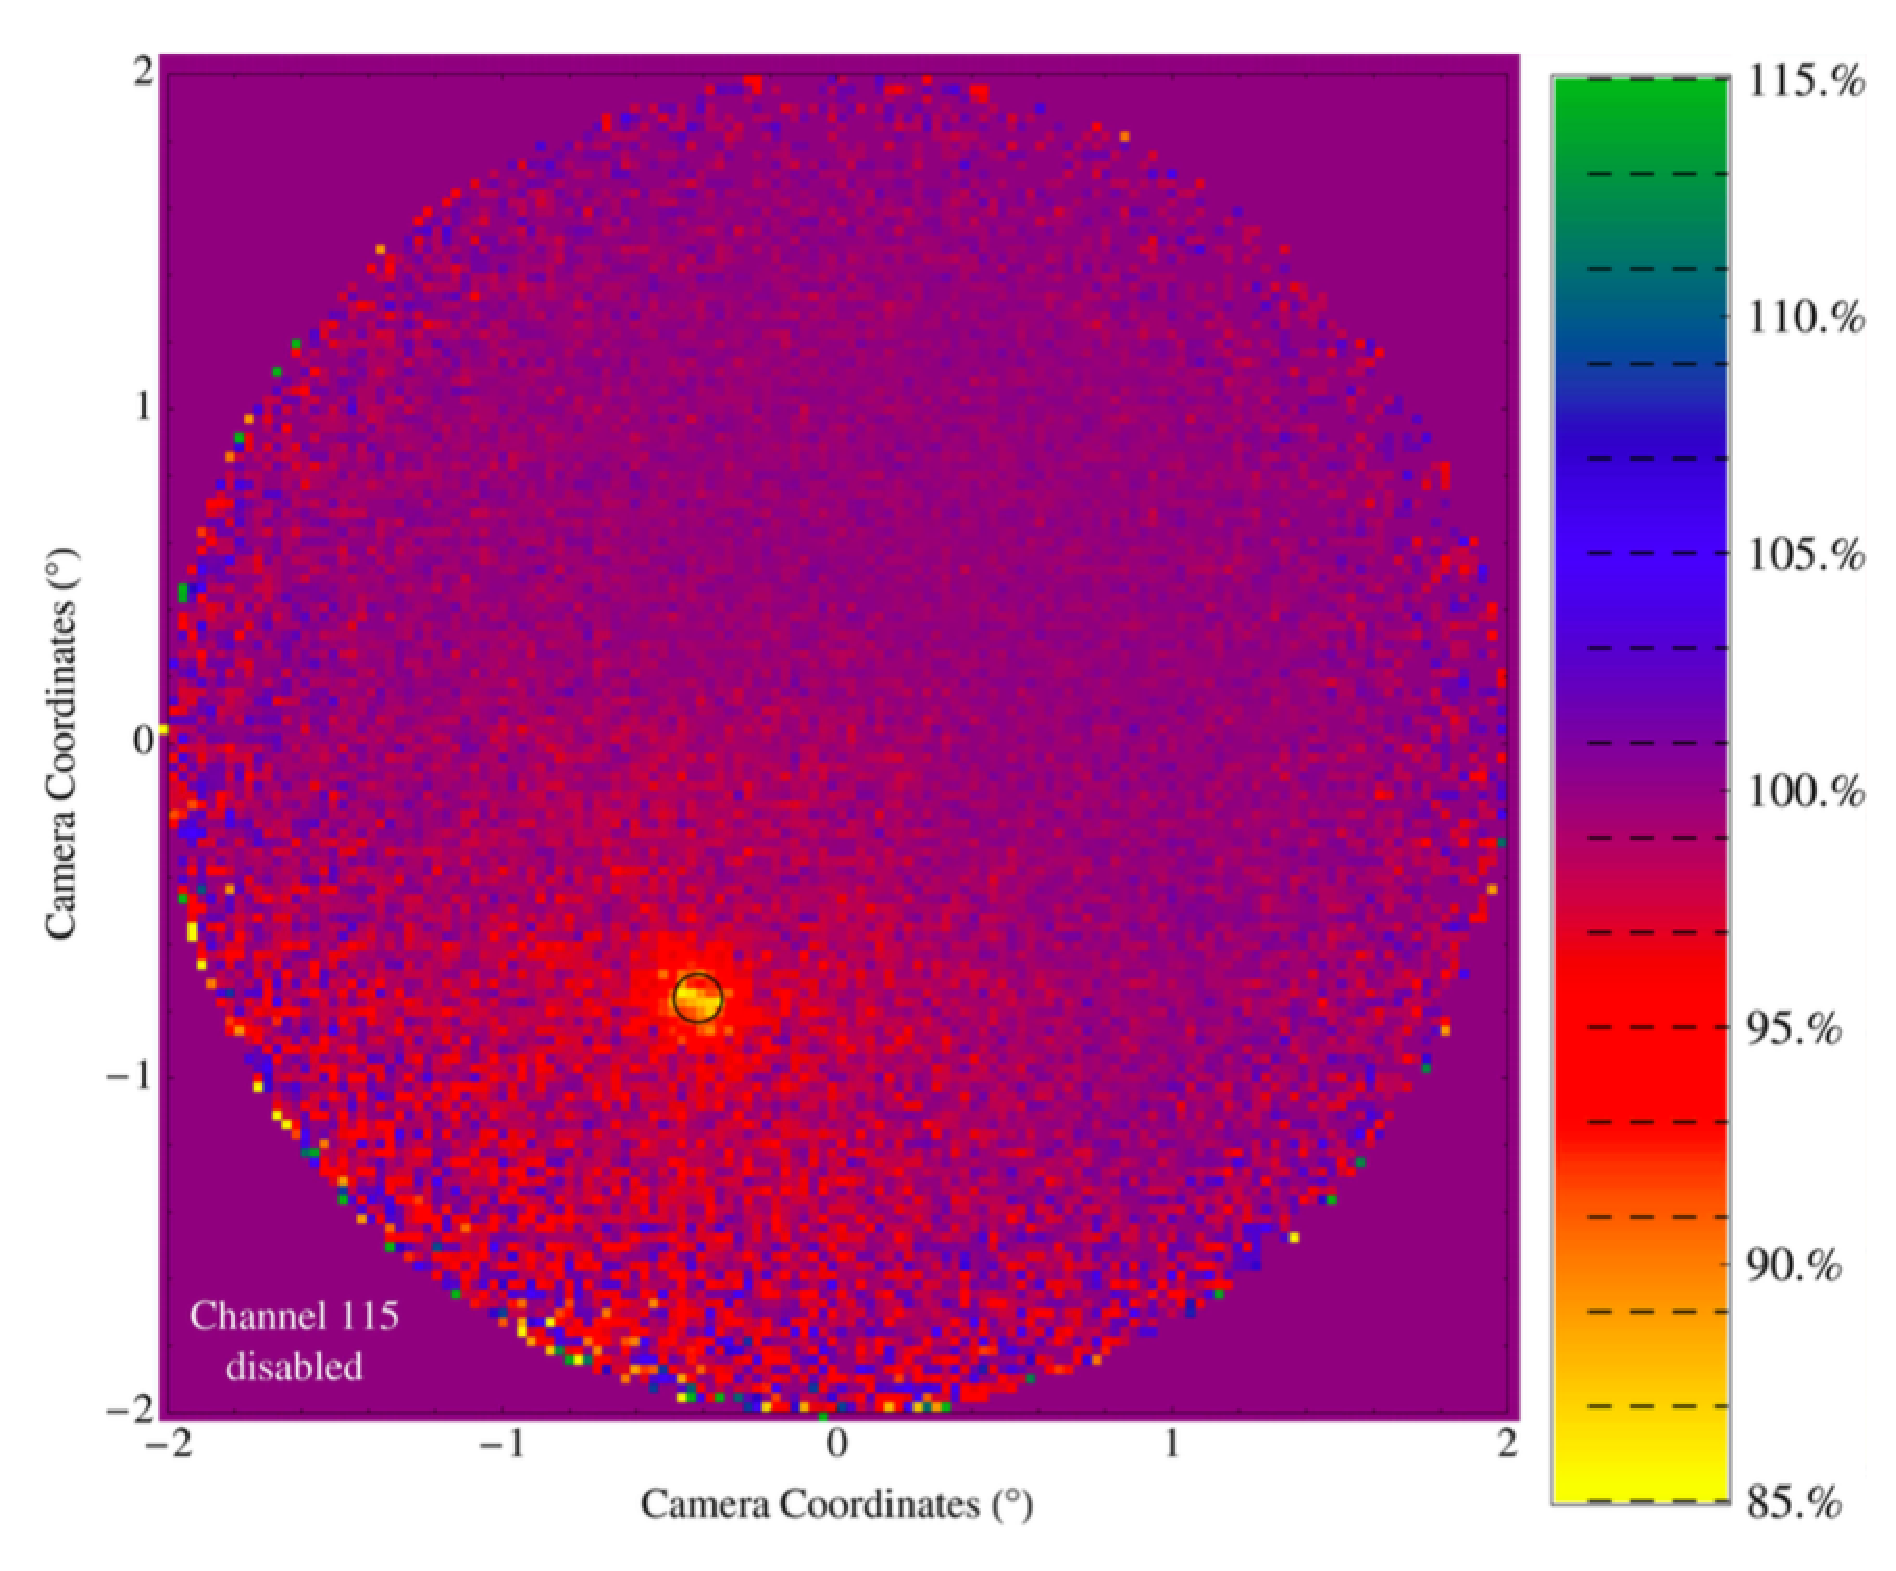
\includegraphics[width=0.8\textwidth]{images/disabled_pixel/relativerate_camera}
      \caption[Relative Event Rate]{
        Event rate in the camera with pixel 115 disabled (denoted by the black circle) in all four telescopes, relative to having all pixels enabled.
        Camera coordinate axes are parallel to azimuth and elevation.
      }
      \label{fig:dpix_rel_camera}
    \end{figure}

    In Figure \ref{fig:dpix_rel_radial}, the bin values from Figure \ref{fig:dpix_rel_camera} are divided into radial bins centered around the disabled pixel.
    The average relative event rate is then calculated for each bin, along with a 1-sigma distribution width for the error bars.
    It can be seen that there are three distinct regions to the plot.
    (How do you actually calculate the uncertainties here? If you take a ratio between numbers of events, you need to calculate the uncertainty explicitly since there are many events which are common to both bins and they shouldn't be counted twice in the uncertainty.  This is important as it affects the conclusion you reach below. --Orel??)
    In the first region, from radius $\ang{0}$ to $\ang{0.3}$, the relative event rate starts extremely low, and rises rapidly.
    In the second region, from radius $\ang{0.3}$ to $\ang{1.6}$, the relative event rate is still rising, but much more slowly.
    In the third region outside $\ang{1.6}$, there is almost no effect.

    ??This discussion of three regions is not really correct and not entirely relevant.
    It does not give a conclusion on what you do with this information.
    The simplest idea would be to apply a correction to events with disabled pixels based on this plot. Do you that? If not, why not? If yes, it should be mentioned here.
    There are really only two “regions” in this plot, one where you lose events and need to correct for that and one where the ratio is 100% within uncertainties.
    Here is where the correct calculation of uncertainties of the ratio becomes important.
    I think as it is, you might be overestimating the uncertainties, which would result in a larger systematic uncertainties from this correction, if you apply it. --Orel??


    \begin{figure}[ht]
      \centering
      \includegraphics[width=\textwidth]{images/disabled_pixel/relativerate_radial}
      \caption[Radial Relative Event Rate]{
        Same relative event rate as in Figure \ref{fig:dpix_rel_camera}, but averaged into radial bins, centered on the disabled pixel 115.
      }
      \label{fig:dpix_rel_radial}
    \end{figure}

    In Figure \ref{fig:dpix_disappear}, the positions of events that were rejected by cuts are shown.
    The white area indicates many events are lost in the area of the disabled pixel.
    These events would have smaller images, and would be much more susceptable to being cut.

    \begin{figure}[ht]
      \centering
      \includegraphics[width=0.8\textwidth]{images/disabled_pixel/disappearing_events}
      \caption[Disappearing Events]{
        Positions of events that disappeared when pixel 115 was disabled in all four telescopes.
        Positions are from their pixel-enabled reconstructed position.
      }
      \label{fig:dpix_disappear}
    \end{figure}

    In Figure \ref{fig:dpix_appear}, the positions of events that are now able to pass cuts are shown.
    It should be noted that these are not events that these are events 'created' by disabling a pixel.
    Rather, they are events that, with the pixel enabled, did not pass cuts.
    Now that the pixel is disabled, they do pass cuts.

    What is also noticeable is that the highest concentration of lost events was in the pixel's area, whereas the highest rate for appearing events is actually in a ring with a radius of \nicetilde1.5 pixels around the disabled pixel.
    This is probably due to the fact that disabling a pixel can make some images look thinner or wider, depending on where the disabled pixel is in the image.
    A thinner image will look more gamma-like, making it more likely to pass cuts, appearing like 'new' events.
    On the other hand, a wider image looks more hadron-like, and is less likely to pass cuts, causing some events to disappear.

    \begin{figure}[ht]
      \centering
      \includegraphics[width=0.8\textwidth]{images/disabled_pixel/appearing_events}
      \caption[Newly Appearing Events]{
        Positions of new events that appeared when pixel 115 was disabled in all four telescopes.
        Positions are from their pixel-disabled reconstructed position.
      }
      \label{fig:dpix_appear}
    \end{figure}

    In Figure \ref{fig:dpix_move}, the movment of gamma-like events is shown, when pixel 115 was disabled in all four telescopes.
    Only events which moved more than $0.1*psf$ are shown.
    It should be noted that relatively few (\nicetilde{}100 in the 20-minute-long run 53703) events move more than this, and the events that do move are mostly ones with non-compact image shapes that are amputated when a pixel is disabled.

    What can be learned from this is that while only a small number of events' positions depend on a given pixel, pixels can have an impact on the reconstructed position from halfway across the camera.
    This may imply that the event PSF is, to second order, dependent on the number of disabled pixels, though no studies were done to confirm this.


    \begin{figure}[ht]
      \centering
      \includegraphics[width=0.8\textwidth]{images/disabled_pixel/moving_events}
      \caption[Event Movement]{
        Positions of events that moved when pixel 115 (denoted by the red circle) was disabled in all four telescopes.  
        Arrows point from the pixel-enabled position to the pixel-disabled position.
      }
      \label{fig:dpix_move}
    \end{figure}

    As the acceptance for a particular event and the event's effective area are strongly related, the loss of acceptance also means a loss of effective area in the area of this pixel.
    This can have effects on the energy reconstruction.
    Additionally, for CTA and its projected \ang{7}-diameter field of view, more stars will be in the field of view, implying there will be more camera pixels affected by their light.

    Future studies could also compare how events move in energy when a pixel is disabled.
    Another study might investigate how the reconstructed shower-telescope distance changes, since a shower with fewer pixels will look further away, and may be reconstructed differently.
    In general, as a pixel is disabled, it is expected that lower energy events and showers further away will be more vulnerable, and will show stronger differences than higher energy events or closer showers.



%% \cleartooddpage[\thispagestyle{empty}]
\chapter{The Galactic Center}

\section{The Supermassive Black Hole}

\section{Diffuse Emission}

\section{Nearby Astrophysical Sources}

\cleartooddpage[\thispagestyle{empty}]
\newcommand{\Like}{L}
\newcommand{\LogLike}{\mathcal{L}}
\newcommand{\LogLikeMax}{\LogLike_{\textrm{max}}}
\newcommand{\xtrue}{\mathbf{x }}
\newcommand{\xdet }{\mathbf{x'}}
\newcommand{\ltrue}{\mathbf{l }}
\newcommand{\ldet }{\mathbf{l'}}
\newcommand{\btrue}{\mathbf{b }}
\newcommand{\bdet }{\mathbf{b'}}
\newcommand{\Etrue}{\mathbf{E }}
\newcommand{\Edet }{\mathbf{E'}}
\newcommand{\ttrue}{\mathbf{t }}
\newcommand{\tdet }{\mathbf{t'}}
\newcommand{\Aeff }{A_\textrm{eff }}
\newcommand{\Edisp}{E_\textrm{disp}}
\newcommand{\Mnull}{M_\textrm{null}}
\newcommand{\Malt }{M_\textrm{alt }}

\chapter{A Likelihood Search for Dark Matter}\label{chapter:analysis}

\section{Veritas Data}\label{veritasdata}
  The analysis in this thesis relies on three sets of VERITAS data.
  One set contains observations of the Crab Nebula, and another of the Galactic Center.
  A third set contains observations of a dark region \nicetilde\ang{5} away from the Galactic Center.
  This dark region is referred to as  Sgr A* Off, and is located at (l,b)=(\ang{357.3396}, \ang{3.9984}).
  Sgr A* Off is located a few degrees away to avoid the bright diffuse gamma-ray emission caused by the galactic plane.
  The Galactic Center and Sgr A* Off observation regions are shown in Figure~\ref{fig:gcfieldsofview}.
  To quantify the detector efficiency, observations are taken at \ang{0.5} or \ang{0.7} offsets from each observing target, in four different directions (wobbles) along right ascension/declination axes.

  \begin{figure}[ht]
    \centering
    \includegraphics[width=0.95\textwidth]{images/skypointings/plot.pdf}
    \caption[VERITAS Galactic Center Pointings]{
      Fields of view for Galactic Center observations.
      Each circle marks the detection area of one telescope pointing.
      Green circles are Galactic Center observations, while dark blue circles are the Sgr A* Off observations used to construct the camera-background templates.
      The light blue band is the galactic plane.
    }
    \label{fig:gcfieldsofview}
  \end{figure}

  All three sets of data include observations from both the V5 and V6 epochs (see Section~\ref{sec:epochs}).
  All used data was taken from April 2010 to June 2016.
  The specific VERITAS data run numbers are listed in Appendix~\ref{app:runlists}.

  \begin{table}[]
    \centering
    \caption{Hours of observations taken at each source/epoch combination.}
    \label{tab:observation_times}
    \begin{tabular}{|l|l|l|l|}
      \hline
      \textbf{Epoch} & \textbf{Crab} & \textbf{Sgr A*} & \textbf{Sgr A* Off} \\ \hline
      V5             & 3.3           & 46.3            & 13.0                \\ \hline
      V6             & 5.5           & 62.7            & 4.7                 \\ \hline
      % times calculated with $VERIPY/thesis/plots/obs_times.py
    \end{tabular}
  \end{table}


  \begin{figure}[ht]
    \centering
    \includegraphics[width=0.95\textwidth]{images/data_elevation_plots/plot.pdf}
    \caption[VERITAS Data Elevation Exposure]{
      Camera center elevation for the three sets of data.
      The three peaks in the Sgr A* data are from the 4 wobble positions being at different elevations.
      The North wobble observations peak at elevation \nicetilde\ang{29.75}, East and West wobbles observations at \nicetilde\ang{29.25}, and South wobble observations at \nicetilde\ang{28.75}.
    }
    \label{fig:datapointingelevations}
  \end{figure}

  There are comparativly fewer Sgr A* Off observations because this source is only used for background estimation, and telescope time is in high demand.
  There are also fewer Crab observations, as the majority of its data is taken at higher elevations, where the telescope has increased sensitivity to lower energies.
  
  For all of these observations, quality cuts were applied.
  This includes monitoring the telescope hardware and cloud ceiling in the field of view.
  Two far-infrared Pyropemeters are used to measure the cloud ceiling height, by measuring the temperature of the sky.
  With the pyrometer, clouds are significantly warmer (\nicetilde\ang{50} C) than clear sky.
  Low-quality segments of data, where there are large (>20\%) and/or rapid (<=\SI{30}{s}) changes in the L3 trigger rate or cloud ceiling height, are removed from the analysis~\cite{bird_weather}.
  % see Bird 2015 thesis pg 55

  Because each VERITAS epoch has a different hardware configuration, they also each have their own separate set of effective areas, point spread functions, energy migration matricies, and camera background models.
  In addition, specific IRFs were calculated for additional data dimensions, including the frequency of night sky background photons in the camera, the telescope elevation, the event energy, and each event's distance from the camera center.
  
  After this data is collected, it is used in a likelihood analysis, detailed in the next section.

\section{Likelihood Ratio Test}\label{sec:likeratio}
  A likelihood ratio test determines which of two model groups is a statistically better fit to a set of data.
  It is performed by calculating, for a group of events, the likelihood of detecting that group of events for each of two model groups.
  Once the likelhood is calculated, then the parameters of the model are varied until the maximum likelihood is found for each model.
  These two maximum likelihoods can then be used to calculate the test statistic (TS), which determines which model is statistically favored, and to what degree it is favored.
  
  \subsection{Likelihood Calculation}
  At its heart, a likelihood is a product of probabilities.
  With two events, the likelihood is $(\textrm{probability that event 1 happens})\times(\textrm{probability that event 2 happens})$.
  In a counting experiment like VERITAS, the likelihood $\Like$ is determined via poissonian statistics, shown in Equation~~\ref{eqn:simple_like}.
  In this equation, $n$ is the number of observed events, and $m$ is the average number of events predicted by a model group.
  
  \begin{equation}\label{eqn:simple_like}
    \Like = \frac{e^{-m} m^n}{n!}
  \end{equation}
  
  For increased statistical power, the VERITAS data can be split into bins in energy, galactic l and b, and time.
  When combining multiple bins arbitrarily ordered by index $j$, each bin's likelihood is multiplied together as in Equation~\ref{eqn:simple_like_2}.
  These events could be binned in dimensions of sky position, energy, time, or other event parameters, or any combination of these parameters.
  Future likelihood calculations may also include shower core position on the ground, or distance to the shower, or other observables.
  
  \begin{equation}\label{eqn:simple_like_2}
    \Like = \prod_j \frac{ e^{-m_j} \; m_{j}^{n_j}}{n_{j}!}
  \end{equation}

  Equation~\ref{eqn:simple_like_2} is a general formula for calculating a binned likelihood of poissonian events.
  As events are grouped by bins, some information is lost, which generally results in a less powerful ratio test.
  The result in Equation~\ref{eqn:simple_like_2} can be expanded into an unbinned likelihood through the following derivation.
  First, Equation~\ref{eqn:simple_like_2} can be rearranged:
  
  \begin{equation}\label{eqn:simple_like_3}
    \Like = \prod_j e^{-m_j} \prod_j \frac{m_j^{n_j}}{n_{j}!}
  \end{equation}
    
  \begin{equation}\label{eqn:simple_like_4}
    \Like = e^{- \sum_j m_j} \prod_j \frac{m_j^{n_j}}{n_{j}!}
  \end{equation}
  
  Then, the size of each bin can be shrunk until there are only 1 or 0 events in each bin.
  For empty bins (where $n=0$), the product in Equation~\ref{eqn:simple_like_4} becomes
  
  \begin{equation}\label{eqn:simple_like_4a}
    n=0 \rightarrow \frac{m_j^{n_j}}{n_j!} = \frac{m_j^{0}}{0!} = \frac{1}{1} = 1 .
  \end{equation}

  For bins with 1 event, the product in Equation~\ref{eqn:simple_like_4} becomes

  \begin{equation}\label{eqn:simple_like_4b}
    n=1 \rightarrow \frac{m_j^{n_j}}{n_j!} = \frac{m_j^1}{1!} = \frac{m_j}{1} = m_j = m_i ,
  \end{equation}

  where $i$ is the $i^{\textrm{th}}$ event, and $m_i$ is the number of predicted events at event $i$'s sky position, energy, and time.
  In this derivation, $m_j$ converts to $m_i$, because all the $n=0$ bins are now 1 and can be ignored, so a loop over the $j$ bins becomes a loop over the $i$ events.
  Then Equation~\ref{eqn:simple_like_4} becomes Equation~\ref{eqn:simple_like_5}.
  
  \begin{equation}\label{eqn:simple_like_5}
    \Like = e^{- \sum_j m_j} \prod_i m_i
  \end{equation}
  
  In Equation~\ref{eqn:simple_like_5}, $\prod_i m_i$ encodes the data events, while $\sum_j$ encodes the model information.
  When calculating $\Like$, certain computational problems can arise.
  Calculating the product of many small probabilities can result in extremely small numbers, beyond the binary storage limit of common variable types.
  Calculating derivatives of some of these numbers is computationally expensive, so to solve these two problems, the log-likelihood $\LogLike$ is instead calculated.
  
  \begin{equation}\label{eqn:simple_like_6}
    \LogLike = \textrm{log} \left ( \Like \right ) 
  \end{equation}
  
  This is possible because both $\Like$ and $\LogLike$ are both strictly increasing functions, so the maximum of both will be at the same position in the parameter space.
  The log-likelihood for a group of bins is then:
  
  \begin{equation}\label{eqn:simple_like_7}
    \LogLike = \textrm{log} \left ( e^{- \sum_j m_j} \prod_i m_i \right ) = - \sum_j m_j + \sum_i \textrm{log} \left ( m_i \right )
  \end{equation}
  
  When the bin size is infinitely small, $m_i$ becomes $P_i$, the value of the probability density function (of all models combined) at the position of the event, as in Equation~\ref{eqn:simple_like_8}.
  
  \begin{equation}\label{eqn:simple_like_8}
    \LogLike = \textrm{log} \left ( e^{- \sum_j m_j} \prod_i m_i \right ) = - \sum_j m_j + \sum_i \textrm{log} \left ( P_i \right )
  \end{equation}
  
  The unbinned Equation~\ref{eqn:simple_like_8} shows how the log-likelihood is calculated in this analysis.
  The $\sum_{j} m_{j}$ term can be interpreted as the total number of events predicted by all models, sometimes referred to as $N_{pred}$.
  Please note however, that while a binned likelihood calculation scales with the number of bins (and some lost information), the unbinned likelihood calculation scales with the number of events, which can lead to large likelihood maximization times (see later in this section).
  
  \subsection{Models}\label{sec:model_irf_folding}
  
  Models are used in a likelihood analysis to predict the number of events that a particular source deposits into a particular bin.
  In a likelihood analysis, each source of events gets its own model.
  Each model is described by a function $M$, and different sources will have different $M$ functions.
  The function $M$ has dimensional units of $\frac{\textrm{counts}}{\textrm{energy}\times\textrm{solid angle}\times\textrm{area}\times\textrm{time}}$.
  This function can be integrated over the energy, sky, and time region covered by a bin to calcuate the number of events predicted in that bin, as shown by Equation~\ref{eqn:model_int}.
  
  \begin{equation}\label{eqn:model_int}
    m_{i \, \textrm{or} \, j} = \int_{t\,\textrm{bin}} \int_{E\,\textrm{bin}} \int_{b\,\textrm{bin}} \int_{l\,\textrm{bin}} M(l,b,E,t)\; dl \; db \; dE \; dt
  \end{equation}
  
  In this equation, $l$ and $b$ are sky coordinates, $E$ is energy, and $t$ is time.
  The basic models used in this analysis can be broken apart into their spatial, spectral, and temporal components, as in Equation~\ref{eqn:modelparts}.

  \begin{equation}\label{eqn:modelparts}
    M(l,b,E,t) = M_s(l,b,E,t) \; \; M_e(l,b,E,t) \; \; M_t(l,b,E,t)
  \end{equation}
  
  For this thesis, the sources being modeled are either constant in flux, or in equilibrium, so time-dependent effects are ignored by setting $M_{t}(l,b,E,t) = 1$.

  For a basic point source, the spatial model function $M_s$ is shown in Equation~\ref{eqn:pntsrc_Ms}.

  \begin{equation}\label{eqn:pntsrc_Ms}
    M_{s,\textrm{point}}(l,b,E,t) = \lim_{a\to\infty} \frac{1}{ \abs{a} \sqrt{\pi} } e^{ - \left ( \sqrt{ (l-l_o)^2 + (b-b_o)^2 }/a \right )^2 }
  \end{equation}
  
  In this equation, $l_o$ and $b_o$ specify the position of the point source in Galactic sky coordinates, which can be model parameters.
  More complex $M_s$ functions may also have the spatial structure depend on energy $E$ or time $t$, or may take on other spatial shapes like an ellipse or a radially-symmetric profile.
  The energy spectrum can be similarly modeled by a basic power law.
  This basic power law is defined by the model function $M_e$, and is shown in Equation~\ref{eqn:powerlaw_Me}.
  
  \begin{equation}\label{eqn:powerlaw_Me}
    M_{e,\textrm{powerlaw}}(l,b,E,t) = N_o \left ( \frac{E}{E_o} \right )^{-\gamma}
  \end{equation}

  In this equation, $N_o$ is the flux normalization, $E_o$ is the pivot energy, and $\gamma$ is the spectral index, which can all be model parameters.

  
  \subsection{Instrument Response Function Folding}\label{subsec:folding}
  The average number of counts predicted by a model is calculated by integrating over the entire energy, sky, and time regions in the analysis.
  Because the reconstruction method is not perfect, all events from the astrophysical models are diffused according to the PSF and Energy Dispersion.
  Another way of understanding this is that if a source is located in some sky bin $j$, events from that source can be reconstructed in neighboring bins $j+1$ and $j-1$, increasing the predicted number of events in those bins and decreasing the number of events in bin $j$, as determined by the PSF.
  This dispersion is illustrated in Figure~\ref{fig:responsedispersion}.
  Similarly, energy dispersion will diffuse events out among neighboring energy bins as well.
  
  \begin{figure}[h]
    \centering
    \includegraphics[width=0.85\textwidth]{images/responsefunction/responsefunction.pdf}
    \caption[Response Function Dispersion]
    {
      Left: Events from a source at the green arrow detected by a 'perfect' detector, with bins in true coordinates.
      Right: The same events detected by a 'real-world' detector, with bins in reconstructed coordinates.
    }
    \label{fig:responsedispersion}
  \end{figure}
  
  This leads to the need to define two distinct coordinate systems, $\xtrue$ and $\xdet$.
  $\xtrue$ is a coordinate in true space (galactic $\ltrue$ and $\btrue$, energy $\Etrue$, and time $\ttrue$) space, \textit{before} folding is applied.
  Alternatively, $\xdet$ is the coordinate in reconstructed detector space ($\ldet$ and $\bdet$, $\Edet$, and $\tdet$), \textit{after} folding is applied.
  Another way this can be thought of is that $\xtrue$ is the physical coordinates for events \textit{before} they reach Earth's atmosphere, and $\xdet$ is \textit{after} the events have been reconstructed.
  Equation~\ref{eqn:folding} shows this integration.
  
  \begin{equation}\label{eqn:folding}
    P_i \left( \xdet \right ) = \int_\xtrue R \left ( \xdet, \xtrue \right ) * M \left ( \xtrue \right ) d\xtrue
  \end{equation}
  
  Here, $P_i \left( \xdet \right )$ is the probability of detecting an event at detector coordinates $\xdet = \left ( \ldet, \bdet, \Edet, \tdet \right )$.
  The integration $\int_\xtrue$ takes place over the entire true space, time, and energy regions being studied.
  The function $M\left ( \xtrue \right )$ is the number of counts predicted by the astrophysical models at coordinate $\xtrue$, and $R \left ( \xdet, \xtrue \right )$ is the dispersion at $\xdet$ due to $\xtrue$.
  The function $R$ (the instrument Response function) incorporates the Effective Area, PSF, and Energy Dispersion information as shown in Equation~\ref{eqn:foldingR}, and is discussed further in Sections \ref{subsec:effarea}, \ref{subsec:psf}, and \ref{subsec:edisp}.
  
  \begin{equation}\label{eqn:foldingR}
    R(\xdet,\xtrue) = \Aeff(\xtrue) * PSF(\xdet,\xtrue) * \Edisp(\Edet,\xtrue)
  \end{equation}
  
  In Equation~\ref{eqn:foldingR}, functions $\Aeff$, $PSF$, and $\Edisp$ are all interpolated from tables of stored values, which are derived from simulations.

  The Crab Nebula point source in Section~\ref{sec:crab_analysis}, the Galactic Center point source in Section~\ref{subsec:gcpointsrc}, and the dark matter halo model in Section~\ref{subsec:dmhalomodel} all have this folding applied to the number of events they predict.
  An important distinction is that this folding is only applied to these astrophysical models, and not to the camera background models.
  This is because the background models are created with data from actual observations, which have the folding already applied, and thus are already in $\xdet$ space.
  
  \subsection{Combining Models into Hypotheses}\label{subsec:hypotheses}
  
  When calculating the likelihood of a bin in Equation~\ref{eqn:simple_like}, the predicted number of counts in a bin may come from a combination of sources.
  Some fraction may come from a background model, another fraction from a specific source model, and still others from other models.
  So in order to account for these multiple models, their predicted counts in a bin must be summed first, as in Equation~\ref{eqn:combinemodels}, before being used in Equation~\ref{eqn:simple_like_8}.
  
  \begin{equation}\label{eqn:combinemodels}
    m_{i\,\textrm{or}\,j} = \sum_k m_k(i\,\textrm{or}\,j)
  \end{equation}

  In Equation~\ref{eqn:combinemodels}, index $k$ loops over the various models that contribute events to a particular bin.
  The factor $m_k$ represents the number of counts predicted by model $k$, at the position of event $i$ or bin $j$.
  
  In order to calculate a test statistic, the models must be grouped into two sets, called hypotheses.
  For a basic analysis, the null hypothesis consists of all models, except the one in particular being searched for, called here $\Mnull$.
  The second hypothesis, called the alternate hypothesis, consists of all the models in the null hypothesis, plus the model being searched for, called here $\Malt$.
  Each observation would get its own camera background model, and then any additional astrophysical models are added separately.
  For example, if one has three observations of the Crab Nebula, this would mean there are three camera background models, plus a point source model for the Crab Nebula.
  The null hypothesis would be just the camera background models, while the alternate hypothesis would be the camera backgrounds plus the Crab Nebula model.
  Once these two hypotheses for an analysis are assembled, then their maximum likelihood can be searched for.
  
  \subsection{Likelihood Maximization}\label{subsec:likemax}
  This maximum likelihood is found by iteratively changing the parameters of a hypothesis's component models in directions that increase the likelihood.
  For example, take the alternate hypothesis used in Section~\ref{subsec:hypotheses}, with three camera background models and one Crab Nebula point source.
  Each camera background model has a base template multiplied by a power law.
  Each power law has two parameters, a normalization and a spectral index, so the background camera models have the parameters $N_1$, $N_2$, $N_3$, $\gamma_1$, $\gamma_2$, and $\gamma_3$.
  The Crab Nebula point source power law also has normalization and spectral index parameters $N_c$ and $\gamma_c$.
  The Crab Nebula model also has location parameters $l_c$ and $b_c$, but since these are fixed in this example (and thesis), the likelihood maximization can't vary them.
  Therefore this alternate hypothesis would have 8 free parameters, $N_1$, $N_2$, $N_3$, $N_c$, $\gamma_1$, $\gamma_2$, $\gamma_3$, and $\gamma_c$.
  For calculating the test statistic for the presence of the Crab Nebula, the null hypothesis is just the camera background models, with 6 free parameters $N_1$, $N_2$, $N_3$, $\gamma_1$, $\gamma_2$, and $\gamma_3$.
  
  When finding the maximum likelihood for each hypothesis, these free parameters are incrementally varied, and the likelihood is recalculated.
  This procedure is repeated until a maximum likelihood is reached.
  While there are many maximization algorithms, this analysis uses the Levenberg-Marquardt method~\cite{marquardt1963algorithm}.
  Once the maximum likelihood is calculated for both hypotheses, then the test statistic can be calculated.
  
  \subsection{Test Statistic Calculation}
  
  In order to search for the presence of a source, the test statistic (TS) determines how favorable the alternate hypothesis is compared to the null hypothesis.
  Once the maximum likelihood $\LogLike_{\textrm{max}}$ is found for these two hypotheses, the TS can be calculated with Equation~\ref{eqn:tscalc}.
  
  \begin{equation}\label{eqn:tscalc}
    \textrm{TS} = - 2 \; \textrm{log} \left (  \frac{ \LogLikeMax( \Mnull ) }{ \LogLikeMax( \Malt ) } \right )
  \end{equation}
  
  With Wilk's theorem~\cite{wilks1938}, the events can be repeatedly simulated using the null hypothesis probability density function.
  For each simulation, a TS can be calculated.
  After many simulations, the resulting TS's will form a $\chi^2$ distribution with $n$ degrees of freedom, where $n$ is the difference in number of free parameters between the two hypotheses.
  From this simulated TS distribution, an actual TS can be converted into a p-value.
  In situations where there is only one or two degrees of freedom, the significance of a specific model can be calculated as $\sqrt{\textrm{TS}}$.
  Due to time constraints, the p-value of this test statistic was not calculated.
  % http://pulsar.sternwarte.uni-erlangen.de/black-hole/2ndschool/talks/likelihood_1.pdf
  

\section{Background Models}\label{sec:bkgmodels}
  The background models predict the amount of background counts produced by a sky without gamma rays.
  This is used to model the probability density function of the background (primarily proton) events, which are several orders of magnitude more populous than the gamma rays.
  Background models are produced by binning observation sources with weak or no gamma-ray emission.
  For this low-elevation analysis the observations of the dark region Sgr A* Off, described in Section~\ref{veritasdata}, were used to build these backgrounds.
  These dark region events were then binned into background models, using the method described in Section~\ref{background_production}.
  To account for the difference between the V5 and V6 observatory configurations, the background observations are divided up based on their VERITAS hardware epoch, producing a unique background template for each epoch.
  These background templates only depend on the radial distance from the camera center and the event energy.
  These background templates are used in both the Crab Nebula analysis and the Galactic Center analysis.
  This can be done because the templates are made from Sgr A* Off, which has no sources of gamma-rays, so only the detectable events are due to background protons.

\section{Crab Nebula Likelihood Analysis}\label{sec:crab_analysis}
  To verify that the likelihood method is physically correct, the Crab Nebula was analyzed first, before any dark matter analysis was performed.
  As the Crab Nebula is the brightest gamma ray emitter in the sky, it has been observed extensively by VERITAS and other gamma ray telescopes.
  After searching for low-elevation Crab observations, a total of 17.1 hours of data were selected from the VERITAS data archives.
  Since the Galactic Center only rises to around \ang{30} elevation, elevation effects would also need to be searched for.
  To uncover any low-elevation effects, time cuts were applied to this data to restrict the telescope pointing elevations to \SIrange{27.5}{32.5}{\degree}, similar to the Galactic Center data later on (see Figure~\ref{fig:datapointingelevations}).
  This resulted in \SI{3.3}{hours} of V5 and \SI{5.5}{hours} of V6 epoch data (see Table \ref{tab:observation_times}).
    
  \begin{figure}[h]
    \centering
    \includegraphics[width=0.95\textwidth]{images/test_crab_analysis/plot_elev27_5_32_5deg_4_70TeV_wobbleall_Epochall_skymap.pdf}
    \caption[Crab Counts Skymap]
    {
      Skymap of event positions, (\ldet,\bdet).
      No corrections are made for observing time or effective area.
    }
    \label{fig:crab_skymap}
  \end{figure}
  
  The Crab is modeled by a point source with the simple power law spectrum in Equation~\ref{eqn:crab_model}.
  These spatial and spectral shapes are both discussed in Section~\ref{subsec:likemax}.

  \begin{equation}\label{eqn:crab_model}
    M(\xtrue) = M_{s,\textrm{powerlaw}}(\xtrue) * M_{e,\textrm{point}}(\xtrue) = N_o \left ( \frac{\Etrue}{E_o} \right )^{-\gamma} * \lim_{a\to\infty} \frac{1}{ \abs{a} \sqrt{\pi} } e^{ - \left ( \sqrt{ (\ltrue-l_c)^2 + (\btrue-b_c)^2 }/a \right )^2 }
  \end{equation}

  The sky position of the point source is fixed to the Crab Nebula, $(l_c,b_c) = (\ang{184.557600},\ang{-5.784180})$.
  The pivot energy $E_o$ of its spectrum is fixed at \SI{16.73}{TeV}, while the normalization $N_o$ and the spectral index $\gamma$ are free to vary during the likelihood optimization.
  Only events between \SIrange{4}{70}{TeV} are used in this test analysis.
  At an elevation of \ang{25}, the reconstruction method is able to reconstruct events as low as \SI{1.5}{TeV}.
  Below \SI{4}{TeV} however, the camera sensitivity starts to decrease in a poorly understood way, and IRFs in this region may not be accurate.
  Part of this decrease is explored in Section~\ref{subsec:bkgstructure} (see Figures \ref{fig:bkgvsel_crab} and \ref{fig:bkgvsel_sgra}), but accounting for this requires an unfeasibly large set of simulations.
  At energies above \SI{200}{TeV}, simulations become too computationally expensive when attempting to calculate IRFs.
  In order to ensure there are enough simulations to properly populate the high-energy end of the IRFs, the analysis is limited to a maximum event energy of \SI{70}{TeV}.
    
  % values from nkelhos@warp-zeuthen.desy.de:/afs/ifh.de/group/cta/scratch/nkelhos/dm_halo_testing/veripy/thesis/analysis/crab_test/logs/statistics.txt
  After fitting all model parameters to the events from \SIrange{4}{70}{TeV}, the best fit power law values are $ N_o = \left(3.90\pm0.71\right)*10^{-20} \frac{\textrm{photons}}{\textrm{cm}^{2} \; \textrm{s} \; \textrm{MeV} } $, $ \gamma = 2.31 \pm 0.17 $, with a test statistic of 408.8, corresponding to \nicetilde{}\SI{20.2}{$\sigma$}.
  As the alternate Crab Nebula hypothesis has 110 free parameters, and the no-Crab-Nebula (null) hypothesis has 108 free parameters, the test statistic has $ 110 - 108 = 2 $ degrees of freedom.
  
    
    
  \begin{figure}[h]
    \centering
    \includegraphics[width=0.95\textwidth]{images/test_crab_analysis/plot_elev27_5_32_5deg_4_70TeV_wobbleall_Epochall.pdf}
    \caption[Crab Test Spectrum]
    {
      Crab Nebula spectra from various analyses and observatories.
      The solid red line is the best-fit spectra from the CTOOLS analysis described in this chapter, using only events from \SIrange{4}{70}{TeV}.
      The inner red envelope is the statistical fitting error on the solid red line.
      The outer red envelope is the combined statistical+systematic error.
      The dark blue line is the standard VERITAS Eventdisplay spectrum using the same set of observations.
      The dark blue datapoints are flux points for specific energy bins, from Eventdisplay.
      Light blue is a Crab Nebula spectrum from HESS~\cite{hess2006crab}.
      Purple is a previously published spectrum from VERITAS~\cite{veritas2015crab}.
      Orange is a spectrum from MAGIC~\cite{magic2015crab}.
    }
    \label{fig:crab_test_spectra}
  \end{figure}
    
  \begin{table}
    \centering
    \begin{tabular}{|r|c|c|c|c|c|}
      \hline
      \textbf{Analysis} & \textbf{Min}    & \textbf{Max}    & \textbf{FOV} & \textbf{PSF} & \textbf{$\sigma$} \\
      \textbf{Method}   & \textbf{Energy} & \textbf{Energy} &  \#          & \#           &                   \\
                        & TeV             & TeV             &  Events      & Events       &                   \\
      \hline 
      On/Off Region & 3.16 & 79.4 & 11197 & 145 & 21.3 \\
      Likelihood    & 4.00 & 70.0 & 9319  & 120 & 20.2 \\
      \hline 
    \end{tabular}
    \caption[Analysis Comparison]{
      Comparison between the two different Crab Nebula analyses, using the On/Off regions in Eventdisplay, and the Likelihood analysis in ctools.
    }
    \label{tab:crab_statistics}
  \end{table}

  In the standard VERITAS Eventdisplay analysis, the Crab Nebula is found to have a point source significance of \SI{21.3}{$\sigma$}, shown in Table~\ref{tab:crab_statistics}.
  However, the energy range of this Eventdisplay analysis was from \SIrange{3.16}{79.4}{TeV}, which contained a total of 11197 events in the field of view.
  The likelihood analysis was from \SIrange{4}{70}{TeV}, containing only 9319 events, \nicetilde17\% fewer events.
  This ratio persisted when the events were limited to within \ang{0.18} of the Crab Nebula, the approximate radius of the PSF at \SI{10}{TeV} (145 vs 120 events).
  Thus, with \nicetilde17\% fewer events, the likelihood test detects the Crab Nebula at the same significance level, implying this likelihood method is more sensitive than the standard analysis alone.
  % event display: 3.16 TeV to 79.4 TeV
  % ctools       : 4    TeV to 70   TeV
  % from nkelhos@warp-zeuthen.desy.de:~/dm_halo_testing/veripy/thesis/analysis/crab_test/energy_range_event_count_difference.py
  In Figure~\ref{fig:crab_test_spectra}, the fitted Crab Nebula spectra is shown, along with literature results from earlier VERITAS, HESS, and MAGIC observations of the Crab.
  
  \begin{figure}[h]
    \centering
    \includegraphics[width=0.95\textwidth]{images/test_crab_analysis/plot_elev27_5_32_5deg_4_70TeV_wobbleall_Epochall_showclean_spl.pdf}
    \llap{
      \makebox[13.75cm][l]{ % x position
        \raisebox{5cm}{     % y position
          {
            \setlength{\fboxsep}{0pt}
            \setlength{\fboxrule}{1pt}
            \fbox{
              \includegraphics[height=4.5cm]{images/test_crab_analysis/plot_elev27_5_32_5deg_4_70TeV_wobbleall_Epochall_profl_skymap.pdf}
            }
          }
        }
      }
    }
    \caption[Crab Profile along Galactic l]
    {
      The number of counts along a \ang{0.16}-wide-slice \ang{0.5} North of the Crab, along the galactic l axis ($\ldet$ coordinate space).
      Blue points are the number of observed counts, with poissonian error bars.
      The green histogram bars are the number of counts predicted by all models.
      Purple histogram bars are the number of counts predicted by only the camera-background models.
      The inset plot shows the counts map from Figure~\ref{fig:crab_skymap}, with blue squares showing the profile bin locations.
    }
    \label{fig:crab_profile_l}
  \end{figure}

  \begin{figure}[h]
    \centering
    \includegraphics[width=0.95\textwidth]{images/test_crab_analysis/plot_elev27_5_32_5deg_4_70TeV_wobbleall_Epochall_showclean_spb.pdf}
    \llap{
      \makebox[13.75cm][l]{ % x position
        \raisebox{5cm}{     % y position
          {
            \setlength{\fboxsep}{0pt}
            \setlength{\fboxrule}{1pt}
            \fbox{
              \includegraphics[height=4.5cm]{images/test_crab_analysis/plot_elev27_5_32_5deg_4_70TeV_wobbleall_Epochall_profb_skymap.pdf}
            }
          }
        }
      }
    }
    \caption[Crab Profile along Galactic b]
    {
      The number of counts along a \ang{0.16}-wide-slice through the Crab along the galactic b axis ($\bdet$ coordinate space).
      Blue points are the number of observed counts, with poissonian error bars.
      The green histogram bars are the number of counts predicted by all models.
      Purple histogram bars are the number of counts predicted by only the camera-background models.
      The inset plot shows the counts map from Figure~\ref{fig:crab_skymap}, with blue squares showing the profile bin locations.
    }
    \label{fig:crab_profile_b}
  \end{figure}
    
  \begin{figure}[h]
    \centering
    \includegraphics[width=0.95\textwidth]{images/test_crab_analysis/plot_elev27_5_32_5deg_4_70TeV_wobbleall_Epochall_showclean_splalt.pdf}
    \llap{
      \makebox[13.85cm][l]{ % x position
        \raisebox{7.3cm}{  % y position
          {
            \setlength{\fboxsep}{0pt}
            \setlength{\fboxrule}{1pt}
            \fbox{
              \includegraphics[height=2.8cm]{images/test_crab_analysis/plot_elev27_5_32_5deg_4_70TeV_wobbleall_Epochall_profa_skymap.pdf}
            }
          }
        }
      }
    }
    \caption[Crab Profile along Galactic l Off Source]
    {
      The number of counts along a \ang{0.16}-wide-slice along the galactic l axis ($\ldet$ coordinate space).
      This slice doesn't go through the Crab, but instead \ang{1} higher in galactic b.
      As this doesn't include the Crab, this plot primarily demonstrates the camera background modeling.
      Blue points are the number of observed counts, with poissonian error bars.
      The green histogram bars are the number of counts predicted by all models.
      As the Crab Nebula doesn't contribute any events \ang{1} to the North, the green histogram bars are identical (and behind) the purple histogram bars.
      Purple histogram bars are the number of counts predicted by only the camera-background models.
      The inset plot shows the counts map from Figure~\ref{fig:crab_skymap}, with blue squares showing the profile bin locations.
    }
    \label{fig:crab_profile_l_off}
  \end{figure}

  \begin{figure}[h]
    \centering
    \includegraphics[width=0.95\textwidth]{images/test_crab_analysis/plot_elev27_5_32_5deg_4_70TeV_wobbleall_Epochall_ep.pdf}
    \llap{
      \makebox[11.35cm][l]{  % x position
        \raisebox{7.15cm}{ % y position
          {
            \setlength{\fboxsep}{0pt}
            \setlength{\fboxrule}{1pt}
            \fbox{
              \includegraphics[height=2.9cm]{images/test_crab_analysis/plot_elev27_5_32_5deg_4_70TeV_wobbleall_Epochall_profe_skymap.pdf}
            }
          }
        }
      }
    }
    \caption[Crab Profile in Energy]
    {
      The number of counts in a \ang{0.6} x \ang{0.6} square centered on the Crab, vs energy ($\Edet$ space).
      Blue points are the number of observed counts, with poissonian error bars.
      The green histogram bars are the number of counts predicted by all models.
      Purple histogram bars are the number of counts predicted by only the camera-background models.
      The inset plot shows the counts map from Figure~\ref{fig:crab_skymap}, with a blue square showing the profile bin location.
    }
    \label{fig:crab_profile_energy}
  \end{figure}
    
  The fitted models can also be viewed, as a check that the likelihood engine is fitting the models to the data.
  In Figure~\ref{fig:crab_skymap}, the position of all counts is shown in galactic $\ldet$ and $\bdet$.
  In Figures \ref{fig:crab_profile_l} and \ref{fig:crab_profile_b}, the counts in the observations and models were integrated along a slice of galactic l and b.
  The counts from only the camera background models is shown in purple, along with the counts from all camera backgrounds plus the point source in green.
  The difference between these two histograms is then the counts from the Crab point source model.
  In Figure~\ref{fig:crab_profile_energy}, a similar plot is made, though integrated in a \ang{0.6}$\times$\ang{0.6} square around the Crab Nebula at different energies.

  \FloatBarrier

\section{Dark Matter Likelihood Analysis}\label{sec:dmlike}
  
  Since the test analysis on the Crab Nebula data shows results consistant with other VERITAS, H.E.S.S., and MAGIC studies, the main dark matter analysis can begin in earnest.
  The 108 hours of Galactic Center data used in this analysis is described in Section~\ref{veritasdata}.
  A skymap histogram of all observed events is shown in Figure~\ref{fig:gc_counts_skymap}.
  This skymap is uncorrected for exposure time or effective area; it is only a histogram of event positions.
  A histogram of all events' energies from \SIrange{4}{70}{TeV} is shown in Figure~\ref{fig:gc_counts_enhist}.
  As this histogram is uncorrected for effective area, it does not follow the standard power-law shape.
  Neither of these plots have corrections for observing time or effective area.
  Once the data is reconstructed, the next step is to set up the models.
  These include the camera background models, similar to the Crab Nebula analysis, as well as a point source at the Galactic Center, and a dark matter halo.
  
  \begin{figure}[ht]
    \centering
    \includegraphics[width=0.65\textwidth]{images/likelihood_analysis/plot_brbbbar_45_0TeV_nfits1000_withpntsrc_counts.pdf}
    \caption[Galactic Center Counts Skymap]{
      Skymap of all events used in this analysis.
      Note that these are in ($\ldet$,$\bdet$) coordinates, not ($\ltrue$,$\btrue$).
      No adjustments are made here for effective area, observation time, or background rate.
    }
    \label{fig:gc_counts_skymap}
  \end{figure}
  
  \begin{figure}[h]
    \centering
    \includegraphics[width=0.65\textwidth]{images/likelihood_analysis/plot_brbbbar_45_0TeV_nfits1000_withpntsrc_enhist.pdf}
    \caption[Galactic Center Counts Energy Histogram]{
      Histogram of all event energies ($\Edet$) used in this analysis.
      No adjustments are made here for effective area, observation time, or background rate.
    }
    \label{fig:gc_counts_enhist}
  \end{figure}

  \FloatBarrier

  \subsection{Non-Dark Astrophysical Models}\label{subsec:gcpointsrc}
  For this analysis, a point source model was added at the position of Sgr A*.
  This was done because other studies have indicated that the gamma-ray excess at Sgr A* is not consistant with a dark matter halo~\cite{gc_pnt_is_not_dm1, gc_pnt_is_not_dm2, gc_pnt_is_not_dm3}.
  Instead, a point source with the broken power law spectrum in Equation~\ref{eqn:brokenplaw} was added to the list of models.
  This is chosen because, in a previous VERITAS analysis of the Galactic Center, a broken power law was found to be a better fit than a simple power law~\cite{VeritasGCRidge2015}.
  
  \begin{equation}\label{eqn:brokenplaw}
    M_e(\xtrue) = M_e(\ltrue,\btrue,\Etrue,\ttrue) = N_o * { \left ( \frac{\Etrue}{E_{pivot}} \right ) }^{\gamma} {e}^{-\frac{E}{E_{cutoff}}}
  \end{equation}
  
  The initial values used in Equation~\ref{eqn:brokenplaw} are from Ref. \cite{VeritasGCRidge2015}, where the specific values are $E_{pivot}=\SI{1}{TeV}$, $E_{cutoff}=\SI{12.8}{TeV}$, and $\gamma=-2.1$.
  % theres also the 2016 paper http://iopscience.iop.org/article/10.3847/0004-637X/821/2/129/meta
  The normalization parameter $N_o$ was initially set to $2.8*{10}^{-12}\,\text{cm}^{-2}\,\text{s}^{-1}\,\text{TeV}^{-1}$, but was free to change in the likelihood optimization, while $E_{pivot}$, $E_{cutoff}$, and $\gamma$ were all fixed.
  The normalization $N_o$ was left free to allow for the potential of some mixing between the point source events and any dark matter halo events, i.e. a stronger dark matter halo gamma-ray flux would result in a weaker point source flux.
  
  The galactic disk also produces its own gamma ray emission, as the protons in the disk act as an interaction target for relativistic protons~\cite{tevgev_gc_diffuse}.
  However, this emission is not modeled, due to the increased complexity.
  {\color{red}
  Hard cuts may have minimized its effect??
  If diffuse emission really needed to be modeled, it would show up in the profiles along galactic b??
  (because its radial, i probably need to mention why I assume its isotropic??)
  }
  
  \subsection{Dark Matter Models}\label{subsec:dmhalomodel}
  Dark matter halos are modeled by a spherically-symmetric mass-per-volume density profile, combined with an annihilation spectrum.
  This is assembled with a simplified version of Equation~\ref{eqn:dmflux}, shown in Equation~\ref{eqn:dmmodel}.
  
  \begin{equation}\label{eqn:dmmodel}
    M_{\textrm{dm}} = N \times M_{\textrm{e,halo}} \times M_{\textrm{s,halo}}
  \end{equation}
  
  In this analysis, an Einasto density profile is used for the spatial component function $M_s$ of the dark matter halo model.
  See Section~\ref{dm_spatial} for a discussion on the $M_{s,\textrm{halo}}$ function.
  For the spectral component, each dark matter mass tested has its own spectrum function $M_e$ produced with CLUMPY (see Section~\ref{dm_spectral}).
  The parameter $N$ is the magnitude of the halo, which the likelihood engine is free to scale up and down to get the best fit.

  \subsection{Likelihood Maximization Results}\label{like_results}

  The fully assembled likelihood analysis is as follows.
  108 hours of VERITAS data have been organized into 948 observations.
  Each observation has a camera background model, with two free parameters, a normalization $N_o$ and a spectral index $\gamma_o$.
  A point source has been added at the Galactic Center with a broken power law spectrum, where only its normalization $N_o$ is a free parameter.
  The last model is then one of 9 dark matter halo models, each with a cuspy Einasto spatial profile.
  The spectrum of this halo is from $m_{\chi}m_{\chi}$ annihilations into $b\bar{b}$ pairs.
  The dark matter halo's only free parameter is its normalization $N_o$.
  These models are then grouped into two hypotheses, where $\Mnull$ consists of the 948 camera background models and the Galactic Center point source.
  $\Malt$ is then all the models in $\Mnull$ plus the dark matter halo for one $m_{\chi}$.
  
  With these two hypotheses, the likelihood function was maximized to find the best-fit model parameters for each $m_{\chi}$.
  In Table \ref{tab:tsvals}, the TS values from each dark matter mass are shown.
  Using Wilk's theorem~\cite{wilks1938} with one free parameter, a TS value greater than 20 would hint at the presence of a dark matter halo.
  The fact that all of these are less than zero shows that the null (no dark matter) hypothesis is statistically favored.

  \FloatBarrier
  
  \begin{table}
    \centering
    \begin{tabular}{|r|r|}
      \hline
      \textbf{DM Mass} & \textbf{Halo TS} \\
      \textbf{$m_\chi$} [TeV] & \\
      \hline 
      \input{images/likelihood_analysis/tsvals.tex}
      \hline 
    \end{tabular}
    \caption[DM Halo TS Values]{
      TS values for each DM Halo Model likelihood ratio maximization fit.

      {\color{red}(Why is the 66.5 TeV one have -5.8 TS??)}
      
      {\color{red}(Comment on why they're all negative?? (the crab TS was positive!))}
    }
    \label{tab:tsvals}
  \end{table}

  As there are 948 camera background models in each likelihood analysis, each with a free normalization and spectral index, these are histogrammed as a sanity check in Figure~\ref{fig:param_hist}.
  The spectral index distribution is centered on zero because the power law is applied to an existing (non-power-law) background shape.
  This means that on average the background models required little spectral hardening or softening.
  
  \begin{figure}[h]
    \begin{tabular}{ll}
      \includegraphics[scale=0.425]{images/likelihood_analysis/plot_pref.pdf} &
      \includegraphics[scale=0.425]{images/likelihood_analysis/plot_indx.pdf}
    \end{tabular}
    \caption[Histogram of Background Model Parameter Values in the Sgr A* Analysis]{
      Histogram of the two free parameters in each of the 948 camera background models.
      Only the parameters from the $m_\chi\;=\;$\SI{45}{TeV} likelihood fit are shown here.
    }
    \label{fig:param_hist}
  \end{figure}
    
  To check that the other models are fitting the observed events, we can compare the observed vs modeled counts in different slices.
  In Figure~\ref{fig:gc_profile_gal_l}, the observed counts are shown compared to the final, likelihood-optimized modeled counts.
  The histogram bins are located on \ang{0.22}-wide slice along the galactic l axis, centered on Sgr A*'s galactic b coordinate.
  Purple histogram bins are the modeled counts from only the camera background models.
  Green histogram bins are the total modeled counts from the camera background models, the Galactic Center point source, and the dark matter halo.
  Blue points with error bars are the observed counts in each bin, with poissonian errors.
  The observed counts are higher on the left and lower on the right than the modeled histogram.
  This is likely due to unaccounted-for elevation effects in the camera background models.
  The impact of this elevation effect is tested later in Section~\ref{sec:elevgradient}.
  
  \begin{figure}[h]
    \centering
    \includegraphics[width=0.95\textwidth]{images/likelihood_analysis/plot_brbbbar_45_0TeV_nfits1000_withpntsrc_showclean_l_sprof.pdf}
    \llap{
      \makebox[13.75cm][l]{ % x position
        \raisebox{7cm}{     % y position
          {
            \setlength{\fboxsep }{0pt}
            \setlength{\fboxrule}{1pt}
            \fbox{
              \includegraphics[height=3cm]{images/likelihood_analysis/plot_brbbbar_45_0TeV_nfits1000_withpntsrc_regionprofl_counts.pdf}
            }
          }
        }
      }
    }
    \caption[Galactic Center Profile vs Galactic l]{
      Observed vs modeled counts in a slice of the sky parallel to the galactic $\ldet$ axis at $B=0$.
      Modeled counts from camera background models are shown in purple, total modeled counts are shown in green.
      Observed counts with poissonian errors are shown in blue.
    }
    \label{fig:gc_profile_gal_l}
  \end{figure}

  Figure~\ref{fig:gc_profile_gal_b} is similar to Figure~\ref{fig:gc_profile_gal_l}, except it slices through Sgr A* along the galactic b axis,
  The feature in which the observed counts are higher on the left and lower on the right is also visible here.

  \begin{figure}[h]
    \centering
    \includegraphics[width=0.95\textwidth]{images/likelihood_analysis/plot_brbbbar_45_0TeV_nfits1000_withpntsrc_showclean_b_sprof.pdf}
    \llap{
      \makebox[13.75cm][l]{ % x position
        \raisebox{7cm}{   % y position
          {
            \setlength{\fboxsep }{0pt}
            \setlength{\fboxrule}{1pt}
            \fbox{
              \includegraphics[height=3cm]{images/likelihood_analysis/plot_brbbbar_45_0TeV_nfits1000_withpntsrc_regionprofb_counts.pdf}
            }
          }
        }
      }
    }
    \caption[Galactic Center Profile vs Galactic b]{
      Observed vs modeled counts in a slice of the sky parallel to the galactic $\bdet$ axis at $L=0$.
      Modeled counts from camera background models are shown in purple, total modeled counts are shown in green.
      Observed counts with poissonian errors are shown in blue.
    }
    \label{fig:gc_profile_gal_b}
  \end{figure}

  Figure~\ref{fig:gc_profile_energy} shows the same profile, except it is integrated over a \ang{0.2}$\times$\ang{0.2} galactic (l,b) square centered on Sgr A*.
  Again, purple is modeled camera-background counts, green is total modeled counts, and blue is observed counts.
  
  \begin{figure}[h]
    \centering
    \includegraphics[width=0.95\textwidth]{images/likelihood_analysis/plot_brbbbar_45_0TeV_nfits1000_withpntsrc_enprofile.pdf}
    \llap{
      \makebox[6.0cm][l]{ % x position
        \raisebox{5.1cm}{ % y position
          {
            \setlength{\fboxsep }{0pt}
            \setlength{\fboxrule}{1pt}
            \fbox{
              \includegraphics[height=2.8cm]{images/likelihood_analysis/plot_brbbbar_45_0TeV_nfits1000_withpntsrc_regionprofe_counts.pdf}
            }
          }
        }
      }
    }
    \caption[Galactic Center Profile vs Energy]{
      Observed vs modeled counts in a \ang{0.2}$\times$\ang{0.2} square bin centered on Sgr A* at energies from \SIrange{4}{70}{TeV}.
      Modeled counts from camera background models are shown in purple, total modeled counts are shown in green.
      Observed counts with poissonian errors are shown in blue.
      }
    }
    \label{fig:gc_profile_energy}
  \end{figure}
  
  To check for any poorly modeled areas of the sky, a residual skymap is shown in Figure~\ref{fig:gc_resmap}.
  This calculates how significant the difference is between the observed and modeled number of counts.
  Each bin's significance is calculated with Equation~\ref{eqn:resmap_signif},
  
  % see http://cta.irap.omp.eu/ctools/users/reference_manual/csresmap.html
  \begin{equation}\label{eqn:resmap_signif}
    \text{Significance} = sign(D-M) \sqrt{ 2 \left ( D * \textrm{ln} \left ( \frac{D}{M} \right ) + M - D \right ) }
  \end{equation}
  
  where D is the number of observed counts, and M is the number of modeled counts.
  Equation~\ref{eqn:resmap_signif} is derived from the Li and Ma {\color{red}equation ??}. 
  In this plot, the deficiency of the radially-symmetric camera background models is apparent.
  Lighter/darker areas indicate places where there were more/less observed counts than the best-fit models predicted.
  
  \begin{figure}[ht]
    \centering
    \includegraphics[width=0.95\textwidth]{images/likelihood_analysis/plot_brbbbar_45_0TeV_nfits1000_withpntsrc_ALGOSIGNIFICANCE_withoutobradius_resmap.pdf}
    \caption[Galactic Center Residual Map]
    {
      Significance of each skymap bin's residual counts.
      See Equation~\ref{eqn:resmap_signif} for details.
      The dark upper-left and lighter lower-right areas are due to the the radially-symmetric background, whereas a non-radially symmetric one would have been more ideal.
    }
    \label{fig:gc_resmap}
  \end{figure}

  If the source and background models were perfectly known, there would still be statistical fluctuations in the observed counts, and the residual significances would form a Gaussian distribution, shown as the green line in Figure~\ref{fig:gc_resmap_sighist}.
  However, the distribution of the pixel significances from Figure~\ref{fig:gc_resmap} is also shown in Figure~\ref{fig:gc_resmap_sighist}, and is qualitatively not Gaussian shaped {\color{red}(??)}.
  {\color{red}?? How well does it fit, and quantitatively how bad does it fit??}
  {\color{red}(do a Gaussian fit of the data, and report the p-value of the fit?? -Orel)}
  As a large number of bins are clustered around +2 and -2 significance, this hints that the residuals in Figure~\ref{fig:gc_resmap} are not solely due to statistical noise, and that the background modeling could be improved.
  
  \begin{figure}[ht]
    \centering
    \includegraphics[width=0.95\textwidth]{images/likelihood_analysis/plot_brbbbar_45_0TeV_nfits1000_withpntsrc_phist_ALGOSIGNIFICANCE_resmap.pdf}
    \caption[Galactic Center Residual Histogram]
    {
      Histogram of the residual skymap bin significances from Figure~\ref{fig:gc_resmap}, calculated with Equation~\ref{eqn:resmap_signif}.
      Only skymap bins within Sgr A*'s region of interest are histogrammed.
      If all astrophysical sources were modeled correctly, the differences in the residual skymap would only be due to noise, and would follow a Gaussian distribution, the green line.
      {\color{red}(calculate chi squared, where the number of degrees of freedom is the number of histogram bins??)}
    }
    \label{fig:gc_resmap_sighist}
  \end{figure}

  {\color{red}Plot of point source spectra as cross-check??}
  
\section{Upper Limit}\label{upper_limit}
  From the dark matter flux Equation~\ref{eqn:dmflux}, an upper limit on the observed gamma-ray flux can be derived.

  \begin{equation}
    \frac{ d\Phi }{ dE d \Omega } = \frac{ \left \langle \sigma v \right \rangle }{8 \pi m_\chi^2} \frac{dN_{\gamma}}{dE} \int \rho^2 dl\tag{\ref{eqn:dmflux}}
  \end{equation}

  When all other variables in Equation~\ref{eqn:dmflux} are fixed, a larger velocity-averaged cross section always results in a larger gamma-ray flux.
  This means that the flux and cross section can both be replaced by their upper limits ($x \rightarrow x \left |_{\textrm{ul}}$), as in Equation~\ref{eqn:ulim}.
  
  \begin{equation}\label{eqn:ulim}
    \frac{d\phi}{dE d\Omega} \left. \right |_{\textrm{ul}} = \frac{ \left \langle \sigma v \right \rangle \left | \right _{\textrm{ul}} }{8\pi m_{\chi}^{2}} \frac{dN_{\gamma}}{dE} \int \rho^{2} \; dl \;
  \end{equation}
  
  When calculating the upper limit with a log-likelihood ratio test, the confidence interval is used to calculate a likelihood upper limit, $L_{\textrm{ul}}$.
  This likelihood upper limit is calculated in Equation~\ref{eqn:ulim_deltaL}, where $\alpha$ is the confidence interval as a fraction of 1.

  \begin{equation}\label{eqn:ulim_deltaL}
    L_{\textrm{ul}} = L_{\textrm{max}} - \left ( \textrm{erf}^{-1} \left ( \alpha \right ) \right )^2
  \end{equation}
  {\color{red}(where does this equation come from? find ctulimit's source??)}
  {\color{red}(Where indeed does it come from? What is erf?? -Orel)}

  A 95\% confidence interval is desired, so $\alpha$ is set to 0.95 for the upper limit calculation in this section.
  In this procedure, the dark matter halo model's flux $\Phi$ is fixed at one magnitude, and then the likelihood method finds the best fit values for the remaining free parameters.
  This is repeated for various $\Phi$ until the the likelihood is found to be within a certain tolerance of $L_{\textrm{ul}}$.
  Once the upper limit model flux $\Phi$ is found and combined with Equation~\ref{eqn:ulim}, the cross section upper limit can be calculated.

  From the 9 WIMP masses tested in Section~\ref{sec:dmlike}, the calculated upper limits are shown in Figure~\ref{fig:ulim}.
  Several other upper limits are also shown for comparison.
  The pink upper limit is from 216 hours of VERITAS observations of several dwarf spheroidal galaxies, stacked into a single likelihood analysis~\cite{verdsphul}.
  The green upper limit is from 254 hours of H.E.S.S. observations of the Galactic Center~\cite{hessgcul}.
  The yellow upper limit is from a combined Fermi-MAGIC likelihood analysis using observations from several dwarf satellite galaxies~\cite{fermagicul}.
  Fermi and MAGIC spent a total of 6 years and 158 hours observing these galaxies, respectively.
  The light blue line is the relic cross section~\cite{updatedWIMPRelicCrossSection}.
  
  \begin{figure}[ht]
    \centering
    \includegraphics[width=0.95\textwidth]{images/ulimit/ulimit.pdf}
    \caption[Dark Matter Upper Limit Plot]{
      Dark matter upper limits on velocity-averaged cross sections.
      The results from this work are in dark blue.
      Orange is from a VERITAS~\cite{veritas_dm_limit} analysis of dwarf spheroidal galaxies.
      Green is from a H.E.S.S.~\cite{hess_dm_limit} analysis of the galactic center.
      Purple is from a HAWC~\cite{hawc_dm_limit} analysis of dwarf spheroidal galaxies.
      Red is from a joint Fermi-MAGIC~\cite{fermimagic_dm_limit} analysis.
      Bright green is from Planck measurements of the CMB~\cite{planck_dm_limit}.
      The light blue line is the relic cross section~\cite{updatedWIMPRelicCrossSection}.
      Data values from this work's upper limits are in Appendix Table \ref{tab:ulimvals}.
    }
    \label{fig:ulim}
  \end{figure}
  
  These limits were calculated using a simple WIMP model, one that does not include the effect of Sommerfeld Enhancement~\cite{sommerfeld}.
  If Sommerfeld Enhancement were included in the dark matter halo model, stronger limits would naively be expected.
  
\FloatBarrier

\section{Impact of Elevation Gradient}\label{sec:elevgradient}

  The residual map in Figure~\ref{fig:gc_resmap} has a gradient that is visible to the naked eye, going from the lower right to the upper left.
  This means that the radial camera background models are not accurately fitting the shape of the observed events.
  The direction of the residual gradient aligns with the elevation gradient in the camera, visible in Figures \ref{fig:back_lowelev29}.D and .E, and Figures \ref{fig:back_lowelev26}.D and .E.
  To check that this elevation gradient has a negligible effect on the upper limit result in Figure~\ref{fig:ulim}, the likelihood analysis was redone with an elevation gradient.
  As this analysis is limited to the energy range \SIrange{4}{70}{TeV}, the elevation gradient will increase the number of events detected at the bottom of the camera, due to the thicker atmosphere providing increased interaction mass.
  And, since the Galactic Center is visible almost directly south at an azimuth of \ang{193}, the elevation axis is almost parallel to the Declination axis.
  A gradient of 5\%/degree was chosen due to the relative differences between the total modeled counts and the observed counts in Figures \ref{fig:gc_profile_gal_l} and \ref{fig:gc_profile_gal_b}.
  {\color{red}(Its hard to see how you get 5\% from the plots, from profile plots it looks like 10\%, can a residual plot be made and shown here?? -orel)}
  An example background is shown in Figure~\ref{fig:bkg_flatvsgrad}, before and after the gradient is applied.
  
  \begin{figure}[ht]
    \centering
    \includegraphics[width=0.98\textwidth]{images/background_gradient/gradientcomparison.pdf}
    \caption[Background Gradient Comparison]{
      The background models for run 68348, minutes 16-24.
      Left is the original radial background, centered \ang{0.5} north of the Galactic Center.
      Right is the same background, after applying the 5\%/degree gradient along the elevation axis.
      While faint, the difference between the two can be seen in the central dark-red ring.
      In the left, the ring is symmetric, while in the right, the ring is darker at the bottom than at the top.
    }
    \label{fig:bkg_flatvsgrad}
  \end{figure}
  
  After these were applied to all background models, the likelihood analysis was re-run for the \SI{10}{\TeV} WIMP mass.
  The resulting upper limit with the gradient was only 0.1\% different from the upper limit with radial background models.
  This indicates the upper limits are not very sensitive to the background models.
  % on warp-zeuthen.desy.de:
  % cd $VERIPY/thesis/analysis/dm_plus_pnt/
  %
  % no gradient:
  % $ grep "crosssection_ul" logs/statistics.brbbbar.10.0TeV.nfits1000.withpntsrc.txt 
  % [1.6279762902243517e-24, 'cm^3/s']
  %
  % with gradient:
  % $ grep "crosssection_ul" with_elev_gradient/logs/statistics.brbbbar.10.0TeV.nfits1000.withpntsrc.txt 
  % [1.6280879530415155e-24, 'cm^3/s']
  This likely stems from the fact that the test statistic is a ratio of the likelihoods of two model groups, both of which contain the background models.
  Thus, the likelihoods from both model groups changed by a similar amount, and in the same direction, partially cancelling out.
  
  {\color{red}(talk about how effective area might be affected by elevation??)}

\section{Systematic Uncertainties}  

Stuff?

{\color{red}(discuss with gernot, check henrike or moritz's thesis??)}



\cleartooddpage[\thispagestyle{empty}]
\chapter{Conclusion}

There is strong evidence that Dark Matter is a WIMP particle.
This evidence includes rotational measurements of dwarf galaxies, full grown galaxies, and galaxy clusters.
Cosmological issues would also be resolved if most of the universe's matter was locked up in WIMPs.

WIMPs may form a dense halo around the Galactic Center.
WIMPs annihilations may produce gamma rays.
VERITAS is sensitive to TeV gamma rays.
VERITAS has spent 108 hours observing the Galactic Center
This work has used an unbinned likelihood analysis to analyize thi data.
This analysis included energy dispersion and psf folding into its likelihood models.

For the Galactic Center analysis, 950 models were assembled.
948 were camera background models.
Another model was added for the point source model for the Galactic Center central source.
The last model was a dark matter halo, using an Einsto cuspy profile, and a $b\bar{b}$ annihilation channel for $m_{\chi}=(4.25,6.5, 10, 14.3, 20.512, 30.4, 45, 66.5, 98) \textrm{TeV}$.
None of these dark matter halos had a significant test statistic, indicating no dark matter halo was detected for any of these $m_{\chi}$.
Upper limits were then calculated by increasing the scale of the dark matter halos until the likelihood had decreased according to a 95\% confidence limit.
This work demonstrates that new limits on the WIMP cross-section can be placed at $m_{\chi}=100\,TeV$ with a cuspy Einasto halo and the $b\bar{b}$ annihilation channel.

This work can be improved in the future by improved background modeling.
Improving the background models would allow for \SIrange{1.5}{4}{TeV} events to be included, providing ~40\% more events to the analysis, providing stronger upper limits for all $m_{\chi}$.




%% Bibliography
%% This will also have the 'style' with which the references are listed
\cleartooddpage[\thispagestyle{empty}]
\phantomsection
\interlinepenalty=1000
\bibliographystyle{ieeetrnate}
%\bibliographystyle{jpc}
\nocite{*}
\bibliography{citelist}


\cleartooddpage[\thispagestyle{empty}]
% Redefined Commands and Environments
\renewcommand{\thechapter}{\thechapter}
\renewcommand{\thesection}{\thechapter.\arabic{section}}
\renewcommand{\thesubsection}{\thechapter.\arabic{section}.\arabic{subsection}}
\renewcommand{\thesubsubsection}{\thechapter.\arabic{section}.\arabic{subsection}.\arabic{subsubsection}}
\renewcommand{\thefigure}{\thechapter.\arabic{figure}}
\renewcommand{\thetable}{\thechapter.\arabic{table}}
\renewcommand{\theequation}{\thechapter.\arabic{equation}}
\appendix

\chapter{Cross Section Upper Limits}

\input{images/ulimit/ulimittable.tex}







% Document Ends
\end{document}
